\documentclass{book}
\usepackage{physics}
\usepackage{graphicx}
\usepackage{caption}
\usepackage{amsmath}
\usepackage[shortlabels]{enumitem}
\usepackage{bm}
\usepackage{authblk}
\usepackage{empheq}
\usepackage{amsfonts}
\usepackage{esint}
\usepackage[makeroom]{cancel}
\usepackage{dsfont}
\usepackage{centernot}
\usepackage{mathtools}
\usepackage{bigints}
\usepackage{amsthm}
\theoremstyle{definition}
\newtheorem{defn}{Definition}[section]
\newtheorem{prop}{Proposition}[section]
\newtheorem{rmk}{Remark}[section]
\newtheorem{thm}{Theorem}[section]
\newtheorem{exmp}{Example}[section]
\newtheorem{prob}{Problem}[section]
\newtheorem{sln}{Solution}[section]
\newtheorem*{prob*}{Problem}
\newtheorem{exer}{Exercise}[section]
\newtheorem*{exer*}{Exercise}
\newtheorem*{sln*}{Solution}
\usepackage{empheq}
\usepackage{hyperref}
\usepackage{tensor}
\usepackage{xcolor}
\hypersetup{
	colorlinks,
	linkcolor={black!50!black},
	citecolor={blue!50!black},
	urlcolor={blue!80!black}
}

\usepackage{qcircuit}




\newcommand*\widefbox[1]{\fbox{\hspace{2em}#1\hspace{2em}}}

\newcommand{\p}{\partial}
\newcommand{\R}{\mathbb{R}}
\newcommand{\C}{\mathbb{C}}
\newcommand{\lag}{\mathcal{L}}
\newcommand{\nn}{\nonumber}
\newcommand{\ham}{\mathcal{H}}
\newcommand{\M}{\mathcal{M}}
\newcommand{\I}{\mathcal{I}}
\newcommand{\K}{\mathcal{K}}
\newcommand{\F}{\mathcal{F}}
\newcommand{\w}{\omega}
\newcommand{\lam}{\lambda}
\newcommand{\al}{\alpha}
\newcommand{\be}{\beta}
\newcommand{\x}{\xi}


\newcommand{\Var}{\text{Var}}

\newcommand{\Else}{\text{else}}
\newcommand{\N}{\mathcal{N}}


\newcommand{\sig}{\bm\sigma}
\newcommand{\n}{\mathbf{n}}
\newcommand{\X}{\mathbf{X}}
\newcommand{\s}{\mathbf{S}}

\newcommand{\G}{\mathcal{G}}

\newcommand{\f}[2]{\frac{#1}{#2}}


\newcommand{\ift}{\infty}

\newcommand{\lp}{\left(}
\newcommand{\rp}{\right)}

\newcommand{\lb}{\left[}
\newcommand{\rb}{\right]}

\newcommand{\lc}{\left\{}
\newcommand{\rc}{\right\}}


\newcommand{\V}{\mathbf{V}}
\newcommand{\U}{\mathbf{U}}
\newcommand{\Id}{\mathbb{I}}
\newcommand{\D}{\mathcal{D}}
\newcommand{\Z}{\mathbf{Z}}
\newcommand{\had}{\mathbf{H}}
\newcommand{\Y}{\mathbf{Y}}
%\setcounter{chapter}{-1}


\makeatletter
\renewcommand{\@chapapp}{Part}
%\renewcommand\thechapter{$\bf{\ket{\arabic{chapter}}}$}
%\renewcommand\thesection{$\bf{\ket{\arabic{section}}}$}
%\renewcommand\thesubsection{$\bf{\ket{\arabic{subsection}}}$}
%\renewcommand\thesubsubsection{$\bf{\ket{\arabic{subsubsection}}}$}
\makeatother



\usepackage{subfig}
\usepackage{listings}
\captionsetup[lstlisting]{margin=0cm,format=hang,font=small,format=plain,labelfont={bf,up},textfont={it}}
\renewcommand*{\lstlistingname}{Code \textcolor{violet}{\textsl{Mathematica}}}
\definecolor{gris245}{RGB}{245,245,245}
\definecolor{olive}{RGB}{50,140,50}
\definecolor{brun}{RGB}{175,100,80}
\lstset{
	tabsize=4,
	frame=single,
	language=mathematica,
	basicstyle=\scriptsize\ttfamily,
	keywordstyle=\color{black},
	backgroundcolor=\color{gris245},
	commentstyle=\color{gray},
	showstringspaces=false,
	emph={
		r1,
		r2,
		epsilon,epsilon_,
		Newton,Newton_
	},emphstyle={\color{olive}},
	emph={[2]
		L,
		CouleurCourbe,
		PotentielEffectif,
		IdCourbe,
		Courbe
	},emphstyle={[2]\color{blue}},
	emph={[3]r,r_,n,n_},emphstyle={[3]\color{magenta}}
}


\begin{document}
	\begin{titlepage}\centering
		\clearpage
		\title{{\textsc{\textbf{STATISTICAL INFERENCE}}}\\ \smallskip - A Quick Guide - \\}
		\author{\bigskip Huan Q. Bui}
		\affil{Colby College\\$\,$\\ PHYSICS \& MATHEMATICS\\ Statistics \\$\,$\\Class of 2021\\}
		\date{\today}
		\maketitle
		\thispagestyle{empty}
	\end{titlepage}

\subsection*{Preface}
\addcontentsline{toc}{subsection}{Preface}

Greetings,\\

This guide is based on SC482: Statistical Inference, taught by Professor Liam O'Brien. The guide consists of lecture notes and material from \textit{Introduction to Mathematical Statistics, 8th edition} by Hogg, McKean, and Craig. A majority of the text will be reading notes and solutions to selected problems. \\

As this is intended only to be a reference source, I might not be as meticulous with my explanations as I have been in some other guides. \\

Enjoy! 

\newpage
\tableofcontents
\newpage




\chapter{Special Distributions}
\newpage


\section{The Binomial and Related Distributions}
If we let the random variable $X$ equal the number of observed successes in $n$ independent Bernoulli trials, each with success probability of $p$, then $X$ follows the binomial distribution.s\\



A binomial pmf is given by
\begin{align}
\boxed{p(x) = \begin{cases}
{n\choose x}p^x(1-p)^{n-x} \quad x=0,1,2,\dots \\
0, \quad \text{else}
\end{cases}}
\end{align}
Using the binomial expansion formula, we can easily check that
\begin{align}
\boxed{\sum_x p(x) = 1}
\end{align}
The mgf of a binomial distribution is obtained by:
\begin{align}
\boxed{M_{\text{bin}}(t) = E[e^{tx}] = \sum_x e^{tx}p(x) = \lb (1-p) + pe^t \rb^n \forall t \in \R}
\end{align}
With this, we can find the mean and variance for $p(x)$:
\begin{align}
\boxed{\mu = M'(0) = n, \quad \sigma^2 = M''(0) = np(1-p)}
\end{align}

\begin{thm} Let $X_1, X_2, \dots, X_m$ be independent binomial random variables such that $X_i \sim \text{bin}(n_i, p), i = 1,2,\dots,m$. Then 
\begin{align}
\boxed{Y = \sum^m_{i=1} X_i \sim \text{bin}\lp \sum^m_{i=1}n_i, p \rp}
\end{align}
\end{thm}
\noindent \textit{Proof:} We prove this via the mgf for $Y$. By independence, we have that
\begin{align}
M_Y(t) = \prod^m_{i=1}(1-p + pe^t)^{n_i} = (1-p + pe^t)^{\sum^m_{i=1} n_i}
\end{align}
The mgf completely determines the distribution which $Y$ follows, so we're done. \qed



\subsection{Negative Binomial \& Geometric Distribution}
Consider a sequence of independent Bernoulli trials with constant probability $p$ of success. The random variable $Y$ which denotes the total number of failures in this sequence before the $r$th success follows the negative binomial distribution.\\


A negative binomial pmf is given by
\begin{align}
\boxed{p_Y(t) = \begin{cases}
{(y+r-1)\choose{r-1}}p^r(1-p)^y \quad y = 0,1,2,\dots\\
0, \quad \text{else}
\end{cases}}
\end{align} 
The mgf of this distribution is 
\begin{align}
\boxed{M(t) = p^r[1-(1-p)e^{t}]^{-r}}
\end{align}
 
 
When $r=1$, $Y$ follows the geometric distribution, whose pmf is given by
\begin{align}
\boxed{p_Y(y) = p(1-p)^y,\quad y = 0,1,2,\dots}
\end{align}
The mgf of this distribution is 
\begin{align}
\boxed{M(t) = p[1-(1-p)e^{t}]^{-1}}
\end{align}




\section{Multinomial Distribution}
We won't worry about this for now.
\section{Hypergeometric Distribution}
We won't worry about this for now.



\section{The Poisson Distribution}

The Poisson distribution gives the probability of observing $x$ occurrences of some rare events characterized by rate $\lambda > 0$. The pmf is given by
\begin{align}
\boxed{p(x) = \begin{cases}
	\f{\lambda^x e^{-\lambda}}{x!}, \quad x = 0,1,2,\dots\\
	0, \quad \text{else}
	\end{cases}}
\end{align}
We say a random parameter with the pmf of the form of $p(x)$ follows the Poisson distribution with parameter $\lambda$.  \\

The mgf of a Poisson distribution is given by 
\begin{align}
\boxed{M(t)= e^{-\lambda (e^t-1)}}
\end{align}
From here, we can find the mean and variance:
\begin{align}
\boxed{\mu = M'(0) = \lambda, \quad \sigma^2 = M''(0) = \lambda}
\end{align}


\begin{thm} If $X_1, \dots, X_n$ are independent random variables, each $X_i \sim \text{Poi}(\lambda_i)$, then 
\begin{align}
\boxed{Y = \sum^n_{i=1} X_i \sim \text{Poi}\lp \sum^n_{i=1}\lambda_i \rp}
\end{align}
\end{thm}
\noindent \textit{Proof:} We once again prove this via the mgf of $Y$:
\begin{align}
M_Y(t) = \prod^n_{i=1}e^{\lambda_i (e^t-1)} = e^{\sum^n_{i=1} \lambda_i(e^t - 1)}
\end{align}
\qed



\section{The $\Gamma, \chi^2, \beta$ distributions}

The gamma function of $\alpha > 0$ is given by
\begin{align}
\Gamma(\alpha) =\int^\infty_0 y^{\alpha-1}e^{-y}\,dy,
\end{align}
which gives $\Gamma(1) = 1$ and $\Gamma(\alpha) = (\alpha-1)\Gamma(\alpha-1)$. 

\subsection{The $\Gamma$ and exponential distribution}
A continuous random variable $X \sim \Gamma(\alpha,\beta)$ where $\alpha > 0$ and $\beta > 0$ whenever its pdf is
\begin{align}
\boxed{f(x) = \begin{cases}
	\f{1}{\Gamma(\alpha)\beta^\alpha}x^{\alpha-1} e^{-x/\beta}, \quad 0 < x < \infty\\
	0, \quad \text{else}
	\end{cases}}
\end{align}
The mgf for $X$ is obtained via the change of variable $y = x(1-\beta t)/\beta$, where $t < 1/\beta$:
\begin{align}
\boxed{M(t) = \int^\infty_0 \f{1}{\Gamma(\alpha)\beta^\alpha} x^{\alpha-1} e^{-x(1-\beta t)/\beta}\,dx = \f{1}{(1-\beta t)^\alpha}}
\end{align}
From here, we can find the mean and variance:
\begin{align}
\boxed{\mu = M'(0) = \alpha\beta, \quad \sigma^2 = \alpha \beta^2}
\end{align}

The $\Gamma(1,\beta)$ distribution is a special case, and it is called the \textbf{exponential distribution} with parameter $1/\beta$.\\

\begin{thm} Let $X_1, \dots, X_n$ be independent random variables, with $X_i \sim \Gamma(\alpha_i, \beta)$. Then
\begin{align}
\boxed{Y = \sum^n_{i=1} X_i \sim \Gamma\lp \sum^n_{i=1}\alpha_i, \beta \rp}
\end{align} 
\end{thm}
\noindent\textit{Proof:} Can you guess via which device we prove the statement above?\qed


\subsection{The $\chi^2$ distribution}

The $\chi^2$ distribution is a special case of the gamma distribution where $\alpha = r/2, r \in \mathbb{N}^*$ and $\beta = 2$. If a continuous r.v. $X \sim \chi^2(r)$ then its pdf is 
\begin{align}
\boxed{f(x) = \begin{cases}
\f{1}{\Gamma(r/2)2^{r/2}} x^{r/2-1}e^{-x/2}, \quad 0 < x < \infty\\
0, \quad \text{else}
\end{cases}}
\end{align}
Its mgf is 
\begin{align}
\boxed{M(t) = (1-2t)^{-r/2}, \quad t < \f{1}{2}}
\end{align}

\begin{thm} Let $X \sim \chi^2(r)$ and $k > -r/2$ be given. Then $ E[X^k] $ exists and is given by
\begin{align}
\boxed{E[X^k] = \f{2^k\Gamma\lp r/2 + k \rp}{\Gamma(r/2)}}
\end{align}
\end{thm}
\noindent \textit{Proof:} is proof is purey computational and is left to the reader. \qed\\

From here, we note that all moments of the $\chi^2$ distribution exist.\\

\begin{thm} Let $X_1, \dots, X_n$ be r.v. with $X_i \sim \chi^2(r_i)$. Then
\begin{align}
\boxed{Y = \sum^n_{i=1}X_i \sim \chi^2\lp \sum^n_{i=1}r_i \rp}
\end{align}
\end{thm}
\noindent \textit{Proof:} we once again find the mgf for $Y$. \qed\\


\subsection{The $\beta$ distribution}

The $\beta$ distribution differs from the other continuous ones we've discussed so far because its support are bounded intervals. \\

I will skip most of the details here, except mentioning that we can derive the beta distribution from the a pair of independent $\Gamma$ random variables. Suppose $Y = X_1/(X_1 + X_2)$ where $X_i \sim \Gamma(\alpha, \beta)$ then the pdf of $Y$ is that of the beta distribution:
\begin{align}
\boxed{g(y) = \begin{cases}
	\f{\Gamma(\alpha+\beta)}{\Gamma(\alpha)\Gamma(\beta)}y^{\alpha-1}(1-y)^{\beta-1},\quad 0< y< 1\\
	0,\quad \text{else}
	\end{cases}}
\end{align} 
The mean and variance of $Y$ are
\begin{align}
\boxed{\mu = \f{\alpha}{\alpha+ \beta}, \quad \sigma^2 = \f{\alpha\beta}{(\al + \be + 1)(\al + \be)^2}}
\end{align}





\section{The Normal distribution}

I have dedicated a large chunk in the \href{https://huanqbui.com/LaTeX projects/HuanBui_QM/HuanBui_QM.pdf}{\underline{QFT}} notes to evaluating Gaussian integrals, so I won't go into that here. \\

$X \sim \mathcal{N}(\mu,\sigma^2)$ whenever its pdf is
\begin{align}
\boxed{f(x) = \f{1}{\sqrt{2\pi \sigma^2}} \exp\lp -\f{1}{2}\f{(x-\mu)^2}{\sigma^2} \rp, \quad -\infty < x < \infty}
\end{align}
where $\mu$ and $\sigma^2$ are the mean and variance of $X$, respectively. \\

The mgf of $X$ is can be obtained via the substitution $X = \sigma Z + \mu$:
\begin{align}
\boxed{M(t) = \exp\lp \mu t  + \f{1}{2}\sigma^2 t^2 \rp}
\end{align}
We note the following correspondence for $X = \sigma Z + \mu$:
\begin{align}
X \sim \mathcal{N}(\mu,\sigma^2) \iff {Z \sim \mathcal{N}(0,1)}
\end{align}

\begin{thm} $X \sim \mathcal{N}(\mu, \sigma^2) \implies V = (X-\mu)^2/\sigma^2 \sim \chi^2(1)$, i.e. a standardized, squared normal follows a chi-square distribution. 
\end{thm}

\noindent \textit{Proof:} The proof isn't too hard. Let us write $V$ as $W^2$ and so $W \sim \mathcal{N}(0,1)$.  We consider the cdf $G(v)$ for $V$, with $v \geq 0$:
\begin{align}
G(v) = P( W^2 \leq v) = P( -\sqrt{v} \leq  W  \leq \sqrt{v} ) = 2\int^{\sqrt{v}}_0 \f{1}{ \sqrt{2\pi} } e^{-w^2/2}\,dw
\end{align}
with $G(v) = 0$ whenever $v<0$. From here, we can see that the pdf for $v$, under the change of notation $w \to \sqrt{y}$, is
\begin{align}
g(v) = G'(v) = \f{d}{dv}\lc \int^v_0 \f{1}{\sqrt{2\pi}\sqrt{y}}e^{-y/2}\,dy \rc, \quad 0 \geq v
\end{align}
or $0$ otherwise. This means
\begin{align}
\boxed{g(v) = \begin{cases}
\f{1}{\sqrt{\pi}\sqrt{2}} v^{1/2-1}e^{-v/2}, \quad 0 < v< \infty\\
0, \quad \text{else}
\end{cases}}
\end{align}
Using the fact that $\Gamma(1/2) = \sqrt{\pi}$ and by verifying that $g(v)$ integrates to unity we show $V \sim \chi^2(1)$. \qed\\



\begin{thm} Let $X_1, \dots, X_n$ be independent r.v. with $X_i \sim \mathcal{N}(\mu_i, \sigma_i^2)$. Then for constants $a_1,\dots, a_n$
\begin{align}
\boxed{Y = \sum^n_{i=1}a_i X_i \sim \mathcal{N}\lp \sum^n_{i=1}a_i\mu_i, \sum^n_{i=1}a_i^2\sigma^2_i \rp}
\end{align}
\end{thm}
\noindent \textit{Proof:} We once again prove this kind of theorems via the mgf for $Y$:
\begin{align}
M(t) &= \prod^n_{i=1}\exp\lp ta_i\mu_i + \f{1}{2}a_i^2\sigma_i^2 \rp \nn\\
&= \exp\lc t\sum^n_{i=1}a_i\mu_i + \f{1}{2}t^2\sum^n_{i=1}a_i^2\sigma_i^2 \rc
\end{align}
which is the mgf for the normal with the corresponding mean and variance above. \qed\\


\textbf{Corollary:} Let $X_1, \dots, X_n \sim \mathcal{N}(\mu,\sigma^2)$. Then 
\begin{align}
\boxed{\bar{X} = \f{\sum^n_{i=1} X_i}{n} \sim \mathcal{N}\lp \mu, \sigma^2/n \rp}
\end{align} 
\noindent \textit{Proof:} the proof is left to the reader.



\subsection{Contaminated Normal}

We won't worry about this for now.


\section{The Multivariate Normal}
I'll just jump straight to the $n$-dimensional generalization. Evaluations of high-dimensional Gaussian integrals and moments can also be found in the \href{https://huanqbui.com/LaTeX projects/HuanBui_QM/HuanBui_QM.pdf}{\underline{QFT}} notes. \\

We say an $n$-dimensional random vector $\X$ has a multivariate normal distribution if its mgf is 
\begin{align}
\boxed{M_{\X}(t) = \exp\lp \mathbf{t}^\top\bm{\mu} + \f{1}{2}\mathbf{t}^\top\mathbf{\Sigma}\mathbf{t} \rp}
\end{align}
for all $\mathbf{t} \in \R^n$, where $\mathbf{\Sigma}$ is a symmetric, positive semi-definite matrix and $\bm{\mu} \in \R^n$. For short, we say $\X \sim \mathcal{N}_n(\bm{\mu}, \mathbf{\Sigma})$.   \\

\begin{thm} Suppose $\X \sim \mathcal{N}_n(\bm{\mu}, \mathbf{\Sigma})$ where $\mathbf{\Sigma}$ is positive definite. Then 
\begin{align}
\boxed{\Y = (\X - \bm{\mu})^\top \mathbf{\Sigma}^{-1}(\X - \bm{\mu}) \sim\chi^2(1)}
\end{align}
\end{thm}

\begin{thm} If $\X \sim \mathcal{N}_n(\bm{\mu},\mathbf{\Sigma})$ then
\begin{align}
\boxed{\Y = \mathbf{A}\X + \mathbf{b} \sim \mathcal{N}_n(\mathbf{A}\bm{\mu} + \mathbf{b})}
\end{align}
\end{thm}
\noindent \textit{Proof:} The proof once again uses the mgf for $\Y$, but also some linear algebra manipulations. \qed\\

There are many other theorems and results related to this topic, but I won't go into them for now. \\




\section{The $t$- and $F$-distributions}


These two distributions are useful in certain problems in statistical inference. 

\subsection{The $t$-distribution}
Suppose $W \sim \mathcal{N}(0,1)$ and $V \sim \chi^2(r)$ and that they are independent. Then the joint pdf of $W$ and $V$, called $h(w,v)$, is the product of the pdf's of $W$ and $V$:
\begin{align}
h(w,v) = \begin{cases}
\f{1}{\sqrt{2\pi}}e^{-w^2/2}\f{1}{\Gamma(r/2)2^{r/2}}v^{r/2-1}e^{-v/2}, \quad w\in \R, v >0\\
0, \quad \Else
\end{cases}
\end{align}
Now we define a new variable $T = W/\sqrt{V/r}$ and consider the transformation:
\begin{align}
t = \f{w}{\sqrt{v/r}} \quad u=v
\end{align}
which bijectively maps the parameter space $(w,v) = \R\times \R^+$ to $(t,u)=\R \times \R^+$. The absolute value of the Jacobian of the transformation is given by
\begin{align}
\abs{J} = \abs{\det\begin{pmatrix}
	\p_tw & \p_u w\\
	\p_tv & \p_u v
	\end{pmatrix}} = \f{\sqrt{u}}{\sqrt{r}}.
\end{align} 
With this, the joint pdf of $T$ and $U \equiv V$ is given by
\begin{align}
g(t,u) =  \abs{J}h\lp \f{t\sqrt{u}}{\sqrt{r}},u \rp
= \begin{cases}
\f{u^{r/2-1}}{\sqrt{2\pi} \Gamma(r/2) 2^{r/2}}\exp\lb -\f{u}{2} \lp 1 + \f{t^2}{r} \rp \rb \f{\sqrt{u}}{\sqrt{r}}, \quad t\in \R, u \in \R^+\\
0,\quad \Else
\end{cases}
\end{align}
By integrating out $u$ we obtain the marginal pdf for $T$:
\begin{align}
g_1(t) &= \int^\infty_{-\infty}g(t,u)\,du \nn\\
&= \int^\infty_0 \f{u^{(r+1)/2-1}}{\sqrt{2\pi r} \Gamma(r/2) 2^{r/2}}\exp\lb -\f{u}{2} \lp 1 + \f{t^2}{r} \rp \rb \,du.
\end{align}
Via the substitution $z = u[1 + (t^2/r)]/2$ we can evaluate the integral to find for $t\in \R$
\begin{align}
\boxed{g_1(t) = \f{\Gamma[(r+1)/2]}{\sqrt{\pi r}\Gamma(r/2)}  \f{1}{(1 + t^2/r)^{(r+1/2)}} }
\end{align}

A r.v. $T$ with this pdf is said to follow the $t$-distribution (or the Student's $t$-distribution) with $r$ degrees of freedom. The $t$-distribution is symmetric about 0 and has a unique maximum at 0. As $r\in \infty$, the $t$-distribution converges to $\N(0,1)$. \\

The mean of $T \sim \text{Stu}(r)$ is zero. The variance can be found to be $\text{Var}(T) = E[T^2] = \f{r}{r-2}$, so long as $r>2$. 
   





\subsection{The $F$-distribution}
Let $U \sim \chi^2(r-1), V\sim \chi^2(r_2)$ be given. Then the joint pdf of $U$ and $V$ is once again the product of their pdf's:
\begin{align}
h(u,v) = \begin{cases}
\f{1}{\Gamma(r_1/2)\Gamma(r_2/2) 2^{(r_1+r_2)/2}}u^{r_1/2-1}v^{r_2/2-1}e^{-(u+v)/2}, \quad u,v \in \R^+\\
0,\quad \Else
\end{cases}
\end{align}
Define the new random variable 
\begin{align}
W = \f{U/r_1}{V/r_2}
\end{align}
whose pdf $g_1(w)$ we are interested in finding. Consider the transformation
\begin{align}
w = \f{u/r_1}{v/r_2}, \quad z=v
\end{align}
which bijectively maps $(u,v) = \R^+\times \R^+ \to (w,z) = [\R^+\times \R^+]$. Like last time, the absolute value of the Jacobian can be found to be
\begin{align}
\abs{J} = \f{r_1}{r_2}z.
\end{align}
The joint pdf $g(w,z)$ of the random variables $W$ and $Z=V$ is obtained from by scaling $h(u,v)$ by $\abs{J}$ and applying the variable transformation:
\begin{align}
g(w,z) = 
\f{1}{\Gamma(r_1/2)\Gamma(r_2/2) 2^{\f{r_1+r_2}{2}}} \lp \f{r_1 zw}{r_2} \rp^{\f{r_1-2}{2}}z^{\f{r_2-2}{2}}\exp\lb -\f{z}{2}\lp \f{r_1w}{r_2} +1 \rp\rb \f{r_1z}{r_2}
\end{align}
so long as $(w,z)\in \R^+\times \R^+$ and 0 otherwise. We then proceed to find the marginal pdf $g_1(w)$ of $W$ by integrating out $z$. By considering the change of variables:
\begin{align}
y = \f{z}{2}\lp \f{r_1w}{r_2} + 1 \rp
\end{align}
we can evaluate the integral and find the marginal pdf of $W$ to be 
\begin{align}
g_1(w) = \begin{cases}
\f{\Gamma[(r_1+r_2)/2](r_1/r_2)^{r_1/2}}{\Gamma(r_1/2)\Gamma(r_2/2)}\f{w^{r_1/2-1}}{(1+r_1w/r_2)^{(r_1+r_2)/2}}, \quad w\in \R^+\\
0, \quad \Else
\end{cases}
\end{align}
$W$, which is the ratio of two independent chi-quare variables $U,V$, is said to follow an $F$-distribution with degrees of freedom $r_1$ and $r_2$. We call the ratio $W = (U/r_1)/(V/r_2)$ the ``$F$'' ratio. \\

The mean of $W$ is $E[F] = \f{r_2}{r_2-2}$. When $r_2$ is large, $E[F] \to 1$.  


\subsection{The Student's Theorem}

Here we will create the connection between the normal distribution and the $t$-distribution. This is an important result for the later topics on inference for normal random variables. \\

\begin{thm} Let $X_1, \dots, X_n$ be iid r.v. with $X_i \sim \N(\mu,\sigma^2) \forall i$. Define the r.v.'s
\begin{align}
\bar{X} &= \f{1}{n}\sum^n_{i=1}X_i\\
S^2 &= \f{1}{n-1}\sum^n_{i=1}(X_i - \bar{X})^2.
\end{align}
Then
\begin{enumerate}[(a)]
	\item $\bar{X} \sim \N(\mu, \sigma^2/n)$.
	\item $\bar{X}$ and $S^2$ are independent. 
	\item $(n-1)S^2/\sigma^2 \sim \chi^2(n-1)$.
	\item The variable $\bar{T} = (\bar{X} - \mu)/(S/\sqrt{n})$ follows the Student's $t$-distribution with $n-1$ degrees of freedom. 
	\begin{align}
	\bar{T} = \f{\bar{X} - \mu}{S/\sqrt{n}} \sim \text{Stu}(n-1).
	\end{align}
\end{enumerate}
\end{thm}

\noindent \textit{Proof:} The proof is good, so I will reproduce it here. Because $X_i \sim \N(\mu,\sigma^2) \forall i$, $\X \sim \N_n\lp \mu \mathbf{1}, \sigma^2\mathbf{1} \rp$, where $\mathbf{1}$ denotes the $n$-vector whose components are all 1. Now, consider $\mathbf{v}^\top = (1/n)\mathbf{1}^\top$. We see that $\bar{X} = \mathbf{v}^\top \X$. Define the random vector $\Y = (X_1 - \bar{X}, \dots, X_2 - \bar{X})^\top$ and consider the (true) equality:
\begin{align}
\mathbf{W} = \begin{pmatrix}
\bar{X} \\ \Y
\end{pmatrix} = \underbrace{\begin{pmatrix}
\mathbf{v}^\top \\ 
\Id - \mathbf{1}\mathbf{v}^\top
\end{pmatrix}}_{\text{the transformation}} \X
\end{align} 
which just restates our definitions nicely. We see that $\mathbf{W}$ is a result of a linear transformation of multivariate normal random vector, and so it follows that $\mathbf{W} \sim \N_{n+1}$ with mean 
\begin{align}
E[\mathbf{W}] = \begin{pmatrix}
\mathbf{v}^\top \\
\Id - \mathbf{1}\mathbf{v}^\top
\end{pmatrix}\mu \mathbf{1} = \begin{pmatrix}
\mu \\ \mathbf{0}_n
\end{pmatrix}
\end{align}
and the covariance matrix
\begin{align}
\mathbf{\Sigma} = \begin{pmatrix}
\mathbf{v}^\top \\
\Id - \mathbf{1}\mathbf{v}^\top
\end{pmatrix}\sigma^2 \Id
\begin{pmatrix}
\mathbf{v}^\top \\
\Id - \mathbf{1}\mathbf{v}^\top
\end{pmatrix}^\top = \sigma^2 \begin{pmatrix}
\f{1}{n} & \mathbf{0}_n^\top \\
\mathbf{0}_n & \Id - \mathbf{1}\mathbf{v}^\top
\end{pmatrix}
\end{align}

From here, part (a) is proven. Next, observe that $\mathbf{\Sigma}$ is diagonal, and so all covariances are zero. This means $\bar{X}$ is independent of $\mathbf{Y}$. But because $S^2 = (n-1)^{-1}\Y^\top \Y$, $\bar{X}$ is independent of $S^2$ as well. So, (b) is proven. \\

Now, consider the r.v. 
\begin{align}
V = \sum^n_{i=1} \lp\f{X_i - \mu}{\sigma}\rp^2
\end{align} 
Each summand of $V$ is a square of an $\N(0,1)$ r.v., and so each follows a $\chi^2(1)$. Because $V$ is a sum of squares of $n$ such $\chi^2(1)$'s, $V \sim\chi^2(n)$. Next, we can rewrite $V$ as
\begin{align}
V = \sum^n_{i=1}\lp \f{(X_i - \bar{X}) + (\bar{X} - \mu)}{\sigma} \rp^2 = \f{(n-1)S^2}{\sigma^2} + \lp \f{\bar{X} - \mu}{\sigma/\sqrt{n}} \rp^2.
\end{align}
By (b), the summands in the last equation is are independent. The second term is a square of a $\N(0,1)$, so it follows a $\chi^2(1)$. Taking mgfs of both sides, we get
\begin{align}
(1-2t)^{-n/2} = \underbrace{E[\exp{t(n-1)S^2/\sigma^2}]}_{M_{\text{(c)}}} (1-2t)^{-1/2}.
\end{align}
Solving for the mgf of $(n-1)S^2/\sigma^2$ we get part $(c)$. Finally, writing $T$ as
\begin{align}
T = \f{(\bar{X} - \mu)/(\sigma/\sqrt{n})}{\sqrt{(n-1)S^2/(\sigma^2(n-1))}}
\end{align}
and using (a)-(c) gives us (d). \textit{Hint}: consider what distributions the numerator and denominator of $T$ follow. \qed
















\chapter{Elementary Statistical Inferences}
\newpage

\section{Sampling \& Statistics}

In statistical inferences, our ignorance about the pdf/pmf of a random variable $X$ can be classified in two ways:
\begin{itemize}
	\item The pdf/pmf is unknown.
	\item The pdf/pmf is assumed/known but its parameter vector $\theta$ is not.
\end{itemize}

We consider the second class of classification for now.\\

\noindent \textbf{Definition:} If the random variables $X_1, X_2, \dots, X_n$ are iid, then these random variables constitute a \textbf{random sample} of size $n$ from the common distribution. \\


\noindent\textbf{Definition:} Let $X_1, \dots, X_n$ denote a sample on a random variable $X$. Let $T = T(X_1,\dots,X_n)$ be a function of the sample. Then $T$ is called a \textbf{statistic}. 





\subsection{Point estimators}

\noindent \textbf{Definition:} (\textit{Unbiasedness}) Let $X_1,\dots,X_n$ denote a sample on a random variable $X$ with pdf $f(x;\theta)$, $\theta\in \Omega$. Let $T = T(X_1,\dots,X_n)$ be a statistic. We say that $T$ is an \textit{unbiased} estimator of $\theta$ if $E[T] = \theta$.  \\

We now introduce the concept of the \textbf{maximum likelihood estimator (mle)}. The information in the sample and the parameter $\theta$ are involved in the joint distribution of the random sample. We write this as
\begin{align}
\boxed{L(\theta) = L(\theta; x_1,\dots,x_n) = \prod^n_{i=1}f(x_i;\theta).}
\end{align}
This is called the \textbf{likelihood function} of the random sample. A measure of the center of $L(\theta)$ seems to be an appropriate estimate of $\theta$. We often use the value of $\theta$ at which $L(\theta)$ is maximized. If this value is unique, then it is called the \textbf{maximum likelihood estimator} (mle), denoted as $\hat{\theta}$:
\begin{align}
\hat{\theta} = \text{Argmax}L(\theta).
\end{align}
We often work with the log of the likelihood in practice, which is the function $l(\theta) = \log(L(\theta))$. The logarithm is a strictly increasing function, so its maximum is obtained exactly when the maximum of $L(\theta)$ is obtained. In most models, the pdf and pmf are differentiable functions of $\theta$, in which cases $\hat{\theta}$ solves the equation:
\begin{align}
\boxed{\p_\theta l(\theta) = 0 }
\end{align}
This is equivalent to saying $\hat{\theta}$ maximizes $l(\theta)$. If $\theta$ is a vector of parameters, this results in a system of equations to be solved simultaneously. These equations are called the \textbf{estimating equations}, (EE).




\subsection{Histogram estimates of pmfs and pdfs}


Let $X_1,\dots,X_n$ be a random sample on a random variable $X$ with cdf $F(x)$. A histogram of the sample is an estimate of the pmf or pdf depending on whether $X$ is discrete of continuous. We make no assumptions on the form of the distribution of $X$. In particular, we don't assume the parametric form of the distribution, hence the histogram is often called the \textbf{nonparametric} estimator. 







\subsubsection{The distribution of $X$ is discrete}

Assume $X$ is a discrete r.v. with pmf $p(x)$. Consider a sample $X_1,\dots,X_n$. Suppose $X \in \mathcal{D} = \{ a_1,\dots, a_n \}$, then intuitively the estimate of $p(a_j)$ is the relative frequency of $a_j$. More formally, for $j = 1,\dots,m$ we define the statistic
\begin{align}
I_j(X_i) = \begin{cases}
1 \quad X_i = a_j\\ 0 \quad X_i \neq a_j
\end{cases}
\end{align} 
Then the estimate of $p(a_j)$ is the average
\begin{align}
{\hat{p}(a_j) = \f{1}{n}\sum^n_{i=1}I_j(X_i)}
\end{align}
The estimators $\{ \hat{p}(a_1),\dots, \hat{p}(a_m) \}$ constitute the nonparametric estimate of the pmf $p(x)$. We note that $I_j(X_i)$ has a Bernoulli distribution with probability $p(a_j)$, and so
\begin{align}
E[\hat{p}(a_j)] = \f{1}{n}\sum^n_{i=1}E[I_j(X_i)] = \f{1}{n}\sum^n_{i=1}p(a_j) = p(a_j),
\end{align}
which means $\hat{p}(a_j)$ is an \textit{unbiased estimator} of $p(a_j)$. \\

Now, suppose that the space of $X$ is infinite, i.e, $\mathcal{D} = \{ a_1, \dots, \}$ then in practice we select a value, say $a_m$, and make the groupings
\begin{align}
\{a_1\}, \{a_2\}, \dots, \{a_m\}, \tilde{a}_{m+1} = \{ a_{m+1}, \dots \}
\end{align}
Let $\hat{p}(\tilde{a}_{m+1})$ be the proportion of the sample items that are greater than or equal to $a_{m+1}$. Then the estimates $\{ \hat{p}(a_1),\dots \hat{p}(a_{m+1}) \}$ form our estimate of $p(x)$. To merge groups, the rule of thumb is to select $m$ so that the frequency of the category $a_m$ exceeds twice the combined frequencies of the categories $a_{m+1}, a_{m+2}, \dots$\\

A histogram is a \textit{barplot} pf $\hat{p}(a_j)$ versus $a_j$. When $a_j$ contains no ordinal information (e.g. hair colors, etc) then such histograms consist of nonabutting bars and are called \textit{bar charts}. When the space $\mathcal{D}$ is ordinal, then the histograms is an abutting bar chart plotted in the natural order of the $a_j$'s. 


















\subsubsection{The distribution of $X$ is continuous}

Assume $X$ is a continuous r.v. with pdf $f(x)$. Consider a sample $X_1,\dots,X_n$. We first sketch an estimate for this pdf at a specified value of $x$. For a given $h > 0$, we consider the interval $(x-h,x+h)$. By MVT, we have for $\xi, \abs{x-\xi} < h$:
\begin{align}
P(\abs{X-x} < h) = \int^{x+h}_{x-h}f(t)\,dt \approx 2hf(x).
\end{align}
The LHS is the porprotion of the sample items that fall in the interval $(x-h,x+h)$. This suggests the use of the estimate of $f(x)$ at a given $x$:
\begin{align}
\hat{f}(x) = \f{\#\{ \abs{X_i - x} < h  \}}{2hn}.
\end{align} 
More formally, the indicator statistic is, for $i = 1,\dots, n$
\begin{align}
I_i(x) = \begin{cases}
1 \quad x-h < X_i < x+h\\
- \quad \Else
\end{cases},
\end{align}
from which we obtain the nonparametric estimator of $f(x)$:
\begin{align}
\hat{f}(x) = \f{1}{2hn}\sum^n_{i=1} I_i(x).
\end{align}
Since the sample items are iid:
\begin{align}
E[\hat{f}(x)] = \f{1}{2hn}nf(\xi)2h = f(\xi) \to f(x) \quad \text{as } h\to 0.
\end{align}
Therefore $\hat{f}(x)$ is \textit{approximately} (as opposed to \textit{exact} in the discrete case) an unbiased estimator of $f(x)$. $I_i$ is called the \textbf{rectangular kernel} with \textbf{bandwidth} $2h$.  \\

Provided realized values $x_1,\dots,x_n$ of the random sample of $X$ with pdf $f(x)$, there are many ways to obtained a histogram estimate of $f(x)$. First, select an integer $m$, an $h > 0$, and a value $a < \min(x_i)$, so that the $m$ intervals cover the range of the sample. These intervals form our classes.  Let $A_j =  ( a+ (2j-3)h, a+ (2j-1)h ] $ for $j = 1,\dots,m$. Let $\hat{f}_h(x)$ denote our histogram estimate. For $a-h < x \leq (2m-1)h$, $x$ is in one and only one $A_j$. Then for $x \in A_j$, we define
\begin{align}
\hat{f}_h(x) = \f{\# \{ x_i \in A_j \}}{2hn} \geq 0.
\end{align}
We see that 
\begin{align}
\int^\infty_{\infty}\hat{f}_h(x)\,dx &= \int^{a+(2m-1)h}_{a-h}\hat{f}_h(x)\,dx \nn\\
&= \sum^m_{j=1}\int_{A_j}\f{\#\{ x_i \in A_j \}}{2hn}\,dx \nn\\
&= \f{1}{2hn}\sum^m_{j=1}\#\{  x_i \in A_j \}[h(2j-1-2j+3)]\nn\\
&= \f{2h}{2hn}n\nn\\
&= 1.
\end{align}
So $\hat{f}_h(x)$ satisfies the properties of a pdf. 








\section{Confidence Intervals}
\noindent \textbf{Definition:} Let $X_1, \dots, X_n$ be a sample on a r.v. $X$ which has the pdf $f(x;\theta), \theta \in \Omega$. Let $0 < \alpha < 1$ be specified. Let $L = L(X_1,\dots,X_n)$ and $U =U(X_1,\dots,X_n)$ be two statistics. We say that the interval $(L,U)$ is a $(1-\alpha)100\%$ \textbf{confidence interval} for $\theta$ if
\begin{align}
1- \alpha \equiv P_\theta[\theta\in (L,U)].
\end{align}  
That is, the probability that the interval includes $\theta$ is $1-\alpha$, which is called the \textbf{confidence coefficient} or the \textbf{confidence level} of the interval.\\

Under normality, the confidence interval for $\mu$ is given by
\begin{align}
\boxed{\lp \bar{x} - t_{\alpha/2,n-1} s/\sqrt{n}, \bar{x}+ t_{\alpha/2, n-1}s/\sqrt{n} \rp}
\end{align}
where $t_{\alpha/2,n-1}$ is the upper $\alpha/2$ critical points of a $t$-distribution with $n-1$ df. This CI is referred to as the $(1-\alpha)100\%$ \textbf{$t$-interval} for $\mu$. $s$ is referred to as the \textbf{standard error} of $\bar{X}$. 

\noindent \textbf{The Central Limit Theorem:} Let $X_1,\dots,X_n$ denote the observations of a random sample from a distribution that has mean $\mu$ and finite variance $\sigma^2$. Then the distribution function of the r.v. $W_n = (\bar{X} - \mu)/(\sigma/\sqrt{n})$ converges to $\Phi$, the distribution function of the $\N(0,1)$ distribution, as $n\ to \infty$. \\


When the sample is large, the CI for $\mu$ can be given by
\begin{align}
\boxed{\lp \bar{x} - z_{\alpha/2}s/\sqrt{n}, \bar{z} + z_{\alpha/a}s/\sqrt{n} \rp}
\end{align}
In general, for the same $\alpha$, the $t$-CI is larger (and hence more conservative) than the $z$-CI. When $\sigma$ is known, we replace $s$ by $\sigma$. \\

The larger sample CI for $p$ is given by
\begin{align}
\boxed{\lp \hat{p} - z_{\alpha/2}\sqrt{\hat{p}(1-\hat{p})/n}, \hat{p}+ z_{\alpha/2}\sqrt{\hat{p}(1-\hat{p})}/n \rp}
\end{align} 
where $\sqrt{\hat{p}(1-\hat{p})/n}$ is called the standard error of $\hat{p}$. 



\subsection{CI for difference in means}

By independence of samples, 
\begin{align}
\text{Var}(\hat{\Delta}) = \f{\sigma_1^2}{n_1} + \f{\sigma^2_2}{n_2}
\end{align}
where $\hat{\Delta} = \bar{X} - \bar{Y}$. We can readily show that $\hat{\Delta}$ is an unbiased estimator of $\Delta = \mu_1 - \mu_2$. Let the sample variances
\begin{align}
S_j^2 = \f{1}{n_j - 1}\sum^{n_j}_{i=1}(X_i - \bar{X})^2
\end{align}
be given. Then th random variable follows the $\N(0,1)$:
\begin{align}
\boxed{Z = \f{\hat{\Delta} - \Delta}{\sqrt{\f{S_1^2}{n_1} + \f{S^2_2}{n_2}}} \sim \N(0,1)}
\end{align}
The approximate $(1-\alpha)100\%$ CI for $\Delta = \mu_1 - \mu_2$ is then given by
\begin{align}
\lp (\bar{x} - \bar{y}) - z_{\alpha/2}\sqrt{\f{S_1^2}{n_1} + \f{S^2_2}{n_2}}, 
(\bar{x} - \bar{y}) + z_{\alpha/2}\sqrt{\f{S_1^2}{n_1} + \f{S^2_2}{n_2}} \rp
\end{align}
This is a large sample $(1-\alpha)100\%$ CI for $\mu_1 - \mu_2$. \\

Now, suppose ${X} \sim \N(\mu_1, \sigma^2)$ and ${Y} \sim \N(\mu_2, \sigma^2)$ (i.e. $X$ and $Y$ are normally distributed with the same variance) are independent. We want to show $\Delta \sim t$-distribution. We know that $\bar{X} \sim \N(\mu_1, \sigma^2/n_1)$ and $\bar{Y} \sim \N(\mu_2, \sigma^2/n_2)$, so it is true that
\begin{align}
\f{(\bar{X} - \bar{Y}) - (\mu_1 - \mu_2)}{\sigma\sqrt{1/n_1 + 1/n_2}} \sim \N(0,1).
\end{align}
This quantity will later be the numerator of our $T$-statistic. Now, let
\begin{align}
S_p^2 = \f{(n_1-1)S_1^2 + (n_2-1)S_2^2}{n_1 + n_2 - 2}
\end{align}
then $S_p^2$, the \textbf{pooled estimator} of $\sigma^2$, is also an unbiased estimator of $\sigma^2$. Because $(n_i - 1)S_i^2/\sigma^2 \sim \chi^2(n-1)$, we have that $(n-2)S_p^2/\sigma^2 \sim\chi^2(n-2)$. And so
\begin{align}
\boxed{T = \f{\f{(\bar{X} - \bar{Y}) - (\mu_1 - \mu_2)}{\sigma\sqrt{1/n_1 + 1/n_2}}}{\sqrt{(n-2)S_p^2/(n-2)\sigma^2}} = \f{(\bar{X} - \bar{Y}) - (\mu_1 - \mu_2)}{S_p\sqrt{1/n_1 + 1/n-2}} \sim t_{n-2}}
\end{align}
From here, it is easy to work out the $(1-\alpha)100\%$ CI for $\mu_1 - \mu_2$:
\begin{align}
\boxed{\lp (\bar{x}-\bar{y})-t_{\alpha/2,n-2}s_p\sqrt{\f{1}{n_1}+ \f{1}{n_2}},  (\bar{x}-\bar{y}) + t_{\alpha/2,n-2}s_p\sqrt{\f{1}{n_1}+ \f{1}{n_2}} \rp}
\end{align}

There is some difficulty when the unknown variances $\sigma$ in the distributions of $X$ and $Y$ are not equal. 


\subsection{CI for difference in proportions}

Our estimator of the difference in proportions $p_1 - p_2$ is $\bar{X} - \bar{Y} \equiv \hat{p}_1 - \hat{p}_2$ where $X \sim b(1,p_1)$ and $Y \sim b(1,p_2)$. Of course, we know that $\sigma_1^2 = p_1(1 - p_1)$ and $\sigma_2^2 = p_2(1 - p_2)$. From here, the approximate $(1-\alpha)100\%$ confidence interval for $p_1 - p_2$ is 
\begin{align}
\boxed{(\hat{p}_1 - \hat{p}_2) \pm z_{\alpha/2}\sqrt{\f{\hat{p}_1(1-\hat{p}_1)}{n_1} + \f{\hat{p}_2(1-\hat{p}_2)}{n_2}}}
\end{align}



















\section{Order Statistics}


Let $X_1, X_2,\dots,X_n$ denote a random sample from a distribution of the continuous type having a pdf $f(x)$ that has support $S = (a, b)$, where $−\infty \leq a<b \leq \infty$. Let $Y_1 < Y_2 < \dots < Y_n$ represent $X_1, X_2,\dots,X_n$ when the latter are arranged in ascending order of magnitude. We call $Y_i, i = 1, 2,...,n$, the $i$th order statistic of the random sample $X_1, X_2,\dots,X_n$. We have a theorem which gives the joint pdf of $Y_1,Y_2,\dots,Y_n$.\\

\begin{thm} The joint pdf of $Y_1, Y_2, \dots, Y_n$ is given by
\begin{align}
g(y_1, y_2, \dots, y_n) = \begin{cases}
n!f(y_1)\dots f(y_n)\quad a < y_1 < \dots < y_n <b\\
0 \quad \Else
\end{cases}.
\end{align}
\end{thm}
\textit{Proof:} The support of $X_1,\dots,X_n$ can be partitioned into $n!$ mutually disjoint sets that map onto the support of the $Y_i$'s. Obviously the Jacobian for each transformation is either $1$ or $-1$. 
\begin{align}
g(y_1,y_2,\dots,y_n) &= \sum^{n!}_{i=1}\abs{J_i}f(y_1)\dots f(y_n)\nn\\
&= \begin{cases}
n! f(y_1)\dots f(y_n)\quad a < y_1 \dots < y_n < b\\
0 \quad \Else
\end{cases}
\end{align}




















\subsection{Quantiles}

Let $X$ be a random variable with a continuous cdf $F(x)$. For $0 <p< 1$, define
the $p$th quantile of $X$ to be $\xi_p = F^{-1}(p)$. Let $X_1, X_2,\dots,X_n$ be a random sample from the distribution of $X$ and let $Y_1 < Y_2 < \dots < Y_n$ be the corresponding order statistics. Let $k$ be the greatest integer less than or equal to $p(n + 1)$. We next define an estimator of$\xi_p$
after making the following observation. The area under the pdf $f(x)$ to the left of
$Y_k$ is $F(Y_k)$. The expected value of this area is 
\begin{align}
E[F(Y_k)] = \int^b_a F(y_k)g_k(y_k)\,dy_k
\end{align}
where $g_k(y_k)$ is the pdf of $Y_k$. Consider the transformation $z = F(y_k)$, then the integral becomes
\begin{align}
E[F(Y_k)] = \int^1_0 \f{n!}{(k-1)!(n-k)!}z^k (1-z)^{n-k}\,dz = \dots = \f{k}{n+1}
\end{align} 
where we recognize the similarity between the integral and the integral of a beta pdf. So, on the average, there is $k/(n + 1)$ of the total area to the left of $Y_k$. Because
$p = k/(n + 1)$, it seems reasonable to take $Y_k$ as an estimator of the quantile $\xi_p$. Hence, we call $Y_k$ the \textbf{$p$th sample quantile}. It is also called the \textbf{$100p$th percentile} of the sample.\\

A \textbf{five-number} summary of the data consists of the following five sample quantiles: the minimum ($Y_1$), the first quartile ($Y_{.25(n+1)}$), the median, the third quartile ($Y_{.75(n+1)}$), and the maximum ($Y_n$). For this section, we use the notation $Q_1$, $Q_2$, and $Q_3$ to denote, respectively, the first quartile, median, and third quartile of the sample.\\

The five-number summary is the basis for a useful and quick plot of the data.
This is called a \textbf{boxplot} of the data. In the \textbf{box and whisker} plots, we also define a potential outlier. Let $h = 1.5(Q_3 - Q_1)$. The \textbf{lower/upper fence} is defined by $L/UF = Q_{1/3} \mp h$. Points lying outside the $(LF,UF)$ interval are called \textbf{potential outliers}. 



\subsection{CI for quantiles}

Let $X$ be a continuous random variable with cdf $F(x)$. For $0 <p< 1$, define the
$100p$th distribution percentile to be $\xi_p$, where $F(\xi_p) = p$. For a sample of size $n$ on
$X$, let $Y_1 < Y_2 < \dots < Y_n$ be the order statistics. Let $k = [(n + 1)p]$. Then the
$100p$th sample percentile $Y_k$ is a point estimate of $\xi_p$.\\

Let $i < [(n + 1)p] < j$, and consider the order statistics $Y_i < Y_j$ and the event $Y_i < \xi_p < Y_j$. The event $Y_i < \xi_p < Y_j$ is equivalent to obtaining between $i$ (inclusive) and $j$ (exclusive) successes in $n$ independent trials. So,
\begin{align}
P(Y_i < \xi_p < Y_j) = \sum^{j-1}_{w=i} {n\choose{w}}p^w(1-p)^{n-w}.
\end{align}

For the median, we denote $\xi_{1/2}$ the median of $F(x)$, i.e. $\xi_{1/2}$ solves $F(x) = 1/2$. Let $Q_2$ denote the sample median, which is a point estimator of $\xi_{1/2}$. Take $c_{\alpha/2}$ such that $P[S \leq c_{\alpha/2}] = \alpha/2$ where $S \sim b(n,1/2)$. Then note also that $P[S \leq c_{\alpha/2}] = \alpha/2$. From here we have
\begin{align}
P[Y_{c_{\alpha/2}} < \xi_{1/2} < Y_{n-c_{\alpha/2}}] = 1-\alpha.
\end{align}
So, if $y_{\alpha/2 + 1}$ and $y_{n-\alpha/2}$ are the realized values of the order statistics $Y_{c_{\alpha/2} + 1}$ and $Y_{n-c_{\alpha/2}}$ then the interval 
\begin{align}
\boxed{\lp y_{c_{\alpha/2}}, y_{n - c_{\alpha/2}} \rp  }
\end{align}
is a $(1-\alpha)100\%$ confidence interval for $\xi_{1/2}$. 






\section{Introduction to Hypothesis Testing}

Suppose a r.v. $X \sim f(x;\theta)$, where $\theta \in \Omega$. Suppose that $\theta \in \omega_0$ or $\theta \in \omega_1$ where $\omega_0$ and $\omega_1$ are disjoint subsets of $\Omega$ and $\omega_0 \cup \omega_1 = \Omega$. We label these hypotheses as
\begin{align}
&H_0 : \theta \in \omega_0 \nn\\
&H_1 : \theta \in \omega_1.
\end{align}
$H_0$ is called the \textbf{null hypothesis}. $H_1$ is called the \textbf{alternative hypothesis}. Type I error occurs when we decide that $\theta \in \omega_1$ when in fact $\theta \in \omega_0$. Type II error occurs when we decide the opposite. \\

We require the \textbf{critical region}, $C$, to complete the testing structure for the general problem. Consider the r.v. $X$ and the hypotheses given above. $C$ is such that
\begin{align}
&\text{Reject } H_0 \text{ if } (X_1,\dots, X_n) \in C\nn\\
&\text{Reject } H_1 \text{ if } (X_1,\dots, X_n) \in C^c.
\end{align} 
\textbf{Type I} error occurs if $H_0$ is rejected when it is true. \textbf{Type II} error occurs if $H_0$ is retained when $H_1$ is true. \\

\noindent \textbf{Definition:} We say a critical region $C$ is of \textbf{size} $\alpha$ if 
\begin{align}
\boxed{\alpha = \max_{\theta \in \omega_0} P_\theta[(X_1,\dots,X_n)] \in C}
\end{align}
Over all critical regions of size $\alpha$, we want to consider critical regions that have lower probabilities of Type II error, i.e., for $\theta \in \omega_1$, we want to maximize
\begin{align}
{1 - P_\theta[\text{Type II Error}] = P_\theta[(X_1, \dots, X_n) \in C]}
\end{align}
The probability on the right side of the equation above is called the \textbf{power} of the test at $\theta$. It is the probability that the test detects the alternative when $\theta \in \omega_1$ is the true parameter. Minimizing Type II error requires maximizing the test power. The \textbf{power function} of $C$ is 
\begin{align}
\gamma_C(\theta) = P_\theta[(X_1,\dots,X_n) \in C]; \quad \theta \in \omega_1.
\end{align} 
Given two critical regions $C_1,C_2$ both of size $\alpha$. $C_1$ is better than $C_2$ if $\gamma_{C_1}(\theta) \geq \gamma_{C_2}(\theta)$ for all $\theta\in \omega_1$. \\

A \textbf{simple} hypothesis completely specifies the underlying distribution. A \textbf{composite} hypothesis can be composed of many simple hypotheses and hence do not completely specify the distribution. $\alpha$ is often referred to as the \textbf{significance level} of the test associated with that critical region. 




\section{Additional comments about statistical test}



\subsection{Observed Significance Level, $p$-value}
Suppose $H_0: \mu = \mu_0$ and $H_1: \mu > \mu_0$, where $\mu_0$ is maximized. Then we reject $H_0$ in favor $H_1$ if $\bar{X} \geq k$ where $\bar{X}$ is the sample mean. The p-value is the probability that under $H_0$, $\bar{X} \geq \bar{x}$:
\begin{align}
\boxed{p-\text{value} = P_{H_0}(\bar{X} \geq \bar{x})}
\end{align}
If $\alpha > p$ then we reject $H_0$ in favor of $H_1$. Else, we fail to reject $H_1$. 



\section{Chi-Square Tests}

Let r.v. $X_i \sim \N(\mu_i,\sigma_i^2)$ for $i=1,\dots,n$. Let $X_1,\dots,X_n$ be mutually independent. The joint pdf is then
\begin{align}
\f{1}{\sigma_1\dots\sigma_n(\sqrt{2\pi})^{n}}\exp\lb -\f{1}{2}\sum^n_{i=1}\lp \f{x_i - \mu_i}{\sigma_i} \rp^2 \rb
\end{align}
The r.v. 
\begin{align}
\sum^n_{i=1}\lp \f{x_i - \mu_i}{\sigma_i} \rp^2
\end{align}
has a $\chi^2(n)$ distribution. \\

We will now consider some r.v.s that have approximate $\chi^2$ distribution. Suppose $X_1 \sim b(n,p_1)$. Consider the r.v. defined by
\begin{align}
Y = \f{X_1 - p_1}{\sqrt{np_1(1-p_1)}}
\end{align}
which has, as $n\to\infty$, an approximate $\N(0,1)$. We know from earlier discussions that $Y^2 \sim \N(0,1)$. Now, let $X_2 = n-X_1$ and $p_2 = 1-p_1$. Let $Q_1 = Y^2$. Then we have
\begin{align}
Q_1 = \f{(X_1 - np_1)^2}{np_1(1-p_1)} = \f{(X_1-np_1)^2}{np_1} + \f{(X_1 - np_1)^2}{n(1-p_1)} = \f{(X_1-np_1)^2}{np_1} + \f{(X_2-np_2)^2}{np_2}.
\end{align}
In general, let $X_1,\dots,X_{k-1}$ have a multinomial distribution with the parameters $n$ and $p_{1},\dots,p_{k-1}$. Let $X_k = n-(X_1+\dots+X_{k-1})$ and let $p_k = 1-(p_1+\dots+p_{k-1})$. Define $Q_{k-1}$ by
\begin{align}
Q_{k-1} = \sum^k_{i=1}\f{(X_i - np_i)^2}{np_i}
\end{align}
As $n\to \infty$, $Q_{k-1} \sim \chi^2(k-1)$. This makes the r.v. $Q_{k-1}$ a basis of the tests of certain statistical hypotheses. For instance, when the joint pdf of $X_1,X_2,\dots,X_{k-1}$ (and $X_k = n - X_1 - \dots - X_{k-1}$) is a multinomial pmf with parameters $n$ and $p_1,\dots,p_{k-1}$ (and $p_k = 1- p_1 - \dots - p_{k-1}$), we can consider the simple null hypothesis $H_0: p_1 = p_{10}, \dots, p_{k-1} = p_{(k-1)0}$ where $p_{10},\dots,p_{(k-1)0}$ are specified numbers. Under this null, the r.v.
\begin{align}
Q_{k-1}=\sum^k_{1}\f{(X_i - np_{i0})^2}{np_{i0}}
\end{align} 
has an approximate $\chi^2(k-1)$. Intuitively, when $H_0$ is true, $np_{i0}$ must be the expected value of $X_i$, which means $Q_{k-1}$ is not too large. Thus, we reject $H_0$ if $Q_{k-1} \geq c$. The critical value $c$ is specified by the significance level $\alpha$, \textbf{c = qchisq(1-$\alpha$,k-1)}. This is frequently called the \textbf{goodness-of-fit} test.\\

We can have a chi-square test for \textbf{homogeneity}. Consider two multinomial distributions with parameters $n_j, p_{1j},\dots,p_{kj}$ and $j=1,2$. Let $X_{ij}$ where $i = 1,\dots,k$ and $j=1,2$ be frequencies. Suppose $n_1,n_2$ large and the observations are independent, then the r.v.
\begin{align}
\sum^2_{j=1}\sum^n_{i=1}\f{(X_{ij} - n_jp_{ij})^2}{n_jp_{ij}} \sim \chi^2(2k-2)
\end{align}
because it is the sum of two independent r.v.'s each of which $\sim \chi^2(k-1)$. The null hypothesis we consider is
\begin{align}
H_0: p_{11} = p_{12}; \dots; p_{k1} = p_{k2},
\end{align}
where each $p_{i1} = p_{i2}$ where $i=1,\dots,k$ is unspecified. It turns out that the mle of $p_{i1} = p_{i2}$ is given by
\begin{align}
\theta = \f{X_{i1}+X_{i2}}{n_1+n_2}
\end{align}
which makes intuitive sense. Note that we need only $k-1$ points estimates, and so the r.v.
\begin{align}
Q_{k-1} = \sum^2_{j=1}\sum^k_{i=1}\f{\lc X_{ij} - n_j[(X_{i1}+X_{i2})/(n_1+n_2)] \rc^2}{n_j[(X_{i1}+X_{i2})/(n_1+n_2)]} \sim \chi^2(2k-2-(k-1) = k-1).
\end{align}
With this, we can test if two multinomial distributions are the same. \\

We can also test for \textbf{independence}. Suppose the result of an experiment is classified by only two attributes $A$ (of $a$ possible outcomes) and $B$ (of $b$ possible outcomes). These events are $A_1,\dots,A_a$ for attribute $A$ and $B_1,\dots,B_b$ for attribute $B$. Then consider $p_{ij} = P(A_i\cap A_j)$. Say the experiment is repeated $n$ independent times and $X_{ij}$ denotes the frequency of the event $A_i \cap B_j$. There are $k=ab$ such events, so the r.v.
\begin{align}
Q_{ab-1} = \sum^b_{j=1}\sum^a_{i=1}\f{(X_{ij} - np_{ij})^2}{np_{ij}} \sim \chi^2(ab-1),
\end{align}
provided $n$ is large. To test for independence, $H_0: P(A_i\cap B_j) = P(A_i)P(B_j)$ for all $i,j$. To test $H_0$, we cannot compute $Q_{ab-1}$, but instead compute 
\begin{align}
\sum^b_{j=1}\sum^a_{i=1}\f{[X_{ij} -n(X_{i.}/n)(X_{.j}/n)]^2}{n(X_{i.}/n)(X_{.j}/n)} \sim \chi^2(ab-1-(a+b-2) = (a-1)(b-1))
\end{align}
where
\begin{align}
\hat{p}_{i.} = \f{X_{i.}}{n}, \quad X_{i.} = \sum^b_{j=1}X_{ij}, i=1,\dots,a\\
\hat{p}_{.j} = \f{X_{.j}}{n}, \quad X_{.j} = \sum^a_{i=1}X_{ij}, j=1,\dots,b
\end{align}


Just a sanity check, the chi-square statistic always has the form of $\sum \text{Expected - Observed}^2/\text{Expected}$. All tests' statistics have this form. The differences are subtle and are context-based. 


\section{The Method of Monte Carlo}

The idea of Monte Carlo methods is to use random numbers to simulate random phenomena and to make numerical approximations. In general, we use Monte Carlo methods for
\begin{itemize}
	\item Inverse transform sampling: take a random uniform $(0,1)$ and transform it into a different distribution.
	\item Accept-Reject Algorithm, which is a method that uses a random uniform generator to produce a set of random numbers that follows some other distribution. 
	\item To approximate the value of definite integrals.
\end{itemize}

\subsection{Inverse Transform}

For example, we want to simulate coin flips of a coin that is biased and comes up heads with probability $p$. Here's the algorithm:
\begin{itemize}
	\item Generate a random uniform $(0,1) \to u_1$
	\item If $u_1 < p \implies $ heads, else tails.
	\item Repeat
\end{itemize}

For any multinomial distribution with probabilities $p_1,\dots,p_k$ we can follow this process:
\begin{itemize}
	\item Generate a random uniform $u-1 \sim (0,1)$.
	\item If $u_1 \leq p_1 \implies$ assign outcome $1$.
	\item Elif $u_1 \leq p_1 + p_2 \implies$ assign outcome $2$.
	\item \dots
	\item Elif $u_1 \leq p_1 + \dots + p_{k-1} \implies$ assign outcome $k-1$.
	\item Else, assign outcome $k$. 
\end{itemize}
Basically, what we're doing here is using the CDF to check against $u$. \\


In the continuous case, we generate $u \sim (0,1)$ but we want a random variable with some other density $X \sim f_X(x)$. Assuming that $X = T(U)$, starting with the CDF of $X$:
\begin{align}
F(x) &= P(X \leq x)\nn\\
&= P(T(u) \leq x)\nn\\
&= P(u \leq T^{-1}(x))\nn\\
&= F_u(T^{-1}(x))\nn\\
&= T^{-1}(x)
\end{align}
where the last equality follows from the fact that $F_u(u)$ is just the identity function. So we have
\begin{align}
\boxed{F(x) = T^{-1}(x)}
\end{align}
which means $F$ and $T$ are inverses of each other. \\

For example, we can use the inverse transform to generate random $\text{Exp}(\beta)$:
\begin{align}
f_X(x) = \f{1}{\beta}e^{-x/\beta}, \quad x\in \mathbb{R}^+
\end{align}
We want to find $F_X(x)$ first:
\begin{align}
F_X(x) = \int_0^x \f{1}{\beta} e^{-x'/\beta}\,dx' = 1 - e^{-x/\beta}.
\end{align}
And so it is easy to see that
\begin{align}
T^{-1}(x) = 1 - e^{-x/\beta} \implies u = 1 - e^{-x/\beta} \implies x = \beta \log(1-u).
\end{align}
From here, we can generate a sample of uniform $u$'s to get $X \sim \text{Exp}(\beta)$. \\

Note that a disadvantage to this method is the fact that for this to work we must be able to write down the inverse CDF in some closed form. The advantage, though, is that this method is very efficient if it works. This is because for each $u$ we generate we get an $x$. This is not the case for the methods we will discuss next. 



\subsection{Accept-Reject Generation Algorithm}

\subsection{Evaluating definite integrals}


This is based on the idea that 
\begin{align}
E[g(x)] = \int^\infty_{-\infty}g(x)f(x)\,dx.
\end{align}
For example,
\begin{align}
\int^1_0 e^{-x^2/2}\,dx = E[e^{-x^2/2}] 
\end{align}
where $x\sim U(0,1)$. \\

We could estimate $g(.)$ by 
\begin{align}
\bar g = \f{1}{J}\sum^J_{i=1}[g(x^{(j)})] 
\end{align}
where $x^{(j)} \sim f(x)$. If we take enough random variables, $\bar g \to E[g]$. We could also use the CLT to calculate error bounds:
\begin{align}
\bar g \pm z_{\al/2}SE(\bar g),
\end{align}
where 
\begin{align}
SE(\bar g) = \f{1}{J^2}\sum^J_{i=1}\lp g(x^{(j)}) - \bar g \rp^2.
\end{align}
For example, we can try to evaluate 
\begin{align}
\int^\infty_0 x^4e^{-x^2/2}\,dx.
\end{align}
We identify $g(x) = x^4$, and $e^{-x}$ as the density for $\text{Exp}(1)$. What we can do is generate a sample of random $\text{Exp}(1)$, lu into $x^4$ then take the average value of $x^4$. 






\newpage


\section{Bootstrapping}

The basic idea of bootstrapping is this: We have a sample of data $x_1,\dots,x_n = \vec{X}$. We will replicate sample infinitely many times. This will be a model for the population. \\

Note that this process doesn't work well in the case that our sample is poorly representative. In practice, we obtain many bootstrap samples $X^*$'s where each $X^*$ is a resample from our original sample where we randomly select $X^*_i$ from $\vec{X}$ \textbf{with replacement}. \\

The bootstrap sample is the same size as the original sample. \\

If we're interested in estimating a parameter using an estimator $\hat{\theta} = f(\vec{X})$, then we can calculate an estimate $\hat{\theta}^* = f(\vec{X}^*)$ from each bootstrap sample. The bootstrap distribution of $\hat\theta^*$ models the sampling distribution of $\hat\theta$. \\

For example, let $x_1, \dots, x_n$ be a random sample from some population with an unknown mean $\mu$. We can think about taking a simple bootstrap sample, $X_i^*$, then calculate its mean. Of course, this is an unbiased estimator for $\mu$. \\

If we take many bootstrap samples $X^*_i$ and calculate the mean of each, we could generate a bootstrap for $\bar{X}^*$. In an estimation setting, the most common use of bootstrap distribution is to estimate the SE of $\hat\theta$. \\

We can also find CI using percentiles/normal approximation this way.\\



\subsection{Bootstrapping for Hypothesis Testing}



Say we have $H_0 : \mu = \mu_0$ and $H_a : \mu > \mu_0$. To test these hypotheses with bootstrapping, we shift the original data such that the shifted mean is $\mu_0$, i.e. we do $X_i - \bar{X} + \mu_0$ to all observations. \\

From here, we bootstrap and generate a sampling distribution for the mean of the bootstrap samples. Then, we look and count how many bootstraps means are greater than the observed means and find the associated $p$-value. \\

We note that the advantage of doing this is we don't make any distributional assumptions. The disadvantage (kind of) is that this process can be a little too computationally expensive. However, with modern computers, this is no longer a major problem. \\

For example, say we want to compare two means. $H_0 : \Delta = 0$, $H_a :\Delta \neq 0$. Say we have two samples (of different sample sizes) from cdfs $F(x)$ and $F(x - \Delta)$, respectively. Under the null, these samples come from the same distribution. So, we can follow these steps:
\begin{itemize}
	\item Combine the samples into a single sample.
	\item Take one bootstrap of size $n_1$ and one of size $n_2$. 
	\item Calculate the difference in means. 
	\item Repeat many times
	\item Count how many bootstrap differences are further from 0 than he original observed difference in means. 
	\item Extract the p-value (either by percentile or by SE).
\end{itemize}

































\newpage
































\chapter{Consistency and Limiting Distributions}






 




\section{Convergence in Probability}


\noindent \textbf{Definition:} Let $\{X_n\}$ be a sequence of r.v. and let $X$ be  a r.v. defined on a sample pace. $X_n$ \textit{converges in probability} to $X$ if, for all $\epsilon < 0$,
\begin{align}
\lim_{n\to \infty}P[\abs{X_n - X} \geq \epsilon] = 0,
\end{align}
i.e.,
\begin{align}
\lim_{n\to \infty}P[\abs{X_n - x} < \epsilon] = 1.
\end{align}
If so, we write
\begin{align}
X_n \xrightarrow{P} X.
\end{align}





\begin{thm} (handy theorem) If $\hat\theta_n$ is an unbiased estimator of $\theta$, then $\hat\theta_n \xrightarrow{P} \hat\theta$ if $\lim_{n\to \infty} \text{Var}{(\hat\theta_n)} = 0$. In which case, we call $\hat\theta$ a consistent estimator of $\theta$.\\
\end{thm}



\begin{thm} (Weak Law of Large Numbers). Let $\{ X_n\}$ be a sequence of iid r.v. having common mean $\mu$ and variance $\sigma^2$, then
\begin{align}
\bar{X} \equiv \f{1}{n}\sum^n_{i=1}X_i \xrightarrow{P} \mu.
\end{align}
\end{thm}

\noindent \textit{Proof:} The proof uses Chebychev's inequality. Let $\epsilon > 0$ be given, then
\begin{align}
P[\abs{X_n - X} \geq \epsilon] = P[\abs{\bar{X} - \mu} \geq (\epsilon\sqrt{n}/\sigma)(\sigma/\sqrt{n})] \leq \f{\sigma^2}{n\epsilon^2} \to 0, \quad n\to \infty
\end{align}
\qed



\begin{thm} If $X_n \xrightarrow{P} X$ and $Y_n \xrightarrow{P} Y$, then 
\begin{align}
X_n + Y_n \xrightarrow{P} X +Y.
\end{align}
\end{thm}
\noindent\textit{Proof:} The proof is quite easy. It uses the fact that $P$ is monotone relative to set containment and the triangle inequality. \qed



\begin{thm} 
	If $X_n \xrightarrow{P} X$ then $aX_n \xrightarrow{a} aX$. 
\end{thm}

\noindent\textit{Proof:} The proof is also very easy, so I won't show it here. \qed



\begin{thm} If $X_n \xrightarrow{P} a$ and the real function $g$ is continuous at $a$ then 
\begin{align}
g(X_n) \xrightarrow{P} g(a).
\end{align} 
\end{thm}
\noindent \textit{Proof:} The proof is analysis-like. It's not so hard so I (again) won't show it here.\\

\begin{thm} If $X_n \xrightarrow{P} X$ and $Y_n \xrightarrow{P} Y$, then 
\begin{align}
X_n Y_n \xrightarrow{P} XY.
\end{align} 
\end{thm}
\noindent \textit{Proof:} This proof uses the result from the previous theorem. The key is to write $X_n Y_n$ as a combination of $X_n^2, Y_n^2,$ and $(X_n - Y_n)^2$. Applying the previous to obtain the desired conclusion.\qed


\subsection{Sampling and Statistic}


\noindent \textbf{Definition:} (Consistency) Let $X$ be a r.v. with cdf $F(x,\theta)$ with $\theta \in \Omega$. Let $X_1, \dots, X_n$ be a sample from the distribution of $X$ and let $T_n$ denote a statistic. $T_n$ is a \textbf{consistent} estimator of $\theta$ iff
\begin{align}
T_n \xrightarrow{P} \theta.
\end{align}



\section{Convergence in Distribution}


\noindent \textbf{Definition:} (Convergence in Distribution) Let $\{X_n\}$ be a sequence ra r.v. and let $X$ be a r.v.. Let $F_{X_n}$ and $F_X$ be, respectively, the cdfs of $X_n$ and $X$. Let $C(F_X)$ denote the set of all points where $F_X$ is continuous. We say that $X_n$ \textit{converges in distribution} to $X$ if
\begin{align}
\lim_{n\to \infty} F_{X_n}(x) = F_X(x), \quad \forall x\in C(F_X).
\end{align}
We denote this convergence by $X_n \xrightarrow{D} X$. \\






\noindent \textbf{Stirling's Formula:}
\begin{align}
\Gamma(k+1) \approx \sqrt{2\pi} k^{k+1/2}e^{-k}
\end{align}
when $k$ is large . \\


\begin{thm} If $X_n$ converges to $X$ in probability, then $X_n$ converges to $X$ in distribution. 
\end{thm}


\begin{thm} If $X_n$ converges to the constant $b$ in distribution, then $X_n$ converges to $b$ in probability.
\end{thm}

\begin{thm} Suppose $X_n$ converges to $X$ in distribution and $Y_n$ converges in probability to 0, then $X_n + Y_n$ converges to $X$ in distribution. 
\end{thm}

\begin{thm} Suppose $X_n$ converges to $X$ in distribution and $g$ is a continuous function on the support of $X$. Then $g(X_n)$ converges to $g(X)$ in distribution. 
\end{thm}


\begin{thm} (Slutsky's Theorem) Let $X_n, X, A_n,$ and $B_n$ be random variables and let $a$ and $b$ be constants. If $X_n \xrightarrow{D} X$, $A_n \xrightarrow{P} a$, and $B_n \xrightarrow{P}b$ then
\begin{align}
A_n + B_nX_n \xrightarrow{D} a + bX.
\end{align}
\end{thm}




\subsection{Bounded in Probability}

\noindent \textbf{Definition:} We say that the sequence of random variables $\{X_n\}$ is bounded in probability if, for all $\epsilon > 0$, there exists a constant $B_\epsilon > 0$ and an integer $N_\epsilon$ such that
\begin{align}
n \geq N_\epsilon \implies P[\abs{X_n} \leq B_\epsilon] \geq 1 - \epsilon.
\end{align}




\begin{thm} Let $\{X_n\}$ be a sequence of r.v. and let $X$ be a r.v.. If $X_n \to X$ in distribution, then $\{ X_n\}$ is bounded in probability. 
\end{thm}



\begin{thm} Let $\{ X_n\}$ be a sequence of r.v. bounded in probability and let $\{ Y_n\}$ be a sequence of r.v. that converges to $0$ in probability. Then
\begin{align}
X_n Y_n \xrightarrow{P} 0.
\end{align}
\end{thm}













\subsection{$\Delta$-method}

Little $o$ notation: $a = o(b)$ if and only if $a/b \to 0$ as $b\to 0$.\\

\begin{thm} Suppose $\{ Y_n\}$ is a sequence of r.v. that is bounded in probability. Suppose $X_n = o_P(Y_n)$, then $X_n \xrightarrow{P} 0$, as $n\to \infty$.
\end{thm}


\begin{thm} Let $\{ X_n \}$ be a sequence of r.v. such that
\begin{align}
\sqrt{n}(X_n - \theta) \xrightarrow{D} \N(0,\sigma^2).
\end{align}
Suppose $g(x)$ is differentiable at $\theta$ and $g'(\theta) \neq 0$, then
\begin{align}
\sqrt{n}(g(X_n) - g(\theta)) \xrightarrow{D} \N(0, \sigma^2(g'(\theta))^2 )
\end{align}
\end{thm}



\subsection{Moment Generating Function Technique}



\begin{thm} Let $\{ X_n \}$ be a sequence of r.v. with mgf $M_{X_n}(t)$ that exists for $-h < t < h$ for all $n$. Let $X$ be a r.v. with mdf $M(t)$, which exists for $\abs{t} \leq h_1 \leq h$. If $\lim_{n\to \infty} M_{X_n}(t) = M(t)$ for $\abs{t} \leq h_1$, then $X_n \xrightarrow{D} X$.
\end{thm}

\section{Central Limit Theorem}

\begin{thm} (CLT) Let $X_1, \dots, X_n$ denote the observations of a r.v. from a distribution that has mean $\mu$ and positive variance $\sigma^2$. Then the r.v.
\begin{align}
Y_n = \f{\sum^n_{i=1}X_i - n\mu }{\sigma\sqrt{n}} = \f{\sqrt{n}(\bar{X}_n - \mu)}{\sigma} \xrightarrow{D} Z \sim \N(0,1).
\end{align}
\end{thm}

\noindent \textit{Proof:} Assume that the mgf $M(t) = E^(e^{tX})$ exists for $-h < t <  h$, then the function
\begin{align}
m(t) = E[e^{t(X-\mu)}] = e^{-\mu t}M(t)
\end{align}
also exists for $-h < t < h$. $m(t)$ is the mgf for $X-\mu$, so $m(0) = 1, m'(0) = E[X-\mu] = 0$, and $m''(0) = E[(X-\mu)^2] = \sigma^2$. By Taylor theorem, there exists a number $\xi \in [0,t]$ such that
\begin{align}
m(t) &= m(0) + m'(0)t + \f{m''(\xi)t^2}{2} \nn\\
&= 1 + \f{m''(\xi)t^2}{2}\nn\\
&= 1 + \f{\sigma^2 t^2}{2} + \f{[m''(\xi) - \sigma^2]t^2}{2}.
\end{align}

Now consider $M(t;n)$:
\begin{align}
M(t;n) &= E\lb \exp\lp  t\f{\sum X_i - n\mu}{\sigma\sqrt{n}} \rp \rb\nn\\
&= \dots\nn\\
&= \lc E\lb \exp\lp t\f{X - \mu}{\sigma \sqrt{n}} \rp \rb \rc^n\nn\\
&= \lb m\lp \f{t}{\sigma\sqrt{n}} \rp \rb^n, \quad -h < \f{t}{\sigma\sqrt{n}} < h\nn\\
&= \lc 1+ \f{t^2}{2n} + \f{[m''(\xi) - \sigma^2]t^2}{2} \rc^n.
\end{align}
Taking $n\to \infty$:
\begin{align}
\lim_{n\to \infty} [m''(\xi) - \sigma^2] = 0,
\end{align}
and so
\begin{align}
\lim_{n\to \infty} M(t;n) = e^{t^2/2}, \quad t \in \mathbb{R}.
\end{align}
So ${Y_n} \sim \N(0,1) $.







\newpage



\chapter{Maximum Likelihood Methods}
\newpage

\section{Maximum Likelihood Estimation}

Recall the likelihood function:
\begin{align}
\lag(\theta;\mathbf{x}) = \prod^n_{i=1}f(x_i;\theta), \quad \theta \in \Omega
\end{align}
where $f(x_i;\theta)$ is the pdf which the variables $X_i$ follow that depends on the parameter $\theta$ and $\mathbf{x} = (x_1,x_2,\dots,x_n)^\top$ is the sample. It's often more convenient to use the log likelihood:
\begin{align}
l(\theta) = \ln \lag(\theta) = \sum^n_{i=1}\log f(x_i;\theta).
\end{align}
$\hat{\theta}$ is the mle of $\theta$ if $\hat{\theta}$ maximizes $l(\theta)$. Let $\theta_0$ denote the true value of $\theta$. We will look at theorem which shows that the maximum of $\lag(\theta)$ asymptotically separates the true model at $\theta_0$ from models at $\theta \neq \theta_0$. To prove this theorem, we look at \textit{regularity conditions}:\\


\noindent \textbf{Regularity Conditions.} Regular conditions are
\begin{itemize}
	\item The cdfs are distinct, i.e., $\theta \neq \theta' \implies F(x_i;\theta) \neq F(x_i;\theta')$.
	\item The pdfs have common support for all $\theta$.
	\item The point $\theta_0$ is an interior point in $\Omega$. 
\end{itemize}


\begin{thm}
	Assume that $\theta_0$ is the true parameter and that 
	\begin{align}
	E_{\theta_0}[f(X_i,\theta)/f(X_i;\theta_0)]
	\end{align}
	exists. Under the first two regularity conditions
	\begin{align}
	\lim_{n\to \infty} P_{\theta_0}[\lag(\theta_0,\mathbf{X}) > \lag(\theta;\mathbf{X})] = 1, \quad \forall \theta \neq \theta_0.
	\end{align}
\end{thm}


\begin{defn}
	(Maximum Likelihood Estimator). We say that $\hat\theta = \hat\theta(\mathbf{X})$ is a maximum likelihood estimator (mle) of $\theta$ if 
	\begin{align}
	\hat\theta = \text{Argmax} \lag(\theta,\mathbf{X})
	\end{align}
	where the notation means $\lag(\theta, \mathbf{X})$ attains maximum at $\hat\theta$. 
\end{defn}



\begin{thm}
	(Invariance Property) Let $X_1,\dots, X_n$ be iid with pdf $f(x;\theta),\theta \in \Omega$. For a specified function $g$, let $\eta = g(\theta)$ be a parameter of interested. Suppose $\hat\theta$ is the mle of $\theta$. Then $g(\hat\theta)$ is the mle of $\eta = g(\theta)$. 
\end{thm}



\begin{thm}
	Assume that $X_1,\dots,X_n$ satisfy the regularity conditions, where $\theta_0$ is the true parameter, and further that $f(x;\theta)$ is differentiable w.r.t. $\theta \in \Omega$. Then the likelihood equation,
	\begin{align}
	\p_\theta \lag(\theta) = 0 \iff  \p_\theta l(\theta) = 0
	\end{align}
	has a solution $\hat\theta_n$ such that $\hat\theta_n \xrightarrow{P} \theta_0$.
\end{thm}




\begin{thm}
	Assume that $X_1,\dots,X_n$ satisfy the regularity conditions, where $\theta_0$ is the true parameter, and that $f(x;\theta)$ is differentiable w.r.t. $\theta \in \Omega$. Suppose the likelihood equation has the \textbf{unique} solution $\hat\theta_n$. Then $\hat\theta_n$ is a consistent estimator of $\theta_0$.
\end{thm}



So far, we know that two things that make mle good:
\begin{itemize}
	\item Invariance property
	\item Consistency of MLEs.
\end{itemize}


\begin{exmp}
	Let $X_1,\dots,X_n$ be iid Exp($\theta$) r.v.'s. We want to find $\hat\theta_{\text{MLE}}$. We know that
	\begin{align}
	f(x_i;\theta) = \f{1}{\theta}e^{-x_i/\theta}; \quad x_i > \theta, \theta > 0.
	\end{align}
	The likelihood function is
	\begin{align}
	\lag(\theta) = \f{1}{\theta^n}e^{-\sum^n_{i=1}x_i/\theta}.
	\end{align}
	The log likelihood is
	\begin{align}
	l(\theta) = -n\ln \theta - \f{1}{\theta} \sum_{x_i}.
	\end{align}
	from which we can easily solve the mle
	\begin{align}
	\hat\theta = \f{1}{n}\sum_i x_i = \bar{x}.
	\end{align}
	Since all regular conditions are satisfied, this is a \textit{good} mle.
	
	
	
\end{exmp}



\begin{exmp}
	Let $X_1,\dots,X_n$ be iid $U(0,\theta)$ r.v.. We want to find the $\hat{\theta}_{ML}$. Now,
	\begin{align}
	f(x_i;\theta) = \f{1}{\theta}; 0 \leq x_i \leq \theta; \theta > 0.
	\end{align} 
	We note that the second and third regularity conditions do not hold. Next,
	\begin{align}
	\lag(\theta) = \f{1}{\theta^n} \implies l(\theta) = -n\ln\theta.
	\end{align} 
	We want $\hat\theta$ to be as small as possible to maximize $\lag(\theta)$, but it also has to be bigger than all of the observations. Thus, $\hat\theta_{ML} = \max_i(X_i)$.
\end{exmp}


\begin{exmp}
	Let $X_i \sim \N(\mu,\sigma^2)$ r.v.. We want to find $\hat\mu$ and $\hat\sigma^2$. We know that
	\begin{align}
	f(x_i; \mu,\sigma^2) = \f{1}{\sqrt{2\pi \sigma^2}} e^{-(x_i - \mu)^2/2\sigma^2}; x_i,\mu \in \mathbb{R}, \sigma^2 > 0.
	\end{align} 
	The log likelihood is easy: 
	\begin{align}
	l(\mu,\sigma^2) = -\f{n}{2}\ln(2\pi) - \f{n}{2}\ln(\sigma^2) - \f{1}{2\sigma^2}\sum (x_i - \mu)^2.
	\end{align}
	Then 
	\begin{align}
	\p_\mu l(\mu,\sigma^2) = -\f{1}{\sigma^2}\sum (x_i - \mu) = 0 \implies \hat\mu = \bar{x}.
	\end{align}
	Also,
	\begin{align}
	\p_{\sigma^2} = -\f{n}{2}\f{1}{\sigma^2} + \f{1}{2\sigma^4}\sum (x_i - \bar{x})^2 = 0 \implies \hat\sigma^2 = \f{1}{n}\sum (x_i - \bar{x})^2.
	\end{align}
	Because the regularity conditions are satisfied, these are consistent estimators. 
\end{exmp}


\begin{exmp}
	Let $X_i \sim $ Bernoulli with parameter $p$, i.e., $P(x_i = 1) = p$ and $P(x_i = 0) = 1-p$. Then 
	\begin{align}
	P(x_1,\dots,x_n) = p^{\sum x_i}(1-p)^{n-\sum x_i}.
	\end{align}
	Then the log likelihood function is just
	\begin{align}
	l(p) = \sum x_i \ln p + \lp n - \sum x_i \rp \ln (1-p).
	\end{align}
	It follows that
	\begin{align}
	\p_p l(p) = \f{\sum x_i}{p} - \f{n - \sum x_i}{1-p} = 0\implies \hat{p} = \f{\sum x_i}{n}.
	\end{align}
	This is a consistent estimator because the regularity conditions are satisfied. 

	
	
\end{exmp}












\begin{exmp}
	Let $X_i \sim \text{Poi}(\lambda)$. We want to find $\hat\lambda$. We have
	\begin{align}
	p(x_i \vert \lambda) = \f{e^{-\lambda} \lambda^{x_i}}{x_i!}, \quad x_i = 1,2,\dots, \quad \lambda > 0.
	\end{align}
	The log likelihood function is 
	\begin{align}
	l(\lambda) = -ns + \sum x_i \ln \lambda - \sum \ln (x_i!).
	\end{align}
	So,
	\begin{align}
	\p_\lambda l(\lambda) = 0 \implies \hat\lambda = \bar{x}.
	\end{align}
	From WLLN, $\bar{x} \to \mu$, so as long as the regularity conditions are satisfied (which they are), then we have a consistent estimator for $\mu$. 
	
	
	
	
	
	
\end{exmp}






\section{Rao-Cram\'er Lower Bound and Efficiency}


\noindent \textbf{Additional Regularity Conditions.} 
\begin{itemize}
	\item The pdf of $f(x;\theta)$ is twice differentiable as a function of $\theta$.
	\item The integral $\int f(x;\theta)\,dx$ can be differentiated twice under the integral sign as a function of $\theta$.
\end{itemize}


All four regularity conditions we have seen so far combined means that the parameter $\theta$ does not appear in the endpoints of the interval in which $f(x;\theta) > 0$ and that we can interchange integration and differentiation w.r.t $\theta$. The derivation is below is the the continuous case, the the discrete case can be handled in a similar manner. I'll summarize the derivation in a few steps below:
\begin{align}
1 = \int^\infty_{-\infty} f(x;\theta)\,dx \xrightarrow{\p_\theta} 0  = \int^\infty_{-\infty} \p_\theta f(x;\theta)\,dx.  
\end{align}
Next, 
\begin{align}
\p_\theta f(x;\theta) = \f{\p_\theta f(x;\theta)}{f(x;\theta)} f(x;\theta) \implies 0 = \int^\infty_{-\infty} {\p_\theta \ln f(x;\theta)} f(x;\theta)\,dx.
\end{align}
And so writing this as an expection:
\begin{align}
E\lb {\p_\theta \ln f(X;\theta)} \rb = 0. 
\end{align}
Now, if we take the second derivative of the identity integral we get
\begin{align}
0 = \int^\infty_{-\infty} \p^2_\theta \ln f(x;\theta)f(x;\theta)\,dx + \int^\infty_{-\infty} \lp \p_\theta \ln f(x;\theta) \rp^2 f(x;\theta)\,dx.
\end{align}
The second term on the RHS can be written as an expectation, called the \textbf{Fisher information}, denoted $I(\theta)$:
\begin{align}
\boxed{ I(\theta) = E\lb \lp \p_\theta \ln f(X;\theta) \rp^2 \rb = -E\lb \p_\theta^2 \ln f(X;\theta)  \rb}
\end{align}
Now, because $E\lb {\p_\theta \ln f(x;\theta)} \rb = 0$ we can see that 
\begin{align}
\boxed{I(\theta) = \text{Var}\lb \p_\theta \ln f(X;\theta) \rb}
\end{align}
The important function 
\begin{align}
\p_\theta \ln f(x;\theta)
\end{align}
is called the \textbf{score function}. Recall that it determines the estimating equations for the mle, i.e., the mle $\hat\theta$ solves
\begin{align}
\sum^n_{i=1} \p_\theta \ln f(x_i;\theta) = 0.
\end{align}
For an $n$-sample of iid r.v., the Fisher information is 
\begin{align}
\mathcal{I}(\theta) = nI(\theta) = \text{Var}\lp \p_\theta \ln \lag (\theta,\mathbf{X}) \rp.
\end{align}



\begin{thm}
	(\textbf{Rao-Cram\'er Lower Bound.}) Let $X_1,\dots, X_n$ be iid with pdf $f(x;\theta), \theta \in \Omega$. Assume that all four regularity conditions hold. Let $Y = u(X_1,\dots,X_n)$ be a statistic with mean $E[Y] = k(\theta)$. Then
	\begin{align}
	\text{Var}(Y) \geq \f{[k'(\theta)]^2}{nI(\theta)}
	\end{align}
\end{thm}

\begin{proof}
	Here's a sketch of the proof. Define 
	\begin{align}
	Z = \sum^n_{i=1} \p_\theta \ln f(X_i;\theta).
	\end{align}
	Then $E[Z] = 0$ and $\text{Var}[Z] = nI(\theta)$. Now, verify that
	\begin{align}
	k'(\theta) = E[YZ] = E[Y]E[Z] + \rho \sigma_Y \sqrt{nI(\theta)}
	\end{align} 
	where $\rho$ is the correlation coefficient between $Y$ and $Z$. Using $E[Z] = 0$ and rearrange, we get the desired result. 
\end{proof}



\begin{thm}
	Under the assumptions of the Rao-Cram\'er lower bound theorem, if $Y = u(X_1,\dots,X_n)$ is an unbiased estimator of $\theta$, so that $k(\theta) = \theta$, then the Rao-Cram\'er inequality becomes 
	\begin{align}
	\text{Var}(Y) \geq \f{1}{nI(\theta)}
	\end{align}
\end{thm}


\begin{exmp}
	Consider a single observation from a Poisson-$\lambda$. We want to find $I(\lambda)$. Well, 
	\begin{align}
	P(x_i;\lambda) = \f{e^{-\lambda} \lambda^{x_i}}{x_i!}, \quad x_i \in \mathbb{N}, \lambda > 0 \in \Omega.
	\end{align}
	The regularity conditions are satisfied. Now,
	\begin{align}
	I(\lambda) = E\lb \lp \p_\lambda \ln  P(x_i,\lambda)\rp^2 \rb.
	\end{align}
	We can find
	\begin{align}
	\p_\lambda \ln  P(x_i,\lambda) = -1 + \f{x_i}{\lambda}.
	\end{align}
	And so
	\begin{align}
	I(\lambda) &= E\lb x_i^2/\lambda^2 - 2x_i/\lambda + 1  \rb = \f{E[x_i^2]}{\lambda^2} - \f{2}{\lambda}E[x_i] + 1\nn\\
	&= \f{1}{\lambda^2}(\lambda + \lambda^2) - \f{2}{\lambda}\lambda + 1= \f{1}{\lambda}.
	\end{align}
	We can do it using the other expectation too, but let's not worry about that. What about a sample of $n$ iid such r.v.'s? The answer is just $n/\lambda$. 
\end{exmp}

\begin{exmp}
	Let $X_i \sim \text{Poi}(\lambda)$. Find $\hat\mu_{ML}$. Well, 
	\begin{align}
	l(\lambda) = -n\lambda + \sum^n_{i=1}x_i \ln \lambda - \sum \ln x_i!.
	\end{align}
	And so,
	\begin{align}
	\p_\lambda l(\lambda) = -n + \f{1}{\lambda}\sum^n_{i=1}x_i = 0 \implies \hat\mu_{ML} = \bar{X}.
	\end{align}
	This is unbiased. We also know that
	\begin{align}
	\Var(\bar{X}) = \f{\lambda}{n}.
	\end{align}
	How does this compare with the CRLB? We have an unbiased estimator, and so 
	\begin{align}
	\Var(\bar{X}) \geq \f{1}{nI(\lambda)} = \f{\lambda}{n}. 
	\end{align}
	In this case, our estimator $\bar{X}$ does achieve the CRLB, which makes it a good mle. 
\end{exmp}



\begin{exmp}
	Let $X_i \sim \N(\mu,\sigma^2)$ where $\mu$ is unknown but $\sigma^2$ is. What is $n I(\mu)$? Well, for a single observation,
	\begin{align}
	f(x_i;\mu) = \f{1}{\sqrt{2\pi \sigma^2}}e^{-(x_i - \mu)^2/2\sigma^2}; \quad x_i,\mu \in \mathbb{R}.
	\end{align}
	Next,
	\begin{align}
	l(x_i;\mu) = \f{-1}{2}\ln (2\pi \sigma^2) - \f{1}{2\sigma^2}(x_i - \mu)^2.
	\end{align}
	This the score function. The information is 
	\begin{align}
	I(\mu) = E\lb l(x_i;\mu)^2 \rb = -E\lb \p^2_\mu f(x_i;\mu) \rb = \f{1}{\sigma^2}.
	\end{align}
	And so,
	\begin{align}
	nI(\mu)  = \f{n}{\sigma^2}.
	\end{align}
	And so, the CRLB for an unbiased estimator is $\sigma^2/n$.
\end{exmp}


















\begin{defn}
	(\textbf{Efficient Estimator.}) Let $Y$ be an unbiased estimator of a parameter $\theta$ in the case of point estimator. The statistic $Y$ is called an \textbf{efficient estimator} of $\theta$ if and only if $\text{Var}(Y)$ attains the Rao-Cram\'er lower bound.  
\end{defn}


\begin{defn}
	(\textbf{Efficiency.}) In cases in which we can differentiate w.r.t a parameter under an integral or summation symbol, the ratio of the Rao-Cram\'er lower bound to the actual variance of any unbiased estimator of a parameter is called the \textbf{efficiency} of that estimator. 
\end{defn}











\noindent \textbf{Additional Regularity Condition.} (the total is 5 after this)
\begin{itemize}
	\item The pdf $f(x;\theta)$ is three times differentiable as a function of $\theta$. Further, for all $\theta \in \Omega$, there exists a constant $c$ and a function $M(x)$ such that
	\begin{align}
	\abs{\p^3_\theta \ln f(x;\theta) } \leq M(x),
	\end{align}
	with $E_{\theta_0}[M(X)] < \infty$ for all $\theta_0 - c < \theta < \theta_0 + c$ and all $x$ in the support of $X$. 
\end{itemize}  




\begin{thm}
	Assume $X_1,\dots, X_n$ are iid with pdf $f(x;\theta)$ for $\theta_0 \in \Omega$ such that the 5 regularity conditions are satisfied. Suppose further that the Fisher information satisfies $0 < I(\theta_0 ) < \infty$. Then any consistent sequence of solutions of the mle equations satisfies
	\begin{align}
	\sqrt{n}(\hat\theta - \theta_0) \xrightarrow{D} \N\lp 0,\f{1}{I(\theta_0)} \rp
	\end{align}
\end{thm}

In practical terms, this tells us that the MLEs for large $n$ have a normal distribution and that they have variance that approaches CRLB. 


\begin{defn}
	Let $X_1,\dots,X_n$ be iid with pdf $f(x;\theta)$. Suppose $\hat{\theta}_{1n} = \hat{\theta}_{1n}(X_1,\dots,X_n)$ is an estimator of $\theta_0$ such that $\sqrt{n}(\hat{\theta}_{1n} - \theta_0) \xrightarrow{D} \N(0,\sigma^2_{\hat{\theta}_{1n}})$. Then
	\begin{itemize}
		\item The \textbf{asymptotic efficiency} of $\hat{\theta}_{1n}$ is defined to be
		\begin{align}
		e(\hat\theta_{1n}) = \f{1/I(\theta_0)}{\sigma^2_{\hat\theta_{1n}}}
		\end{align}
		
		\item The estimator $\hat\theta_{1n}$ is said to be \textbf{asymptotically efficient} if the ratio in the previous item is 1. 
		
		\item Let $\hat\theta_{2n}$ be another estimator such that  $\sqrt{n}(\hat{\theta}_{2n} - \theta_0) \xrightarrow{D} \N(0,\sigma^2_{\hat{\theta}_{2n}})$. Then the \textbf{asymptotic relative efficiency} (ARE) of $\hat\theta_{1n}$ to $\hat\theta_{2n}$ is the reciprocal of the ratio of their respective asymptotic variances, i.e., 
		\begin{align}
		e(\hat\theta_{1n}, \hat\theta_{2n}) = \f{\sigma^2_{\hat\theta_{2n}}}{\sigma^2_{\hat\theta_{1n}}}.
		\end{align}
	\end{itemize}
\end{defn}



\textbf{Note:} MLEs are asymptotically efficient estimators.


\begin{thm}
	Under the assumptions of Theorem 4.2.3., suppose $g(x)$ is a continuous function of $x$ that is differentiable at $\theta_0$ such that $g'(\theta_0) \neq 0$. Then 
	\begin{align}
	\sqrt{n}(g(\hat\theta_n) - g(\theta_0)) \xrightarrow{D} \N\lp 0, \f{g'(\theta_0)^2}{I(\theta_0)} \rp.
	\end{align}
\end{thm}

\begin{proof}
	The proof uses previous theorems and the $\Delta$-method. 
\end{proof}



\begin{thm}
	Under the assumptions of Theorem 4.2.3., 
	\begin{align}
	\sqrt{n}(\hat\theta_n - \theta_0) = \f{1}{I(\theta_0)}\f{1}{\sqrt{n}}\sum^n_{i=1}\p_\theta \ln f(X_i; \theta_0) + R_n
	\end{align}
	where $R_n \xrightarrow{P} 0$. 
\end{thm}




\begin{exmp}
	Let $X_1,\dots,X_n$ be iid $\text{Exp}(\theta)$ r.v., Find the information contained in the sample about $\theta$. Well, 
	\begin{align}
	f(x_i;\theta) = \f{1}{\theta}e^{-x_i/\theta}, x_i >0, \theta > 0. 
	\end{align}
	The information is given by
	\begin{align}
	I(\theta) = - E[\p^2_\theta l(\theta)] = \dots = -\f{1}{\theta^2} + \f{2}{\theta^3}E[x_i] = \f{1}{\theta^2}.
	\end{align}
	So the amount of information contained in the sample is $nI(\theta) = n/\theta^2$. \\
	
	Now consider two estimators for $\theta$: $\bar{Y}$ and $n \min X_i$. We know that $\bar{Y}$ is unbiased. Let's check if $n \min X_i$ is unbiased: $E[n \min X_i] = n E [\min X_i]$. Well,
	\begin{align}
	E [\min X_i] &= \int^\infty_0 y g_{\min} (y)\,dy\nn\\
	&= \int^\infty_0 y n [1 - F(y)]^{n-1} f(y)\,dy\nn\\
	&= \dots\nn\\
	&= \int^\infty_0 y \f{n}{\theta}e^{-ny/\theta}\,dy\nn\\
	&= \f{\theta}{n}.
	\end{align}
	So $E[n \min X_i] = \theta$, unbiased. \\
	
	Now, the CRLB is $1/nI(\theta) = \theta^2/n$, which is the smallest possible variance for an unbiased estimator. Now, $\Var(\bar{Y}) = \theta^2/n$. And so this estimator has efficiency of 1 and is an efficient estimator. $\Var(n \min X_i)$ turns out to be $\theta^2 \geq \theta^2/n$. So, the relative efficiency of $\hat\theta_1$ and $\hat\theta_2$ is $1/n$. The asymptotic efficiency is going to be zero. 
\end{exmp}









\section{Maximum Likelihood Tests}


Consider the two-sided hypothesis
\begin{align}
H_0 : \theta = \theta_0 \quad H_a : \theta \neq \theta_0.
\end{align}
The log likelihood is given by
\begin{align}
l(\theta)  = \sum^n_{i=1} \ln f(X_i;\theta).
\end{align}
If $\theta_0$ is the true value of $\theta$, then asymptotically $\lag(\theta_0)$ is the maximum value of $\lag(\theta)$. Consider the ratio of two likelihood functions
\begin{align}
\Lambda = \f{\lag(\theta_0)}{\lag (\hat\theta)} \leq 1. 
\end{align}
If $H_0$ is true, $\Lambda$ large and is close to 1. If $H_1$ is true, $\Lambda$ is smaller. For a specified significance level $\al$, we get a decision rule: Reject $H_0$ if $\Lambda \leq c$ where $c$ is such that $\al = P_{\theta_0}(\Lambda \leq c)$. This is called the \textbf{likelihood ratio test}.





\begin{thm}
	Assume the same regularity conditions as for Theorem 4.2.3, under the null hypothesis $H_0 : \theta = \theta_0$,
	\begin{align}
	-2\ln \Lambda \xrightarrow{D} \chi^2(1).
	\end{align}	
\end{thm}


\begin{proof}
	The proof uses Taylor expansion about $\theta_0$ of $l(\theta)$ to first order, evaluated at the mle $\hat\theta$.  
\end{proof}


Define the test statistic $\chi^2_L = -2\ln \Lambda$. The theorem above suggests the decision rule: Reject $H_0$ if $\chi^2_L \geq \chi^2_\al(1)$.\\










\begin{exmp}
	Let $X_1,\dots, X_n$ be iid $\N(\mu,\sigma^2)$ r.v. where both $\mu$ and $\sigma^2$ are unknown. $H_0 : \mu = \mu_0$ and $H_a : \mu \neq \mu_0$. The null space is $\{ (\mu,\sigma^2): \mu = \mu_0, \sigma^2 > 0 \}$ and the alternative space is $\{ (\mu,\sigma^2): \mu\neq \mu_0 , \sigma^2 > 0 \}$. The union of these two spaces is $\{ (\mu,\sigma^2): \mu \in \mathbb{R}, \sigma^2 > 0 \}$. Under the null, $\mu = \mu_0$ and $\sigma^2$ is unknown. 
	\begin{align}
	\p_{\sigma^2} l(\mu_0, \sigma^2) = -\f{n}{\sigma^2} + \f{1}{2\sigma^4}\sum (x_i - \mu_0)^2 = 0 \implies \hat\sigma_0^2 = \f{1}{n}\sum (x_i  - \mu_0)^2.
	\end{align} 
	And so 
	\begin{align}
	\lag_0(\hat\theta) = (2\pi)^{-n/2} (\hat\sigma_0)^{-n/2}\exp\lb -\f{1}{2\sigma_0^2}\sum(x_i - \mu_0)^2 \rb.
	\end{align}
	This is the likelihood in null space. Under the joint null alternative space where $\mu \in \mathbb{R}$ and $\sigma^2 > 0$, 
	\begin{align}
	l(\mu,\sigma^2) = -\f{n}{2}\ln(2\bar{x}) - \f{n}{2}\ln(\sigma^2) - \f{1}{2\sigma^2}\sum(x_i - \mu)^2.
	\end{align}
	We need to estimate both $\mu$ and $\sigma^2$. We have
	\begin{align}
	&\p_\mu l(\mu,\sigma^2) = \f{1}{\sigma^2}\sum(x_i - \mu) = 0 \implies \hat\mu = \bar{x} \\
	&\p_{\sigma^2} l(\mu,\sigma^2) = -\f{n}{2\sigma^2} + \f{1}{2\sigma^2}\sum(x_i - \mu)^2 = 0 \implies \hat\sigma^2 = \f{1}{n}\sum( x_i - \mu)^2.
	\end{align}
	The likelihood in this case is
	\begin{align}
	\lag(\hat\theta) = (2\pi)^{-n/2} (\hat\sigma^2)^{-n/2}\exp\lb -\f{1}{2\sigma^2}\sum(x_i - \bar{x})^2 \rb.
	\end{align}
	Now, we reject if 
	\begin{align}
	 \Lambda = \f{\lag_0}{\lag} = \dots = \lp \f{\hat\sigma^2}{\hat\sigma_0^2} \rp^{n/2} < K
	\end{align}
	which is equivalent to when 
	\begin{align}
	\f{\hat\sigma^2}{\hat\sigma_0^2} = \f{\sum(x_i - \bar{x})^2}{\sum (x_i - \mu_0)^2 } < K^{2/n} \equiv K'.
	\end{align}
	Now, note that 
	\begin{align}
	\sum (x_i - \mu_0)^2 = \sum\lb (x_i - \bar{x}) + (\bar{x} - \mu_0) \rb^2 = \sum (x_i - \bar{x})^2 + n(\bar{x} - \mu_0)^2.
	\end{align}
	So, we reject whenever
	\begin{align}
	\f{\sum(x_i - \bar{x})^2}{\sum (x_i - \bar{x})^2 + n(\bar{x} - \mu_0)^2} < K^{2/n} = \f{1}{1 + \f{n(\bar{x} - \mu_0)^2}{\sum (x_i - \bar{x})^2}} <  K'
	\end{align}
	which is equivalent to 
	\begin{align}
	\f{n (\bar{x}- \mu_0)^2}{\sum (x_i - \bar{x})^2} > \f{1}{K} - 1 \equiv K'' \iff \f{n (\bar{x}- \mu_0)^2}{\f{1}{n-1}\sum (x_i - \bar{x})^2} =  \f{n (\bar{x}- \mu_0)^2}{S^2}> (n-1)K'',
	\end{align}
	where $K''$ is another constant. So we reject whenever
	\begin{align}
	\abs{\f{\bar{x} - \mu_0}{S/\sqrt{n}}} > \sqrt{(n-1)K''}
	\end{align}
	where the LHS is a $t$-statistic with $(n-1)$ df.
	
\end{exmp}





In practice, there two other likelihood-related tests. A natural statistic is based on the asymptotic distribution of $\hat\theta$. Consider the statistic
\begin{align}
\chi^2_W = \lc \sqrt{nI (\hat\theta)} (\hat\theta - \theta_0) \rc^2.
\end{align}
Because $I(\theta)$ is a continuous function, $I(\hat\theta) \xrightarrow{P} I(\theta_0)$ under the null hypothesis. So, under the null hypothesis, $\chi_W^2$ has an asymptotic $\chi^2$-distribution with one degree of freedom. So the decision rule is to reject $H_0$ if $\chi^2_W \geq \chi^2_\al(1)$. This is often referred to as a \textbf{Wald}-type test. \\

The third test is called the \textbf{scores}-type test. The \textbf{scores} are the components of the vector
\begin{align}
\mathbf{S}(\theta) = \lp \p_\theta \ln f(X_1;\theta), \dots, \p_\theta \ln f(X_n;\theta) \rp'.
\end{align}
In our notation we have
\begin{align}
\f{1}{\sqrt{n}} l'(\theta_0) = \f{1}{\sqrt{n}} \sum^n_{i=1}\p_\theta \ln f(X_i; \theta_0).
\end{align}
Define the statistic
\begin{align}
\chi^2_R = \lp \f{I'(\theta_0)}{\sqrt{n I(\theta_0)}} \rp^2
\end{align}
The decision rule is to reject $H_0$ in favor of $H_a$ if $\chi^2_R \geq \chi^2_\al(1)$.


\begin{exmp}
	(MLR test) Suppose we want to test whether or not the mean number of goals scored in all English league soccer games is 3. Suppose $X \sim \text{Poi}(\lambda)$. We set $H_0 : \lambda = 3$ and $H_a : \lambda \neq 3$. The joint pdf is 
	\begin{align}
	\lag(\lambda) = p(x_i \vert \lambda)= \f{e^{-n\lambda} \lambda^{\sum x_i}}{\prod x_i!}, \quad x_i = 0,1,2,3,\dots
	\end{align}
	Say $n=380$ and $\bar{x} = 2.534$. We can find the MLE of $\lambda$, $\hat\lambda = \bar{x}$. The null space is $\{ \lambda: \lambda = 3\}$, and the alternative space is $\{ \lambda: \lambda \neq 3. \lambda > 0 \}$. The joint space is $\{ \lambda : \lambda > 0 \}$. Now,
	\begin{align}
	\lag(\hat\lambda_0) = \f{e^{-380\cdot 3} 3^{963}}{\dots}
	\end{align}
	and
	\begin{align}
	\lag(\hat\lambda) = \f{e^{-380\cdot 2.534} 2.534^{963}}{\dots}
	\end{align}
	and so 
	\begin{align}
	\Lambda = \f{\lag_0}{\lag} 
	\end{align}
	Asymptotically, $-2\ln \Lambda \sim \chi^2(1)$. We reject if $-2\ln \Lambda > \chi^2_{1,0.05} = 3.84$. We find that $-2\ln \Lambda = 29.03 > 3.84$, so we reject. 
\end{exmp}






\begin{exmp}
	(Wald test) 
	\begin{align*}
	\chi^2_W = \lb \f{\hat\lambda - \lambda_0}{1/\sqrt{n I(\hat\lambda)}} \rb^2 \sim \chi^2(1)
	\end{align*}
	under $H_0$. The information can be found to be $n/\lambda$. Plugging in the numbers we find
	\begin{align*}
	\chi^2_W = \lb \f{\bar{x} - \lambda_0}{1/\sqrt{n/\bar{x}}} \rb^2=  \lb (2.534-3)/(1/\sqrt{380\cdot 1/2.534}) \rb^2 = 32.56 > 3.84,
	\end{align*}
	so we still reject. 
\end{exmp}



\begin{exmp}
	(Score test) 
	\begin{align*}
	\chi^2_R =  \f{(I'(\theta_0))^2}{n I(\theta_0)} = \dots = \f{(-380 + 963/3)^2}{380/3} = 27.48 \sim \chi^2.
	\end{align*}
	So we reject as well. 
\end{exmp}

So, $\chi^2_R$ is in general not as conservative as $\chi^2_W$. The LRT is somewhere in the middle. 










\section{Multiparameter Case: Estimation}


In this section we consider the case where $\bm{\theta}$ is a vector of $p$ parameters. Let $X_1,\dots, X_n$ be iid with common pdf $f(x;\bm\theta)$ where $\bm\theta \in \Omega \in \mathbb{R}^p$. The likelihood function and its log are given by
\begin{align}
&\lag(\bm\theta) = \prod^n_{i=1} f(x_i ;\bm\theta)\\
&l(\bm\theta) = \ln \lag(\bm\theta) = \sum^n_{i=1} \ln f(x_i ;\bm\theta).
\end{align}
There are more regularity conditions to make the theory work, but we won't worry about those. We will also worry only about the continuous case, because the discrete cases can be treated in similar ways. \\

Here are some facts: just like before, $\lag(\bm\theta)$ is maximized at the true value of $\bm\theta$. The quantity that maximizes $\lag(\bm\theta)$ is called the \textbf{maximum likelihood estimator} and we denote it $\hat{\bm\theta}$. It also holds that $\hat\eta = g(\hat{\bm\theta})$ if $\eta = g(\bm\theta)$. \\



\begin{thm}
	Let $X_1,\dots,X_n$ be iid with pdf $f(x;\bm\theta)$ for $\bm\theta \in \Omega$. Assume that the regularity conditions hold, then 
	\begin{enumerate}
		\item The likelihood equation, 
		\begin{align}
		\p_{\bm\theta} l(\bm\theta) = \mathbf{0}
		\end{align}
		has a solution $\hat{\bm\theta}_n$ such that $\hat{\bm\theta} \xrightarrow{P} \bm\theta$. 
		
		\item For any sequence that satisfies the first item 
		\begin{align}
		\sqrt{n} (\hat{\bm\theta}_n - \bm\theta) \xrightarrow{D} \N_p (\mathbf{0}, \mathbf{I}^{-1}(\bm\theta) ).
		\end{align}
	\end{enumerate}
\end{thm}


\begin{thm}
	Let $X_1,\dots,X_n$ be iid with pdf $f(x;\bm\theta)$ for $\bm\theta \in \Omega$. Assume the regularity conditions hold. Let $\hat{\bm\theta}_n$ be a sequence of consistent solutions of the likelihood equation. Then $\hat{\bm\theta}_n$ are asymptotically efficient estimates; that is, for $j = 1,\dots,p$,
	\begin{align}
	\sqrt{n}(\hat\theta_{i,j} - \theta_j) \xrightarrow{D} \N(0, [\mathbf{I}^{-1}(\bm\theta)]_{jj}).
	\end{align}
\end{thm}




 





\begin{exmp}
	Let $X_i$ be iid $\N(\mu,\sigma^2)$. Find MLE for $\mu$ and $\sigma^2$. Now, $\bm{\theta} = (\mu,\sigma^2)$, and 
	\begin{align}
	\lag(\bm\theta) = \prod f(x_i\vert \bm\theta) = \prod \lb (2\pi \sigma^2)^{1/2} \exp\lp -\f{1}{2\sigma^2}(x_i - \mu)^2 \rp \rb.
	\end{align}
	Then
	\begin{align}
	\p_\mu l(\bm\theta) = \f{1}{\sigma^2}\sum(x_i - \mu) = 0 \implies \hat\mu = \bar{x}
	\end{align}
	and
	\begin{align}
	\p_{\sigma^2} l(\bm\theta) = \f{-n}{2\sigma^2} + \f{1}{2\sigma^4}\sum(x_i - \mu)^2 = 0\implies \hat\sigma^2 = \f{1}{n}\sum (x_i - \mu)^2.
	\end{align}
\end{exmp}


What is the information in the multiparameter setting? It's a matrix with elements
\begin{align}
\boxed{I_{jk} = -E \lb \f{\p^2 \ln f(x_i\vert \bm\theta)}{\p \theta_j \p\theta_k} \rb}
\end{align}
Back to the normal situation:
\begin{align}
I(\bm\theta) &= -E \begin{bmatrix}
-\f{1}{\sigma^2} & -\f{1}{\sigma^4}(x_i - \mu) \\
 -\f{1}{\sigma^4}(x_i - \mu) & \f{1}{2\sigma^4} - \f{1}{\sigma^6}(x_i - \mu)^2
\end{bmatrix}\\& = \begin{bmatrix}
\f{1}{\sigma^2} & 0 \\
0 & -\f{1}{2\sigma^4} + \f{1}{\sigma^6}\sigma^2 
\end{bmatrix}
= 
\begin{bmatrix}
\f{1}{\sigma^2} & 0 \\ 0 & \f{1}{2\sigma^4}
\end{bmatrix}
\end{align}
CRLB for $\bar{x}$ is 
\begin{align}
\f{1}{n I_{11}(\bm\theta)} = \f{\sigma^2}{n}.
\end{align}
The CRLB for $\hat\sigma^2$ is 
\begin{align}
\f{1}{nI_{22}(\bm\theta)} = \f{2\sigma^4}{n}.
\end{align}














\section{Multiparameter Case: Testing}


Here we talk about likelihood ratio tests in the multiparameter setting. Recall that the test statistic is 
\begin{align}
\Lambda = \f{\lag(\hat\theta_0)}{\lag(\hat\theta)}  
\end{align}
where the numerator is maximized in null space and the denominator is maximized in the joint (null + alternative) space. We reject if $\Lambda < c$. $c$ is found from the null distribution. 



\begin{exmp}
	Let $X_i \sim \exp (\theta)$ and $Y_i \sim \exp(\mu)$. $H_0 : \mu = \theta$ and $H_a : \mu \neq \theta$. The null space is $\{ \{ \theta,\mu\}: \theta = \mu > 0 \}$. The alternative space is $\{ \{ \theta,\mu \}: \theta \neq \mu, \theta,\mu \neq 0 \}$. The joint space is just $\{ \{ \theta,\mu \}, \theta >0, \mu > 0 \}$. It's easy to see that
	\begin{align}
	\lag(\theta,\mu \vert X,Y) = \f{1}{\theta^n}e^{\sum^n x_i/\theta} \f{1}{\mu^m}e^{\sum^m y_i/\mu} .
	\end{align}
	From here one finds that under $H_0: \theta = \mu$:
	\begin{align}
	l(\Theta_0) = -(n+m) \ln\theta-\f{1}{\theta}\lp \sum x_i + \sum y_i \rp.
	\end{align}
	And so
	\begin{align}
	\p_\theta l(\theta) = 0 \implies \hat\theta_0 = \f{1}{n+m} \lp \sum x_i + \sum y_i \rp.
	\end{align}
	With this, we can plug back in to calculate the numerator:
	\begin{align}
	\lag(\hat\Theta_0) = \dots = \lp\f{1}{n+m} \sum x_i + \sum y_j \rp^{-n-m} \exp(-n-m).
	\end{align}
	In the joint space, 
	\begin{align}
	l(\Theta) = -n \ln \theta - \f{1}{\theta}\sum x_i - m \ln \mu - \f{1}{\mu}\sum y_j.
	\end{align}
	And so
	\begin{align}
	\p_\theta l(\Theta) = 0 \implies \hat\theta = \bar{x}\\
	\p_\mu l(\mu) = 0 \implies \hat\mu =  \bar{y}.
	\end{align}
	With these,
	\begin{align}
	\lag(\hat\Theta) &= \dots\\
	&= \f{1}{\lp \f{1}{n}\sum x_i \rp^n} \exp \lb -\f{1}{\f{1}{n}\sum x_i} \sum x_i\rb  
	\f{1}{\lp \f{1}{m}\sum y_i \rp^m} \exp \lb -\f{1}{\f{1}{m}\sum y_i} \sum y_i\rb\\
	&=\f{1}{\lp \f{1}{n}\sum x_i \rp^n} e^{-n} \f{1}{\lp \f{1}{m}\sum y_i \rp^m} e^{-m}.
	\end{align}
	Putting everything together, we find
	\begin{align}
	\Lambda = \f{\lag_0}{\lag} = \dots = \f{\f{1}{(n+m)^{-n-m}} \lp \sum x_i + \sum y_j \rp^{-n-m}   }{\f{1}{n^n} \f{1}{m^m} \lp \sum x_i \rp^{-n} \lp \sum y_i \rp^{-m}}.
	\end{align}
	We reject if $\Lambda < c$, iff
	\begin{align}
	\f{(n+m)^{n+m}}{n^n m^m} \f{\lp \sum x_i \rp^{n} \lp \sum y_i \rp^{m}}{\lp \sum x_i + \sum y_j \rp^{n+m} } < c
	\end{align}
	iff (letting $c$ absorb the constant)
	\begin{align}
	\f{\lp \sum x_i \rp^{n} \lp \sum y_i \rp^{m}}{\lp \sum x_i + \sum y_j \rp^{n+m} } < c'
	\end{align}
	
	
	What does the distribution of $\Lambda$ look like? Notice that we reject if
	\begin{align}
	\Lambda &= \f{(n+m)^{n+m}}{n^n m^m} \f{\lp \sum x_i \rp^{n} \lp \sum y_i \rp^{m}}{\lp \sum x_i + \sum y_j \rp^{n+m} }\\
	&= \f{(n+m)^{n+m}}{n^n m^m}\lp \f{ \sum x_i}{ \sum x_i + \sum y_j  }  \rp^n\lp \f{ \sum y_i}{ \sum x_i + \sum y_j  }  \rp^m \\
	&= \f{(n+m)^{n+m}}{n^n m^m} T^n T(1-T)^{m} < c
	\end{align}
	which is akin to saying that we reject if $T < a$ or $T > b$ when these constants satisfy 
	\begin{align}
	a^n (1-a)^m  = b^n (1-b)^n.
	\end{align}
	What is the distribution of $T$ under $H_0$? Note that under $H_0$, $\sum x_i \sim \Gamma(n,\theta)$ and $\sum y_i \sim \Gamma(m, \mu= \theta)$. Use transformation method to show that $T \sim \beta(n,m)$.\\
	
	Reminder: in large samples, $-2\ln \Lambda \sim \chi^2_1$ 
\end{exmp}































\newpage



\chapter{Sufficiency}





\section{Measures of Quality of Estimators}




\begin{defn}
	For a given positive integer $n$, $Y = u(X_1,\dots,X_n)$ is called a \textbf{minimum variance unbiased estimator} (MVUE) of the parameter $\theta$ if $Y$ is unbiased, i.e., $E[Y] = \theta$, and if $\Var(Y) \leq \Var(Y')$ where $Y'$ is any other unbiased estimator of $\theta$. 
\end{defn}




From a different standpoint, consider the data $X_1,\dots,X_n$ from a density $f(x_i;\theta)$ and let $Y = u(X_1,\dots,X_n)$ be a statistic from which we will generate the estimator. Then $\delta(Y)$  is the estimator of $\theta$. $\delta$ is called the \textbf{decision rule}. A value of $\delta(Y)$ is called a \textbf{decision}. \\

The decision can be right or wrong, and how far off we are can be quantified by a \textbf{loss function} $L(\theta,\delta(Y))$. The expectation value of $L(\theta, \delta(Y))$ is called the \textbf{risk function}. 
\begin{align}
R(\theta, \delta) = E [L(\theta,\delta(Y))] = \int^\infty_{-\infty} L(\theta,\delta(Y)) f_Y(y;\theta)\,dy.
\end{align} 
We would like to minimize this, but usually can't be the loss is dependent on $\theta$. Instead we might choose as our decision function the one that minimizes the maximum of the risk function, i.e. pick the best worst case scenario. \\

If 
\begin{align}
\boxed{\max_\theta [R(\theta,\delta_0(Y))] \leq \max_\theta [R(\theta,\delta_0(Y))]}
\end{align}
then $\delta_0$ is called the \textbf{minimax} decision function. 




\begin{exmp}
	Consider sample $X_1,\dots,X_{25}$ r.v. from $\N(\theta,1)$. Let $Y = \bar{X}$ and $L[\theta,\delta(Y)] = (\theta - \delta(Y))^2$. Compare two decision functions $\delta$ given by $\delta_1(y) = y$ and $\delta_2(y) = 0$ for $y\in \mathbb{R}$. Then,
	\begin{align}
	R(\theta, \delta_1) = E[(\theta - Y)^2]  = \f{\sigma^2}{n} = \f{1}{25}
	R(\theta, \delta_2) = E[(\theta - 0)^2] = \theta^2
	\end{align}
	If $\theta = 0$, then $\delta_2$ is a good decision rule, and $R(0,\delta_2) = 0$. If $\theta$ 	differs by more than $1/5$ then $R(\theta,\delta_2) > R(\theta,\delta_1)$. So we choose the function that has the smallest max:
	\begin{align}
	\max_\theta R(0,\delta_1) = \max_\theta (1/25) = 1/25.
	\end{align} 	

	
	
\end{exmp}


If we restrict estimators to those such that $E[\delta(Y)] = \theta$ and $L(\theta, \delta(Y)) = (\theta - \delta(Y))^2$, the decision function that minimizes the risk function yields an unbiased estimator with the minimum variance. We call this the MVUE. \\

If we replace $E[\delta(Y)] = \theta$ with some other condition, then $\delta(Y)$ (if it exists) that minimizes $E[(\theta - \delta(Y))^2]$ uniformly in $\theta$, is called the \textbf{minimum-max squared estimator}.\\

The loss function given by $E[(\theta - \delta(Y))^2] = \text{MSE}(\delta(Y)) = [\mbox{Bias}(\delta (Y))]^2 + \Var(\delta(Y))$. This makes sense, because if unbiased (bias = 0) then minimizing risk exactly corresponds to minimizing the variance. \\

Note that the MSE -- $L(\theta, \delta(Y)) = E[(\theta - \delta(Y))^2]$ isn't the only loss function that people use. For example, we could also use $L(\theta, \delta(Y)) = \abs{\delta - \delta(Y)}$, which is called the absolute error loss function. \\

In a nutshell, the MSE is bias$^2$ + variance. So if we limit ourselves to unbiased estimators and minimize the variance then we'll get the MVUE. \\

We might want to to trade some bias for a reduction in variance. 






\section{A Sufficient Statistic for a Parameter}

A sufficient statistic is one that captures all of the available information in the sample concerning a parameter 

\begin{defn}
	Let $X_1,\dots,X_n$ denote a random sample of size $n$ from a distribution that has pdf/pmf $f(x;\theta)$, $\theta \in \Omega$. Let $Y_1 = u_1 (X_1,\dots,X_n)$ be a statistic whose pdf/pmf is $f_{Y_1}(y_1;\theta)$. Then $Y_1$ is a \textbf{sufficient statistic} for $\theta$ iff 
	\begin{align}
	\f{\prod^n_{i=1}f(x_i;\theta)}{f_{Y_1}[u_1(X_1,\dots,X_n);\theta]} = H(x_1,\dots,x_n)
	\end{align}
	where $H(x_1,\dots,x_n)$ does not depend upon $\theta \in \Omega$.
\end{defn}

Another way to put this is that if we condition the joint pdf of $X_1,\dots,X_n$ on $Y_1$ and that conditional distribution, $f(X_1,\dots,X_n ; Y_1)$ does not depend on $\theta$ then $Y_1$ is a sufficient statistic for $\theta$. 



\begin{exmp}
	Consider $X_i \sim \mbox{Ber}(p)$ iid. Then $f(x_i) = p^{x_i}(1-p)^{1-x_i}$. Is $Y = \sum x_i$ a sufficient statistic for $p$? Well,
	\begin{align}
	\f{\prod^n P(X_i = x_i)}{P(Y_1 = y_1)} = \f{p^y (1-p)^{n-y}}{{{n}\choose{y}}p^y (1-p)^{n-y} } = \f{1}{{{n}\choose{y}}}
	\end{align}
	which does not depend on $p$, so $Y$ is sufficient. 
\end{exmp}







\begin{thm}[Neyman -- Factorization Theorem]
	Let $X_1,\dots,X_n$ be a random sample from a distribution that has a pdf or pmf $f(x;\theta), \theta \in \Omega$. The statistic $Y_1 = u_1(X_1,\dots,X_n)$ is a sufficient statistic for $\theta$ iff we can find two nonnegative functions $k_1,k_2$ such that 
	\begin{align*}
	f(x_1;\theta) \dots f(x_n; \theta) = k_1[u_1(x_1,\dots,x_n);\theta] k_2(x_1,\dots,x_n)
	\end{align*} 
	where $k_2$ does not depend on $\theta$. 
\end{thm}



\begin{exmp}
	Let $X_1,\dots,X_n \sim \mbox{Poi}(\lambda)$. We want to find a sufficient statistic for $\lambda$. Well,
	\begin{align}
	p(X_1,x_2,\dots,X_n ; \lambda) &= \prod^n_{i=1}\f{e^{-\lambda} \lambda^{x_i}}{x_i!}\nn\\
	&= e^{-n\lambda}\lambda^{\sum x_i}\f{1}{\prod x_i!}\nn\\
	&= \lb e^{-n\lambda} \lambda^{\sum x_i} \rb \lb \f{1}{\prod x_i!} \rb
	\end{align}
	The first term is $k_1$ and the second term is $k_2$. $\sum x_i$ is sufficient for $\lambda$. We can verify that $\sum x_i$ is sufficient using the definition. We need to know the distribution of $\sum x_i$, which is just $\mbox{Poi}(n\lambda)$. Well,
	\begin{align}
	\f{P(x_1,\dots,X_n ; \lambda)}{P_Y(y)} = \f{\f{e^{-n\lambda} \lambda^y}{\prod^n_{i=1}x_i!}}{\f{e^{-n\lambda}(n\lambda)^y}{y!}} = \f{y!}{\prod x_i!}\f{1}{ny}.
	\end{align}
	which is something that does not depend on $\lambda$, which means $\sum x_i$ is sufficient. 
\end{exmp}











\section{Properties of a Sufficient Statistic}

There are many sufficient statistics for a parameter $\theta$. Any ``statistic'' that contains all the information in the sample useful for estimating $\theta$ is efficient. The observations themselves $(X_1,\dots,X_n)$ are sufficient, as well as the order statistics $(X_{(1)},\dots,X_{(n)})$. Any 1-1 function of a sufficient statistic is sufficient. \\

Factorization theorem says: $f(x_1,\dots,x_n) = k_1[Y_1;\theta] K_2 [x_1,\dots,x_n]$ where $Y_1$ is a sufficient statistic. \\

The sufficient statistic that best captures the information about $\theta$ in the sample is called the \textbf{minimal sufficient statistic}. 



\begin{thm}[Rao-Blackwell] 
	Let $X_1,\dots, X_n$, $n$ a positive integer, denote a random sample from a distribution that has a pdf/pmf $f(x_i;\theta), \theta \in \Omega$. Let $Y_1 = u_1(X_1,\dots,X_n)$ be a sufficient statistic for $\theta$, and $Y_2 = u_2(X_1,\dots,X_n)$, not a function of $Y_1$ alone, be an unbiased estimator of $\theta$. Then $E[Y_2 \vert y_1] = \varphi(y_1)$ defines a statistic $\varphi(Y_1)$. This statistic $\varphi(Y_1)$ is a function of the sufficient statistic for $\theta$; it is an unbiased estimator of $\theta$, and its variance is less than or equal to that of $Y_2$. 
\end{thm}

Rao-Blackwell tells us that if we want to find the minimum variance unbiased estimator (MVUE) we can restrict our search to functions of sufficient statistics.


\begin{thm}
	Let $X_1,\dots,X_n$ be random sample from $f(x_i;\theta)$. If a sufficient statistic $Y_1 = u_1(X_1,\dots,X_n)$ for $\theta$ exists and if a mle $\hat\theta$ of $\theta$ also exists uniquely, then $\hat\theta$ is a function of $Y_1 = u_1(X_1,\dots,X_n)$. 
\end{thm} 



\begin{exmp}
	Let $X_1,\dots,X_n$ be a random sample from a Weibull distribution. 
	\begin{align}
	f(x_i;\theta) = \f{2x_i}{\theta}e^{-x_i^2/\theta}; \quad x_i > 0.
	\end{align}
	The likelihood function is 
	\begin{align}
	\lag(\theta) = \dots = \lp \f{2}{\theta} \rp^n \lp \prod^n x_i \rp e^{-\sum x_i^2/\theta}.
	\end{align}
	Find sufficient statistic :
	\begin{align}
	&K_1(Y_1;\theta) = \lp \f{2}{\theta} \rp^n  e^{-\sum x_i^2/\theta}\nn\\
	&K_2(X_1,\dots,X_n) = \prod x_i.
	\end{align}
	So, $Y_1 = \sum x_i^2$ is our sufficient statistic. What is the expectation of $Y_1$? It turns out that $E[Y_1] = n\theta \implies \hat\theta = \f{1}{n}\sum x_i^2$, and so $E[\hat\theta] = \theta \implies $ MVUE. 
\end{exmp}




\section{Completeness and Uniqueness}



\subsection{Completeness}

\begin{defn}
	Let the r.v. $Z$ of either the continuous type of the discrete type have a pdf or pmf that is one member of the family $\{  h(z;\theta) : \theta \in \Omega \}$. If the condition $E[u(Z)] = 0 \forall \theta \in \Omega$, requires that $u(z)$ be zero except on a set of points that has probability zero for each $h(z;\theta), \theta \in \Omega$, then the family $\{ h(z;\theta): \theta \in \Omega \}$ is called the \textbf{complete family} of probability density of mass functions.
\end{defn}



\begin{exmp}
	If $az^2 + bz + c = 0$ for more than two values of $z$ then $a=b=c=0$. Use this show that the family of binomial distributions with $n=2, p=\theta$ is complete. \\
	
	
	Set $E[u(Z)] = 0$. Well, 
	\begin{align*}
	E[u(Z)] &= \sum^2_{z=0}u(Z){{2}\choose{z}} \theta^z (1-\theta)^{2-z}\nn\\
	&= u(0)(1-\theta)^2 + 2u(1)\theta(1-\theta)  	+ u(2)\theta^2\nn\\
	&= [\dots]\theta^2 + [\dots]\theta + [\dots]\nn\\
	&= 0
	\end{align*}
	iff $u(0) = u(1) = u(2) = 0$. So, the binomial family $(2,\theta)$ is complete. 
\end{exmp}


\begin{exmp}
	Let 
	\begin{align}
	f(x;\theta) = \begin{cases}
	1/2\theta, \quad x\in (-\theta,\theta), \theta \in \mathbb{R}^+\\
	0, \Else
	\end{cases}
	\end{align}
	Is this family complete? Well, take $u(X) = X$, then because $E[X] = \dots = 0$ but $u(X) = X \neq 0$, the family is NOT complete. 
	
\end{exmp}












\subsection{Uniqueness}


\begin{thm}[Lehmann and Scheff\'e]
	Let $X_1,\dots,X_n$, $n$ a fixed positive integer, denote a random sample from a distribution that has a pdf or pmf $f(x;\theta), \theta \in \Omega$, let $Y_1 = u_1(X_1,\dots,X_n)$ be a sufficient statistic for $\theta$, and let the family $\{ f_{Y_1}(y_1;\theta) : \theta \in \Omega \}$ be complete. If there is a function of $Y_1$ that is an unbiased estimator of $\theta$, then this function of $Y_1$ is the unique MVUE of $\theta$.
\end{thm}


In this case, we say that $Y_1$ is complete and sufficient. 



\begin{exmp}
	Let $X_1,\dots,X_n$ be r.v. iid of Uniform $(0,\theta)$ with $0 < \theta < \infty$. We want to find a sufficient statistic for $\theta$. Well,
	\begin{align}
	f(x_1,\dots,x_n) = \f{1}{\theta^n}I(X_{(1)} > 0)I(X_{1} < \theta).
	\end{align}
	Using factorization theorem, we have that 
	\begin{align}
	&K_1[Y_1,\theta] = \f{1}{\theta^n}I(Y_{(n)} > 0)\nn\\
	&K_2[X_1,\dots,X_n] = I(X_{(1)} > 0).
	\end{align}
	So, $Y_{(1)}$ (the max) is sufficient for $\theta$. This turns out to be minimal too. Now,
	\begin{align}
	g_{(n)}(Y) = ny^{n-1}\theta^{-n}
	\end{align}
	is the density for $Y_{(1)}$. Suppose $g(t)$ is a function that satisfies $E[g(t)] = 0$, so 
	\begin{align}
	E[g(t)] = \int^\theta_0 g(t)nt^{n-1}\theta^{-n}\,dt = 0.
	\end{align}
	If this holds then taking $\p_\theta$ of both sides we get $\theta^{-1}ng(\theta) = 0 \implies g(\theta)= 0$. So the family of $f_{Y_1}(y_1)$ is complete. \\
	
	Now, $E[Y_1] = \int^\theta_0 x nx^{n-1}/\theta = n\theta/(n+1)$, and so $(n+1)Y_1/n$ is an unbiased estimator that is a function of a sufficient statistic that has a complete distribution ($Y_1$ is complete sufficient statistic). So $(n+1)/n X_{(n)} \equiv (n+1)\max/n$ is a MVUE.  
\end{exmp}






\section{The Exponential Class of Distributions}


\section{Functions of a Parameter}






\newpage


\chapter{Problems}


\newpage

\section{Problem Set 1}

\noindent \textbf{3.6.4}
\begin{enumerate}[(a)]
	\item $X$ has a standard normal distribution:
	\begin{lstlisting}
	x=seq(-6,6,.01); plot(dnorm(x)~x)
	\end{lstlisting}
	\item $X$ has a $t$-distribution with 1 degree of freedom.
	\begin{lstlisting}
	lines(dt(x,1)~x,lty=2)
	\end{lstlisting}
	\item $X$ has a $t$-distribution with 3 degrees of freedom.
	\begin{lstlisting}
	lines(dt(x,3)~x,lty=2)
	\end{lstlisting}
	\item $X$ has a $t$-distribution with 10 degrees of freedom.
	\begin{lstlisting}
	lines(dt(x,10)~x,lty=2)
	\end{lstlisting}
	\item $X$ has a $t$-distribution with 30 degrees of freedom.
	\begin{lstlisting}
	lines(dt(x,30)~x,lty=2)
	\end{lstlisting}
\end{enumerate}

\begin{figure}[!htb]
	\centering
	\subfloat[]{{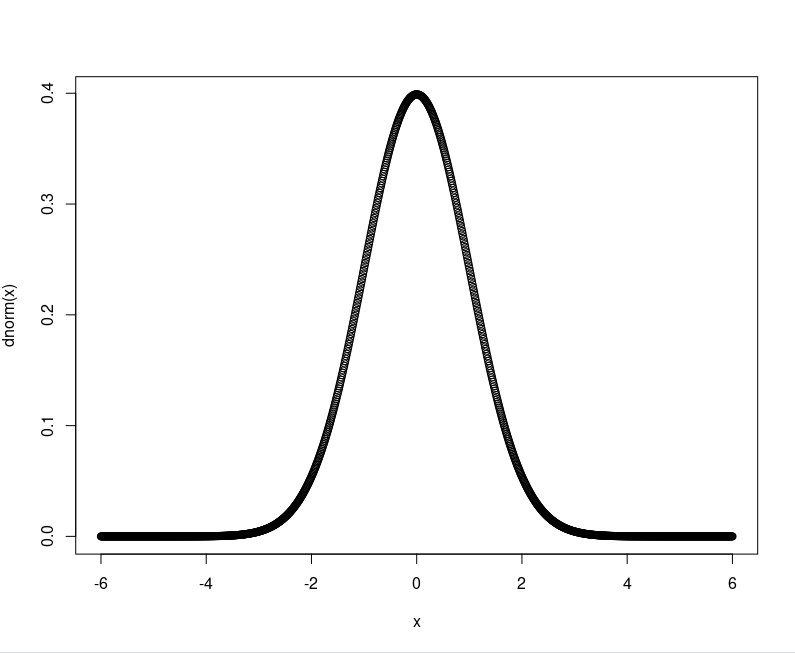
\includegraphics[width=3.35cm]{364a} }}
	\qquad
	\subfloat[]{{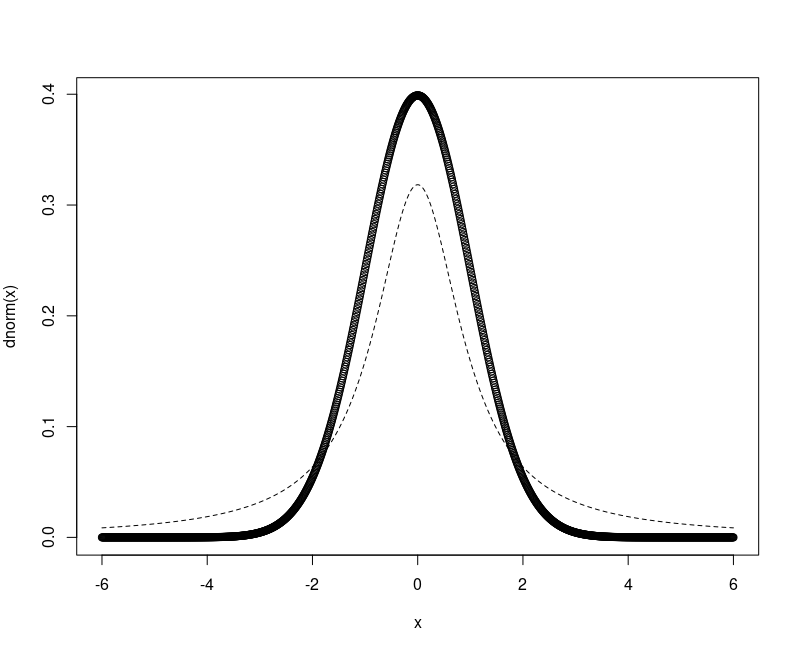
\includegraphics[width=3.35cm]{364b} }}
	\qquad
	\subfloat[]{{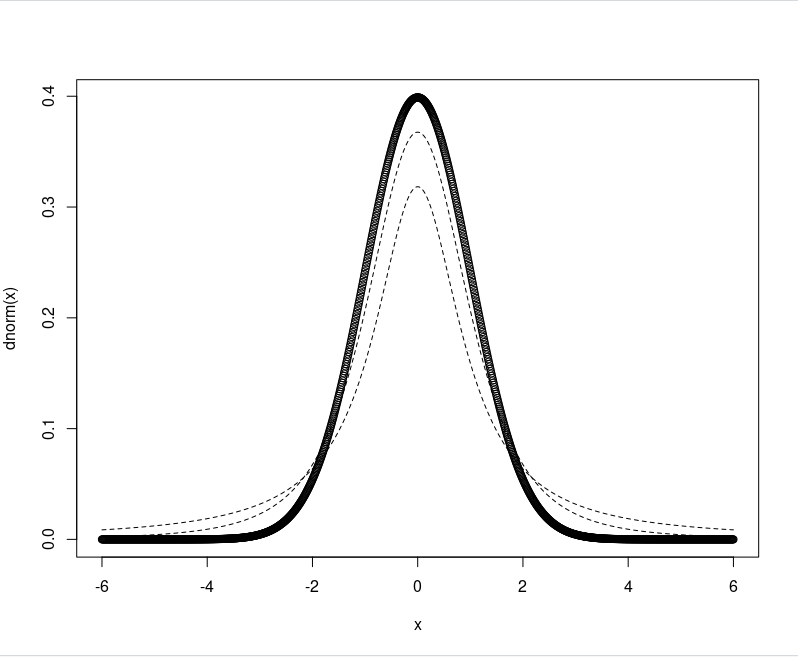
\includegraphics[width=3.35cm]{364c} }}\\
	\subfloat[]{{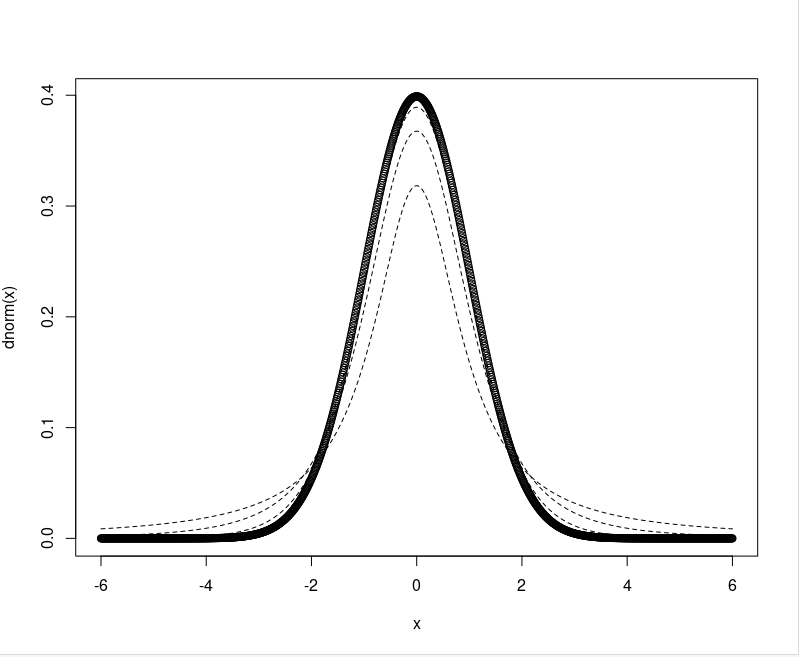
\includegraphics[width=4cm]{364d} }}
	\quad
	\subfloat[]{{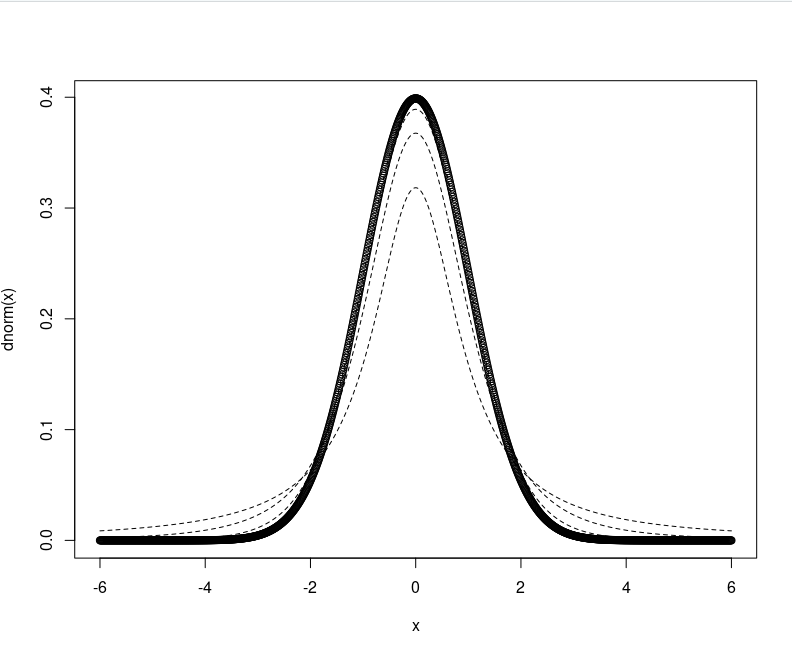
\includegraphics[width=4cm]{364e} }}
\end{figure}




\newpage
\noindent\textbf{3.6.5}
\begin{enumerate}[(a)] 
	\item $P(\abs{X} \geq 2) = 2\times[1 - P(X \leq 2)] = \textbf{0.046}$.
	\begin{lstlisting}
	> 2*(1 - pnorm(2))
	[1] 0.04550026
	\end{lstlisting}
	
	\item $P(\abs{X} \geq 2) = 2\times[1 - P(X \leq 2)] = \textbf{0.295}$.
	\begin{lstlisting}
	> 2*(1 - pt(2,1))
	[1] 0.2951672
	\end{lstlisting}
	
	\item $P(\abs{X} \geq 2) = 2\times[1 - P(X \leq 2)] = \textbf{0.139}$.
	\begin{lstlisting}
	> 2*(1 - pt(2,3))
	[1] 0.139326
	\end{lstlisting}
	
	\item $P(\abs{X} \geq 2) = 2\times[1 - P(X \leq 2)] = \textbf{0.073}$.
	\begin{lstlisting}
	> 2*(1 - pt(2,10))
	[1] 0.07338803
	\end{lstlisting}
	
	\item $P(\abs{X} \geq 2) = 2\times[1 - P(X \leq 2)] = \textbf{0.055}$.
	\begin{lstlisting}
	> 2*(1 - pt(2,30))
	[1] 0.05462504
	\end{lstlisting}
\end{enumerate}






\newpage
\noindent\textbf{3.6.11:} Let $T = W/\sqrt{V/r}$, where the independent variables $W \sim \mathcal{N}(0,1)$ and $V \sim \chi^2(r)$. Show that $T^2\sim F(r_1 = 1, r_2 = r)$. \textit{Hint}: What is the distribution of the numerator of $T^2$?\\

\noindent \textit{Solution:} Let the independent random variables $U,V$ be given, with $W\sim \N(0,1)$ and $U\sim \chi^2(r)$. The random variable $T^2$, where $T = W / \sqrt{V/r}$ is given by
\begin{align}
T^2 = \lp \f{W}{\sqrt{V/r}} \rp^2 = \f{W^2}{V/r}.
\end{align}
Because $W \sim \N(0,1)$, we have that $W^2 \sim \chi^2(1)$ (by theorem). Now, $T^2$ has the form 
\begin{align}
T^2 = \f{W^2}{V/r} = \f{W^2/1}{V/r}
\end{align}
where $1$ is the df of $\chi^2(1)$ which $W$ follows, and $r$ is the df of $\chi^2(r)$ which $U$ follows. Thus, $T^2 \sim F(1,r)$, by the definition of the $F$-distribution. \qed






\newpage

\noindent\textbf{3.6.15:} Let $X_1$, $X_2$ be iid with common distribution having the pdf 
\begin{align}
f(x) = \begin{cases}
e^{-x}, \quad 0< x < \infty\\
0, \quad \text{else}
\end{cases}
\end{align}
Show that $Z = X_1/X_2$ has an $F$-distribution.\\

\noindent \textit{Solution:}  It suffices to show that $Z$ can be written as a ratio of two $\chi^2$-distributed independent random variables. To this end, we can consider the mgf $M_X(t)$ of $X_1$, which is also identically that of $X_2$ since $X_1, X_2$ are iid:
\begin{align}
M_X(t) = E[e^{tx}] = \int^\infty_0 e^{tx}e^{-x} \,dx = (1-t)^{-1}.
\end{align}
However, this does not quite match the mgf for a $\chi^2(2)$. To circumvent this problem, we rewrite
\begin{align}
Z = \f{X_1}{X_2} =\f{2X_1/2}{2X_2/2}  = \f{(X_1+X_1)/2}{(X_2+X_2)/2},
\end{align}
as we expect $r=2$. Let $Y_1 = X_1 + X_1$. Then we have trivially $Y_1 =2X_1$, and so $\abs{J} = 1/2$. With this, $Y_1$ has the pdf 
\begin{align}
\tilde{f}_Y(y) = \abs{J}f(x) = \f{1}{2}f(x) = \begin{cases}
\f{1}{2}e^{-y/2}, \quad 0 < y < \infty\\
0, \quad \Else
\end{cases}. 
\end{align}
From here, we find the mgf of $Y_1$ to be 
\begin{align}
M_{Y_1}(t) = E[e^{ty}] = \f{1}{2}\int^\infty_{0}e^{ty}e^{-y/2}\,dy = (1-2t)^{-1} = (1-2t)^{-2/2}, t < \f{1}{2}.
\end{align}
By symmetry, $M_{Y_2}(t)$ is identically $M_{Y_1}(t)$, and both are the mgf for $\chi^2(r=2)$. Because each mgf uniquely determines a pdf, $Y_1, Y_2 \sim \chi^2(r=2)$ identically and independently (for each depends exclusively on $X_1$, $X_2$, respectively). Therefore, 
\begin{align}
Z = \f{(X_1+X_1)/2}{(X_2+X_2)/2} = \f{Y_1/2}{Y_2/2}
\end{align}
follows the $F$-distribution with degrees of freedom $r_1 = r_2 = 2$, by definition. \qed






\newpage
\noindent\textbf{3.6.16:} Let $X_1, X_2, X_3$ be independent r.v. with $X_i \sim \chi^2(r_i)$. 
\begin{enumerate}[(a)]
	\item Show that $Y_1 = X_1/X_2$ and $Y_2 = X_1 + X_2$ are independent and that $Y_2 \sim \chi^2(r_1 + r_2)$. 
	
	\item Deduce that 
	\begin{align}
	\f{X_1/r_1}{X_2/r_2} \text{ and } \f{X_3/r_3}{(X_1 + X_2)/(r_1 + r_2)}
	\end{align}
	are independent $F$-variables. 
\end{enumerate}

\noindent \textit{Solution:}  

\begin{enumerate}[(a)]
	\item We consider the transformation
	\begin{align}
	y_1 &= u(x_1,x_2) = \f{x_1}{x_2}\\
	y_2 &= v(x_1,x_2) = x_1 + x_2.
	\end{align}
	whose inverse is 
	\begin{align}
	x_1 = \bar{u}(y_1, y_2) = \f{y_1y_2}{1+y_1}\nn\\
	x_2 = \bar{v}(y_1, y_2) = \f{y_2}{1+y_1}.
	\end{align}
	The absolute value of the Jacobian is 
	\begin{align}
	\abs{J} = \abs{\det\begin{pmatrix}
		\p_{y_1}\bar{u} & \p_{y_2}\bar{u}\\
		\p_{y_1}\bar{v} & \p_{y_2}\bar{v}\\
		\end{pmatrix}} = \f{y_2}{(1+y_1)^2},
	\end{align}
	which maps one-to-one from the space of $X_1,X_2$ $\R^+\times \R^+$ onto the space of $Y_1, Y_2$ $\R^+\times \R^+$. Since $X_1, X_2$ are independent, we consider the joint pdf of $X_1, X_2$:
	\begin{align}
	h(x_1, x_2) = \begin{cases}
	\f{x_1^{r_1/2-1}x_2^{r_2/2-1}}{\Gamma(r_1/2)\Gamma(r_2/2)2^{(r_1+r_2)/2}}e^{-(x_1+x_2)/2}, \quad 0 < x_1,x_2 < \infty\\
	0, \quad \text{else}
	\end{cases}
	\end{align}
	from which we can deduce the joint pdf for $Y_1, Y_2$:
	\begin{align}
	\tilde{h}(y_1,y_2) &= \abs{J}h\lp \f{y_1y_2}{1+y_1}, \f{y_2}{1+y_1} \rp\nn\\
	&= \begin{cases}
	\f{y_2(y_1y_2)^{r_1/2-1}y_2^{r_2/2-1} (1+y_1)^{-r_1/2-r_2/2 + \cancel{ 2}}}{\cancel{(1+y_1)^2}\Gamma(r_1/2)\Gamma(r_2/2)2^{(r_1+r_2)/2}}e^{-y_2/2}, \,\, 0 < y_1,y_2 < \infty\\
	0, \quad \text{else}
	\end{cases}\nn\\
	&= \begin{cases}
	\f{y_2^{r_1/2+r_2/2-1}y_1^{r_1/2-1}(1+y_1)^{-r_1/2-r_2/2}}{\Gamma(r_1/2)\Gamma(r_2/2)2^{(r_1+r_2)/2}}e^{-y_2/2}, \,\, 0 < y_1,y_2 < \infty\\
	0, \quad \text{else}
	\end{cases}
	\end{align}
	Without further computation we see that $\tilde{h}(y_1,y_2)$ can be written as a product of two nonnegative functions of $y_1$ and $y_2$. In view of Theorem 2.4.1, $Y_1$ and $Y_2$ are independent. \qed \\
	
	Next, we wish to show $Y_2 \sim \chi^2(X_1, X_2)$, to which end we find the marginal pdf $g_2(y_2)$ of $Y_2$:
	\begin{align}
	g_2(y_2) &= \int^\infty_0 \tilde{h}(y_1,y_2)\,dy_1\nn\\
	&= \mathfrak{C}\int^\infty_0 {y_1^{r_1/2-1}(1+y_1)^{-r_1/2-r_2/2}}\,dy_1\nn\\
	&= \mathfrak{C}\f{\Gamma(r_1/2)\Gamma(r_2/2)}{\Gamma[(r_1+r_2)/2]}
	\end{align}
	where $\mathfrak{C}$ contains all the $y_1$-independent elements. From here, via simple back-substitution we obtain the marginal pdf for  $Y_2$:
	\begin{align}
	g_2(y_2) = \begin{cases}
	\f{y_2^{(r_1+r_2)/2 - 1 }}{\Gamma[(r_1+r_2)/2]2^{(r_1+r_2)/2}}e^{-y_2/2}, \quad 0 < y_2 < \infty\\
	0, \quad \Else
	\end{cases},
	\end{align}
	i.e., $Y_2 \sim \chi^2(r_1 + r_2)$. \qed\\
	
	\textbf{Mathematica code:}
	\begin{lstlisting}
	In[20]:= Integrate[
	x^(r1/2 - 1) (1 + x)^(-r1/2 - r2/2), {x, 0, Infinity}]
	
	Out[20]= ConditionalExpression[(Gamma[r1/2] Gamma[r2/2])/
	Gamma[(r1 + r2)/2], Re[r2] > 0 && Re[r1] > 0]
	\end{lstlisting}
	
	
	
	
	
	\item By definition, because $X_1, X_2$ are independent random variables with $X_i \sim \chi^2(r_i)$, 
	\begin{align}
	\Omega = \f{X_1/r_1}{X_2/r_2} \sim F(r_1, r_2).
	\end{align}
	Also, because $X_3 \sim \chi^2(r_3)$ and $(X_1 + X_2) \sim \chi^2(r_1 + r_2)$ (from (a)), we have
	\begin{align}
	\Lambda = \f{X_3/r_3}{(X_1 + X_2)/(r_1 + r_2)} \sim F(r_3, r_1 + r_2)
	\end{align}
	as well. Furthermore, because 
	\begin{align}
	&\Omega = \f{X_1/r_1}{X_2/r_2} = \f{r_2}{r_1}Y_1\\
	&\Lambda = \f{r_1+r_2}{r_3}\f{X_3}{Y_2}
	\end{align}
	and because $X_1, X_2, X_3$ are independent, we have that $Y_1, Y_2, X_3$ are independent. Therefore, it is necessary that $\Omega \sim F(r_1, r_2)$ and $\Lambda \sim F(r_3, r_1 + r_2)$ are independent as well. \qed
	
\end{enumerate}








\newpage




\textbf{4.1.1} Twenty motors were put on test under a high-temperature setting. The
lifetimes in hours of the motors under these conditions are given below. Also, the
data are in the file \textbf{lifetimemotor.rda} at the site listed in the Preface. Suppose
we assume that the lifetime of a motor under these conditions, $X$, has a $\Gamma(1, \theta)$
distribution.\\

\begin{tabular}{c c c c c c c c c c }
	1 &4& 5& 21& 22& 28& 40& 42& 51& 53\\
	58 &67& 95& 124& 124& 160& 202& 260& 303& 363
\end{tabular}


\begin{enumerate}[(a)]
	\item Obtain a histogram of the data and overlay it with a density estimate, using
	the code \textbf{hist(x,pr=T); lines(density(x))} where the R vector\textbf{x} contains
	the data. Based on this plot, do you think that the $\Gamma(1, \theta)$ model is credible?
	
	\item Assuming a $\Gamma(1, \theta)$ model, obtain the maximum likelihood estimate $\hat{\theta}$ of $\theta$ and locate it on your histogram. Next overlay the pdf of a $\Gamma(1, \hat{\theta})$ distribution on the histogram. Use the R function \textbf{dgamma(x,shape=1,scale=$\hat{\theta}$)} to evaluate the pdf.
	
	\item Obtain the sample median of the data, which is an estimate of the median
	lifetime of a motor. What parameter is it estimating (i.e., determine the
	median of $X$)?
	
	\item Based on the mle, what is another estimate of the median of $X$?
\end{enumerate}


\noindent \textit{Solution:}  
\begin{enumerate}[(a)]
	\item For some reason R does not recognize the dataset as of numeric type. Because the dataset is small enough, I recoded and fed it by hand to the data vector $y$:
	\begin{lstlisting}
	> lines(density(y))
	> y <- c(1,4,5,21,22,28,40,42,51,53,58,67,
	95,124,124,160,202,260,303,363)
	> hist(y,pr=T)
	> lines(density(y))
	\end{lstlisting}
	\begin{figure}[!htb]
		\centering
		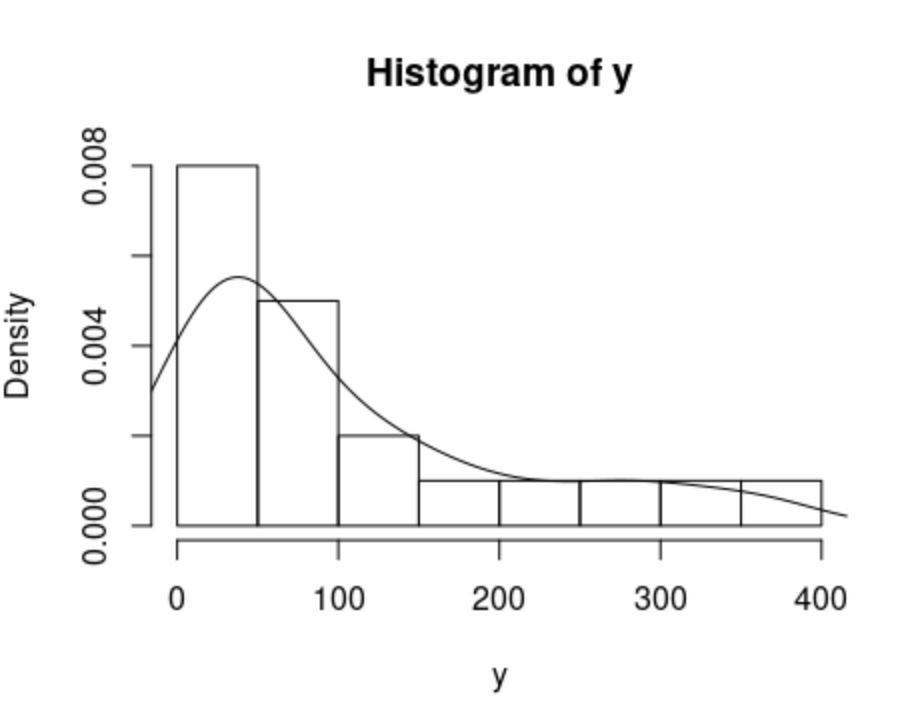
\includegraphics[scale=0.3]{411a}
	\end{figure}
	The $\Gamma(1,\theta)$, or $\text{Exp}(\theta)$, model seems to be \textbf{credible} as far as the histogram is concerned. However, the overlaying density does not look like a $\Gamma(1,\theta)$. \qed
	
	
	
	\item Assuming the $\Gamma(1,\theta)$ model, then the pdf on the support $\R^+$ is given by
	\begin{align}
	f(y) = \f{1}{\theta}e^{-y/\theta},
	\end{align}
	from which we obtain the logarithm of the likelihood function:
	\begin{align}
	l(\theta) = \log\lp \prod^n_{i=1} \f{1}{\theta}e^{-y_i/\theta} \rp = -n\log\theta - \f{1}{\theta}\sum^n_{i=1}y_i.
	\end{align}
	The first partial derivative wrt $\theta$ is then
	\begin{align}
	\p_\theta l(\theta) = -\f{n}{\theta} + \f{1}{\theta^2}\sum^n_{i=1}y_i.
	\end{align}
	Setting $\p_\theta l(\theta) = 0$, we get (by inspection) that $l(\theta)$ is extremized iff $\theta = (1/n)\sum^n_{i=1}y_i = \bar{y}$. We also have that $\p_{\theta\theta} < 0\, \forall \theta \in \R^+$, which means $l(\theta)$ is maximized globally at $\bar{y}$. From here, the statistic 
	\begin{align}
	\hat{\theta} = \bar{Y} = \mathbf{101.15}
	\end{align} 
	is the mle of $\theta$. (Also note that because $E[Y] = \theta \implies E[\bar{Y}] = \theta$, $\hat{\theta}$ is an unbiased estimator of $\theta$.)
	\begin{lstlisting}
	> mean(y)
	[1] 101.15
	> abline(v = mean(y), lwd=3, lty=2)
	> z=dgamma(y, shape=1, scale=mean(y))
	> lines(z~y,lty=2)
	\end{lstlisting}
	\begin{figure}[!htb]
		\centering
		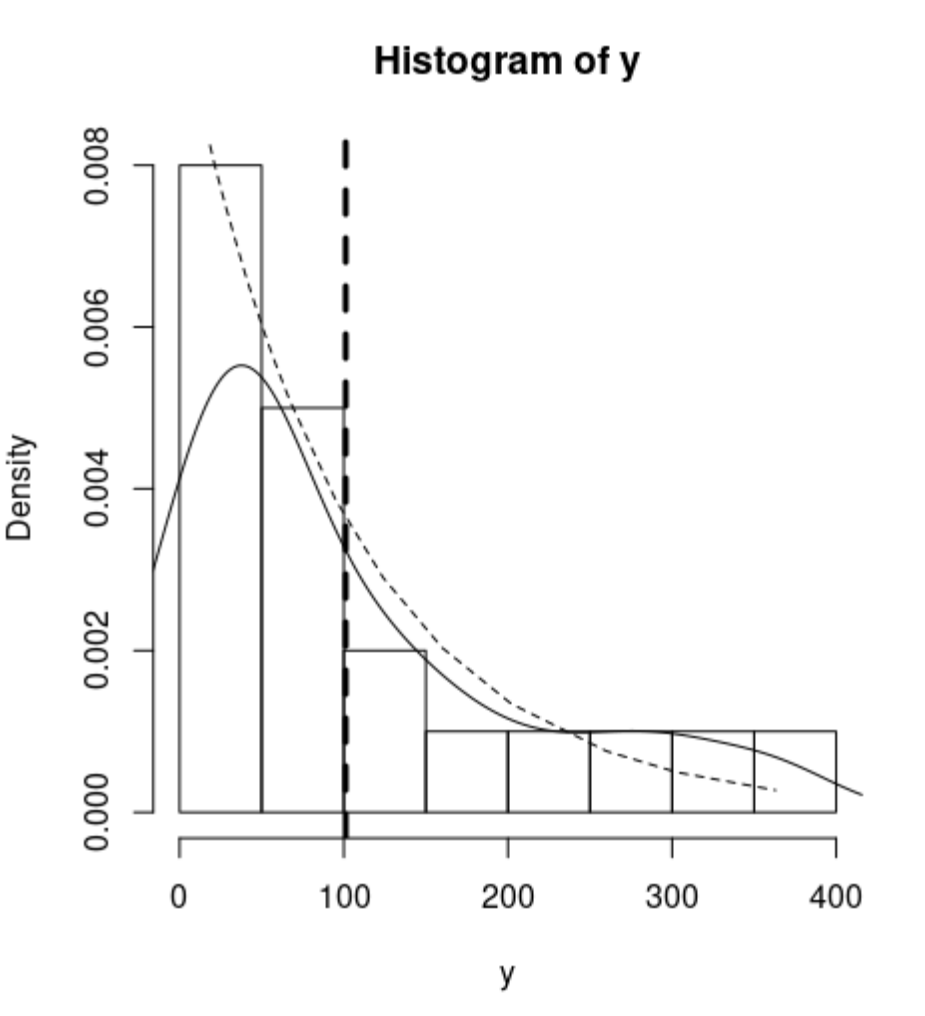
\includegraphics[scale=0.3]{411b}
	\end{figure}
	
	
	
	
	\item The sample median of the data is \textbf{55.5}
	\begin{lstlisting}
	> median(y)
	[1] 55.5
	\end{lstlisting}
	The median of $Y \sim \Gamma(1,\theta) \equiv \text{Exp}(\theta)$ is the value of $y'$ at which 
	\begin{align}
	0.5 = \int^{y'}_{0}\f{1}{\theta}e^{-y/\theta}\,dy = 1 - e^{-y'/\theta} \implies y' = \theta \ln 2,
	\end{align} 
	which means that the median of $Y \sim \Gamma(1,\theta) \equiv \text{Exp}(1,\theta)$ is the half-life, $\theta \ln 2$. Since the sample median is just $\theta$ multiplied by $\ln 2$, the sample median also estimates the parameter $\theta$. 
	
	
	
	\item From part (a), we know that $\hat{\theta} = \bar{Y}$, the sample mean, is the mle of $\theta$, the population mean. From part (c), we have shown that the median of $Y \sim \Gamma(1,\theta)$ is simply $\theta \ln 2$. By simple inspection we see that $\hat{\theta}\ln 2 = \hat{Y} \ln 2$ is the (\textit{unbiased}) mle of $\theta \ln 2$, the median of $Y$. \qed 
	
	
	
\end{enumerate}








\newpage

\noindent \textbf{4.1.3} Suppose the number of customers $X$ that enter a store between the hours
9:00 a.m. and 10:00 a.m. follows a Poisson distribution with parameter $\theta$. Suppose
a random sample of the number of customers that enter the store between 9:00 a.m.
and 10:00 a.m. for 10 days results in the values\\

\begin{tabular}{c c c c c c c c c c}
	9& 7& 9 &15& 10& 13& 11& 7 &2& 12
\end{tabular}


\begin{enumerate}
	\item Determine the maximum likelihood estimate of $\theta$. Show that it is an unbiased
	estimator.
	
	\item Based on these data, obtain the realization of your estimator in part (a).
	Explain the meaning of this estimate in terms of the number of customers.
	
\end{enumerate}


\noindent \textit{Solution:} 
\begin{enumerate}
	\item Let $X \sim \text{Poi}(\theta)$ be given, then the pmf of $X$ is given by
	\begin{align}
	p(x) = \begin{cases}
	\f{\theta^x e^{-\theta}}{x!}, \quad x\in \mathbb{N}\\ 
	0, \quad \Else
	\end{cases}.
	\end{align}
	Assuming the $X_i$'s $\sim \text{Poi}(\theta)$ are iid, where $i=1,\dots,n$, then the logarithm of the likelihood function is 
	\begin{align}
	l(\theta) &= \log \lp \prod^n_{i=1} \f{\theta^{x_i} e^{-\theta}}{x_i!} \rp\nn\\
	&= \log \lp e^{-n\theta}\theta^{\sum_{i=1}^n x_i}  \prod^n_{i=1}\f{1}{x_i!} \rp\nn\\
	&= -n\theta + \lp \sum^n_{i=1}x_i\rp\log \theta - \sum^n_{i=1}\log x_i!. 
	\end{align}
	Setting $\p_\theta l(\theta) = 0$, we solve for $\theta$:
	\begin{align}
	\p_\theta l(\theta) = -n +  \f{1}{\theta}\sum^n_{i=1}x_i = 0 \iff \theta = \f{1}{n}\sum^n_{i=1} x_i = \bar{x}
	\end{align}
	By inspection, $\p_{\theta\theta}l(\theta) < 0 \forall \theta \in \mathbb{R}^+$, and so the statistic
	\begin{align}
	\hat{\theta} = \bar{Y}
	\end{align}
	is the mle of $\theta$. Further, it is an unbiased estimator of $\theta$ simply because
	\begin{align}
	E[Y] =  \theta \implies E[\bar{Y}] = \theta.
	\end{align}
	\qed
	
	
	\item Part (a) says the sample means is the mle of $\theta$. The means of the given sample is \textbf{9.5}.
	\begin{lstlisting}
	> mean(c(9 ,7, 9, 15, 10, 13, 11, 7, 2, 12))
	[1] 9.5
	\end{lstlisting}
	This says that on average, 9.5, or about 9-10 customers enter the store between the hours 9:00 a.m. and 10:00 a.m.. \qed
	
	
	
\end{enumerate}












\newpage
\noindent \textbf{4.1.8} Recall that for the parameter $\eta = g(\theta)$, the mle of $\eta$ is $g(\hat{\theta})$, where $\hat{\theta}$ is the mle of $\theta$. Assuming that the data in Example 4.1.6 were drawn from a Poisson distribution with mean $\lambda$, obtain the mle of $\lambda$ and then use it to obtain the mle of the pmf. Compare the mle of the pmf to the nonparametric estimate. Note: For the domain value 6, obtain the mle of $P(X \geq 6)$.\\

\noindent \textit{Solution:} Based on the previous problem, the mle of $\lambda$ is the sample means, which has the value \textbf{2.13}.
\begin{lstlisting}
> mean(c(2,1,1,1,1,5,1,1,3,0,2,1,1,3,4,2,1,2,2,6,5,2,3,2,4,1,3,1,3,0))
[1] 2.133333
\end{lstlisting}
Because the sample means $\bar{x}$ is the mle of $\lambda$, and the pmf is given by
\begin{align}
p(x) = \begin{cases}
\f{\lambda^x e^{-\lambda}}{x!}, \quad x \in \mathbb{N}\\ 
0, \quad \Else
\end{cases},
\end{align}
the mle of the pmf is given by
\begin{align}
\tilde{p}(x) = \begin{cases}
\f{\bar{x}^x e^{-\bar{x}}}{x!}, \quad x \in \mathbb{N}\\ 
0, \quad \Else
\end{cases}.
\end{align}
Next, we compare the mle of the pmf to the nonparametric estimate:\\

\begin{tabular}{ c c c c c c c c}
	j & 0 &1& 2& 3& 4& 5& $\geq$ 6 \\
	$\hat{p}(j)$& 0.067 & 0.367 & 0.233 & 0.167 & 0.067 & 0.067 & 0.033\\
	$\tilde{p}(j)$ & 0.118 & 0.253 & 0.270  & 0.192  & 0.102 & 0.044  &  0.022
\end{tabular}\\


\textbf{Mathematica code for $P(j \geq 6)$ for $\tilde{p}(j)$:}
\begin{lstlisting}
P[x_] := (2.1333333)^x*E^(-2.1333333)/x!

N[Sum[P[y], {y, 6, Infinity}]]

0.0218705
\end{lstlisting}






\newpage

\section{Problem Set 2}




\noindent \textbf{4.2.2.} Consider the data on the lifetimes of motors given in Exercise 4.1.1. Obtain
a large sample 95\% confidence interval for the mean lifetime of a motor.\\

\noindent \textit{Solution:} Large sample $95\%$ CI's have the form
\begin{align}
(\bar{x}- z_{\alpha/2}\f{S}{\sqrt{n}} , \bar{x}+ z_{\alpha/2}\f{S}{\sqrt{n}})
\end{align}
Here, $\bar{x} = 101.15, n= 20, s = 105.4091, z_{\alpha/2} = 1.96$. So, the desired CI is
\begin{align}
(101.15- 1.96\f{105.4091}{\sqrt{20}} , 101.15+ 1.96\f{105.4091}{\sqrt{20}}) = \boxed{(54.95, 147.35)}
\end{align}\qed





\newpage
\noindent\textbf{4.2.6.} $\overline{X}$ is the sample mean of a sample of size $n$ from $\N(\mu,9)$. Find $n$ such that 
\begin{align}
P(\bar{X}-1\leq \mu \leq \bar{X}+1) = 0.90
\end{align}

\noindent \textit{Solution:}  $\sigma^2 = 9 \implies \sigma = 3$. We have
\begin{align}
0.90 &= P( \bar{X} - 1\leq \mu \leq \bar{X} + 1 )\nn\\
&= P\lp \mu - 1  \leq \bar{X} \leq \mu+1  \rp \nn\\
&= P\lp -1 \leq \bar{X} - \mu \leq 1  \rp\nn\\
&= P\lp \f{-1}{3/\sqrt{n}} \leq \f{\bar{X}-\mu}{3/\sqrt{n}} \leq \f{1}{3/\sqrt{n}} \rp.
\end{align} 
In other words,
\begin{align}
z_{0.05} = \f{1}{3/\sqrt{n}} = \f{\sqrt{n}}{3} = 1.644854 \implies n = 24.35 \approx\boxed{25}.
\end{align}\qed



\newpage
\noindent\textbf{4.2.18.} $X_i$'s $\sim \N(\mu,\sigma^2)$, with $\mu,\sigma^2$ unknown. A confidence interval for $\sigma^2$ can be found as follows.
We know that $(n-1)S^2/\sigma^2$ is a random variable with a $\chi^2(n−1)$ distribution. Thus
we can find constants $a$ and $b$ so that $P((n - 1)S^2/σ\sigma^2 < b)=0.975$ and $P(a <
(n - 1)S^2/\sigma^2 < b)=0.95$. In R, $b = qchisq(0.975,n-1)$, while $a = qchisq(0.025,n-1).$


\begin{enumerate}[(a)]
	\item Show that this second probability statement can be written as
	\begin{align}
	P((n - 1)S^2/b < \sigma^2 < (n - 1)S^2/a)=0.95.
	\end{align}
	\item If $n = 9$ and $S^2 = 7.93$, find a 95\% confidence interval for $\sigma^2$.
	\item If $\mu$ is known, how would you modify the preceding procedure for finding a
	confidence interval for $\sigma^2$?
\end{enumerate}


\noindent \textit{Solution:}

\begin{enumerate}[(a)]
	\item We simply re-arrange things in the probability statement:
	\begin{align}
	0.95 &= P(a < (n-1)S^2/\sigma^2 < b) \nn\\
	&= P(\sigma^2 < (n-1)S^2/a \land \sigma^2 > (n-1)S^2/b)\nn\\
	&= P((n-1)S^2/b < \sigma^2 < (n-1)S^2/a).
	\end{align}
	
	\item When $n=9, s^2 = 7.93$, we have $a=2.179731$ and $b=17.53455$. Then the $95\%$ CI for $\sigma^2$ is
	\begin{align}
	\lp \f{(n-1)S^2}{b} , \f{(n-1)S^2}{a} \rp  = \lp \f{8\times 7.93}{17.53455}, \f{8\times 7.93}{2.179731} \rp = \boxed{\lp 3.618, 29.10451 \rp}
	\end{align}
	
	\item If $\mu$ is known, the unbiased estimator for the population standard deviation becomes proportional to $1/\sqrt{n}$, not $1/\sqrt{n-1}$. Because of this, we modify some numerics in our procedure from $n-1$ to $n$. From here, we make the following changes
	\begin{align}
	&(n-1)S^2/\sigma^2 \sim \chi^2(n-1) \to nS^2/\sigma^2 \sim \chi^2(n) \nn\\
	&P(nS^2/\sigma^2 < b) = 0.975\nn\\
	&P(a<nS^2/\sigma^2<b) = 0.95. 
	\end{align}
	The new CI will look like $(nS^2/b < \sigma^2 < nS^2/a)$.
\end{enumerate}\qed




 
\newpage
\noindent\textbf{4.2.21.} Let two independent random samples, each of size 10, from two normal
distributions $\N(\mu_1, \sigma^2)$ and $\N(\mu_2, \sigma^2)$ yield $\bar{x} = 4.8, s^2_1 = 8.64, \bar{y} = 5.6, s^2_2 = 7.88$. Find a 95\% confidence interval for $\mu_1 - \mu_2$.\\

\noindent \textit{Solution:} The 95\% CI for difference in means i this case looks like
\begin{align}
\lp (\bar{x} - \bar{y}) - t_{\al/2,n_1+n_2-2}s_p\sqrt{\f{1}{n_1}+\f{1}{n_2}} , (\bar{x} - \bar{y}) + t_{\al/2,n_1+n_2-2}s_p\sqrt{\f{1}{n_1}+\f{1}{n_2}}   \rp.
\end{align}
The pooled variance is
\begin{align}
s_p^2 = \f{(n_1-1)s_1^2 + (n_2-1)s_2^2}{n_1+n_2-2} = \f{9\times 8.65 + 9\times 7.88}{18} = 8.26.
\end{align}
Plugging in numbers we find the CI, with $t_{0.025,18} =2.100922$:
\begin{align}
\lp (4.8-5.6) - 2.100922\sqrt{8.26}\sqrt{\f{1}{10}+\f{1}{10}} , (4.8-5.6) + 2.100922\sqrt{8.26}\sqrt{\f{1}{10}+\f{1}{10}}   \rp\nn\\
 = \boxed{\lp -3.500, 1.900 \rp}
\end{align}\qed











\newpage
\noindent\textbf{4.2.22.} Let two independent random variables, $Y_1$ and $Y_2$, with binomial distributions that have parameters $n_1 = n_2 = 100$, $p_1$, and $p_2$, respectively, be observed
to be equal to $y_1 = 50$ and $y_2 = 40$. Determine an approximate 90\% confidence
interval for $p_1 - p_2$.\\



\noindent \textit{Solution:} The $90\%$ CI for the difference in proportions looks like
\begin{align}
\lp (\hat{p_1} - \hat{p_2}) - z_{\alpha/2}\sqrt{\f{\hat{p_1}(1-\hat{p_1})}{n_1} + \f{\hat{p_2}(1-\hat{p_2})}{n_2}} , \right.\nn\\ \left. (\hat{p_1} - \hat{p_2}) + z_{\alpha/2}\sqrt{\f{\hat{p_1}(1-\hat{p_1})}{n_1} + \f{\hat{p_2}(1-\hat{p_2})}{n_2}} \rp
\end{align}
where $\alpha_{0.05} = 1.644854$. Plugging in numbers, we find
\begin{align}
&\lp 0.5-0.4 - 1.644854\sqrt{ \f{(0.5)(0.5)}{100} + \f{(0.4)(0.6)}{100} },\right.\nn\\ &\quad \left. 0.5-0.4 + 1.644854\sqrt{ \f{(0.5)(0.5)}{100} + \f{(0.4)(0.6)}{100} }  \rp\nn\\
 = &\boxed{ (-0.01513978,0.2151398) }
\end{align}\qed



\newpage
\noindent\textbf{4.2.27.} Let $X_1, X_2,\dots,X_n$ and $Y_1, Y_2,\dots,Y_m$ be two independent random samples
from the respective normal distributions $\N(\mu_1, \sigma^2_1)$ and $\N(\mu_2, \sigma^2_2)$, where the four
parameters are unknown. To construct a confidence interval for the ratio, $\sigma^2_1/\sigma^2_2$, of
the variances, form the quotient of the two independent χ2 variables, each divided
by its degrees of freedom, namely,
\begin{align}
F = \f{\f{(m-1)S_2^2}{\sigma^2_2}/(m-1)}{\f{(n-1)S_1^2}{\sigma^2_1}/(n-1)} = \f{S_2^2/\sigma_2^2}{S_1^2/\sigma_1^2}
\end{align}
where $S_1^2, S_2^2$ are respectively sample variances. 

\begin{enumerate}[(a)]
	\item What kind of distribution does $F$ have?
	\item Rewrite the second probability statement as
	\begin{align}
	P \lb a\f{S_1^2}{S_2^2} < \f{\sigma_1^2}{\sigma_2^2} < b \f{S_1^2}{S^2_2} \rb = 0.95.
	\end{align}
	The observed values, $s^2_1$ and $s_2^2$, can be inserted in these inequalities to provide
	a 95\% confidence interval for $\sigma^2_1/σ^2_2$. 
\end{enumerate}


\noindent \textit{Solution:} 
\begin{enumerate}[(a)]
	\item $F\sim F(m-1,n-1)$, by definition. 
	\item We just rearrange the quantities in the probability statement:
	\begin{align}
	0.95 &= P(a<F<b) \nn\\
	&= P\lp a < \f{S_2^2/\sigma_2^2}{S_1^2/\sigma_1^2} < b  \rp\nn\\
	&= P\lp \f{\sigma_1^2}{\sigma_2^2} < b\f{S_1^2}{S_2^2} \land \f{\sigma_1^2}{\sigma_2^2} > a \f{S_1^2}{S_2^2}  \rp\nn\\
	&= P\lp   a \f{S_1^2}{S_2^2} <  \f{\sigma_1^2}{\sigma_2^2}  < b \f{S_1^2}{S_2^2} \rp.
	\end{align}
\end{enumerate}\qed
















\newpage
\noindent\textbf{4.5.1.} Show that the approximate power function given in expression (4.5.12) of
Example 4.5.3 is a strictly increasing function of $\mu$. Show then that the test discussed
in this example has approximate size $\alpha$ for testing
\begin{align}
H_0: \mu \leq \mu_0\quad \text{versus} \quad H_1: \mu > \mu_0.
\end{align}


\noindent \textit{Solution:} The approximate power function is given by
\begin{align}
\gamma(\mu) \approx \Phi \lp -z_\alpha - \f{\sqrt{n}(\mu_0 - \mu)}{\sigma} \rp
\end{align}
$\p_\mu \gamma(\mu)$ is necessarily positive $\forall \mu \in \mathbb{R}$ for $\gamma(\mu)$ to be strictly increasing. So we check:
\begin{align}
\p_\mu \gamma(\mu) &= \p_\mu \lb \Phi \lp -z_\alpha - \f{\sqrt{n}(\mu_0 - \mu)}{\sigma} \rp  \rb \nn\\
&= \Phi' \lp -z_\alpha - \f{\sqrt{n}(\mu_0 - \mu)}{\sigma} \rp \f{\sqrt{n}}{\sigma}.
\end{align}
We note that $\sqrt{n}/\sigma > 0$ and $\Phi'(\dots) > 0$ necessarily because $\Phi$ is a cdf (for the $\N(\mu,\sigma^2)$). With this, we have shown that $\gamma(\mu)$ is strictly increasing in $\mu$.\\

\noindent Under the hypotheses and the fact that $\gamma(\mu)$ is strictly increasing in $\mu$, $\al = \max_{\mu \leq \mu_0}$ is maximized whenever $\mu \leq \mu_0$ is maximized, i.e. $\mu = \mu_0$:
\begin{align}
\max_{\mu \leq \mu_0} \gamma(\mu) = \gamma(\mu_0) = \Phi(-z_\alpha) = \alpha.
\end{align}
So the test has approximate size $\alpha$. \qed







\newpage
\noindent\textbf{4.5.2.} For the Darwin data tabled in Example 4.5.5, verify that the Student t-test
statistic is 2.15. \\


\noindent \textit{Solution:} $\al = 0.05$. The sample mean and standard deviation for the differences are
\begin{align}
&\bar{x} = 2.62\\
&s_x = 4.71826.
\end{align}
The t-statistic is then
\begin{align}
t_{df=14}= \f{\bar{x}-0}{s_x} = \f{2.62}{4.71826/\sqrt{15}} \approx \boxed{2.150627}
\end{align}



\textbf{R code:}
\begin{lstlisting}
> mean(darwin$cross)-mean(darwin$self)
[1] 2.62

> sd(darwin$cross - darwin$self)
[1] 4.71826
\end{lstlisting}
\qed










\newpage
\noindent\textbf{4.5.5.} Let $X_1, X_2$ be a random sample of size $n = 2$ from the distribution having
pdf $f(x; \theta) = (1/\theta)e^{-x/\theta}, \theta <x< \infty$, zero elsewhere. We reject $H_0 : \theta = 2$ and
accept $H_1 : \theta = 1$ if the observed values of $X_1, X_2$, say $x_1, x_2$, are such that
\begin{align}
\f{f(x_1;2)f(x_2;2)}{f(x_1;1)f(x_2;1)} \leq \f{1}{2}
\end{align}
Here $\Omega = \{\theta : \theta = 1, 2\}$. Find the significance level of the test and the power of the
test when $H_0$ is false.\\



\noindent \textit{Solution:}  We reject $H_0$ whenever
\begin{align}
\f{1}{2} &\geq \f{f(x_1;2)f(x_2;2)}{f(x_1;1)f(x_2;1)}\nn\\
&=\f{(1/2)e^{-x_1/2}(1/2)e^{-x_2/2}}{e^{-x_1}e^{-x_2}} \nn\\
&= \f{1}{4}e^{x_1/2}e^{x_2/2}\nn\\
&= \f{1}{4}e^{(x_1+x_2)/2} \implies x_1+x_2 \leq 2\ln(2). 
\end{align}
The significance level of the test $\alpha$ is the probability of rejecting $H_0$ when it is true, i.e.
\begin{align}
\alpha = P(x_1+x_2 \leq 2\ln(2)\vert \theta = 2).
\end{align} 
Recall that the non-zero part of the pdf for $\Gamma(k,\theta)$ is given by
\begin{align}
f(x) &= \f{1}{\Gamma(k)\theta^k}x^{k-1}e^{-x/\theta}, \quad x\in \mathbb{R}^+\nn\\
&= \f{1}{\theta^1}e^{-x/\theta}, \quad k=1,
\end{align}
we have that $X_1,X_2 \sim \Gamma(k=1,\theta=2)$, iid, implies $X_1+X_2 \sim \Gamma(k= 2, \theta = 2)$. From here, it is ``easy'' to calculate $\alpha$:
\begin{align}
\alpha &= P(x_1+x_2 \leq 2\ln(2)\vert \theta = 2) = \int^{2\ln(2)}_0 \f{1}{\Gamma(2)\theta^2}\xi e^{-\xi/\theta}\,d\xi\nn\\
&= \int^{2\ln(2)}_0 \f{1}{4}\xi e^{-\xi/2}\,d\xi\nn\\
&= \f{1}{2}(1-\ln(2)) \approx \boxed{0.1534}
\end{align}

The power of the test is the probability of rejecting $H_0$ when $H_0$ is false. In this case, we make a similar calculation, only setting $\theta = 1$ (since $H_0$ false):
\begin{align}
P(x_1+x_2 \leq 2\ln(2)\vert \theta = 1) &= \int^{2\ln(2)}_0 \xi e^{-\xi}\,d\xi \nn\\
&= \f{3}{4} - \f{\ln(2)}{2} \approx \boxed{0.403426}
\end{align}\qed














\newpage
\noindent\textbf{4.5.12.} Let $X_1, X_2,\dots,X_8$ be a random sample of size $n = 8$ from a Poisson
distribution with mean $\mu$. Reject the simple null hypothesis $H_0 : \mu = 0.5$ and
accept $H_1 : \mu > 0.5$ if the observed $\sum^8_{i=1} x_i \geq 8.$
\begin{enumerate}[(a)]
	\item Show that the significance level is \texttt{1-ppois(7,8*.5).}
	\item Use R to determine $\gamma(0.75)$, $\gamma(1)$, and $\gamma(1.25)$.
	\item Modify the code in Exercise 4.5.9 to obtain a plot of the power function.
\end{enumerate}


\noindent \textit{Solution:} 
\begin{enumerate}[(a)]
	\item The significance level $\al$ is the probability of rejecting $H_0$ when $H_0$ is true. Under the null, $\mu = 0.5$, and the r.v.
	\begin{align}
	X_1 + \dots + X_8 \sim \text{Poi}(8\mu) \equiv \text{Poi}(8\times 0.5).
	\end{align}
	$\alpha$ is given by
	\begin{align}
	\alpha = \gamma(\mu)  &= P\lp \sum^8_{i=1} x_i \geq 8 \vert \mu = 0.5 \rp\nn\\
	&= 1 - P\lp \sum^8_{i=1}x_i < 7 \rp\nn\\
	&= \boxed{1 - \texttt{ppois(7,8*.5)}}\nn\\
	&= 0.05113362
	\end{align}
	
	\item 
	\begin{align}
	\gamma(0.75) = \boxed{0.2560202}\nn\\
	\gamma(1) = \boxed{0.5470392}\nn\\
	\gamma(1.25) = \boxed{0.7797794}
	\end{align}
	\textbf{R code:}
	\begin{lstlisting}
	> 1 - ppois(7,8*0.5)
	[1] 0.05113362
	
	> 1 - ppois(7,8*0.75)
	[1] 0.2560202
	
	> 1 - ppois(7,8*1)
	[1] 0.5470392
	
	> 1 - ppois(7,8*1.25)
	[1] 0.7797794
	\end{lstlisting}
	\item 	\textbf{R code:}
	\begin{lstlisting}
> theta=seq(.75,1.25,.25); gam=1-ppois(7,theta*8)
> plot(gam~theta,pch=" ",xlab=expression(theta),ylab=expression(gamma))
> lines(gam~theta)
	\end{lstlisting}
	We're interested in the range of $\theta \in [0.75, 1.25]$. I'm making the step size small to make the power function look smooth.\\
	
	
	
	\noindent Plot of $\gamma(\mu)$:
	\begin{figure}[!htb]
		\centering
		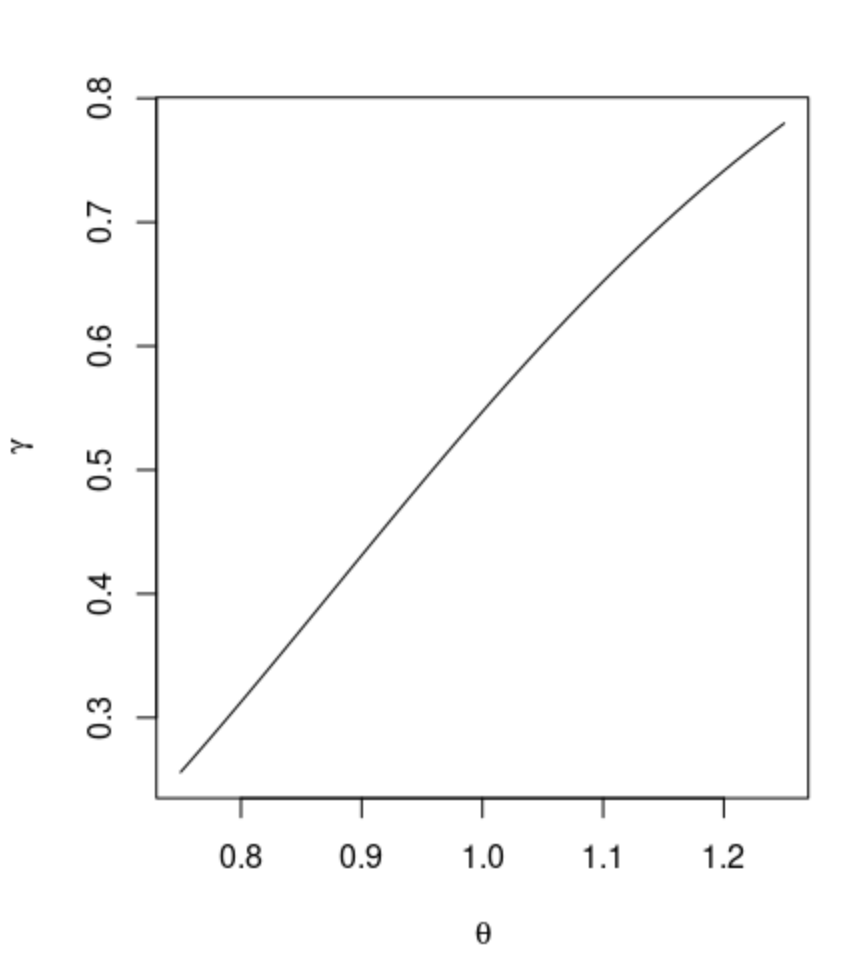
\includegraphics[scale=0.35]{power}
	\end{figure} 
	

\end{enumerate}
\qed












\newpage
\noindent \textbf{4.6.4.} (Note that it is fine to make a heuristic argument here. Just make sure that it is clear with
supporting graphs/figures (hand drawn is fine).) Consider the one-sided t-test for $H_0 : \mu = \mu_0$ versus $H_{A1} : \mu>\mu_0$ constructed in Example 4.5.4 and the two-sided t-test for t-test for $H_0 : \mu = \mu_0$ versus
$H_1 : \mu = \mu_0$ given in (4.6.9). Assume that both tests are of size $\alpha$. Show that for
$\mu>\mu_0$, the power function of the one-sided test is larger than the power function of the two-sided test.\\


\noindent \textit{Solution:} We want to show that for $\mu > \mu_0$, the power function of the one-sided test is larger than the power function of the two-sided test. To this end, let $\gamma_1(\mu)$ denote the power function of the one-sided test, and $\gamma_2(\mu)$ the two-sided test. This gives
\begin{align}
\gamma_2(\mu) = P\lp \abs{\text{test-statistic}} \geq t_{\alpha/2,n-1} \rp = P\lp {\text{test-statistic}} \geq t_{\alpha/2,n-1} \rp
\end{align}
(test statistic positive because $\mu > \mu_0$), while 
\begin{align}
\gamma_1(\mu) = P\lp \text{test-statistic} \geq t_{\alpha,n-1} \rp.
\end{align}
Since $t_{\alpha/2,n-1} > t_{\alpha,n-1} $ , we have that 
\begin{align}
\gamma_2(\mu) = P(\abs{\cdot} \geq t_{\alpha/2}) \leq P(\cdot \geq t_\al) = \gamma_1(\mu).
\end{align}
And so, for a given $\mu > \mu_0$, the power function of the one-sided test is larger than the power function of the two-sided test. \qed





















\newpage
\noindent \textbf{4.6.7.} Among the data collected for the World Health Organization air quality
monitoring project is a measure of suspended particles in $\mu$g/m$^3$. Let $X$ and $Y$ equal
the concentration of suspended particles in $\mu$g/m$^3$ in the city center (commercial
district) for Melbourne and Houston, respectively. Using $n = 13$ observations of $X$
and $m = 16$ observations of $Y$ , we test $H_0 : \mu_X = \mu_Y$ against $H_1 : \mu_X < \mu_Y$.

\begin{enumerate}[(a)]
	\item Define the test statistic and critical region, assuming that the unknown variances are equal. Let $\al = 0.05$.
	\item If $\bar{x} = 72.9$, $s_x = 25.6$, $\bar{y} = 81.7$, and $s_y = 28.3$, calculate the value of the
	test statistic and state your conclusion.
\end{enumerate}


\noindent \textit{Solution:}
\begin{enumerate}[(a)]
	\item Assuming the unknown variances are equal, we have
	\begin{align}
	\tau = \f{(\bar{y}-\bar{x})}{s_p\sqrt{\f{1}{13} + \f{1}{16}}}
	\end{align}
	The critical region is given by
	\begin{align}
	C := \{ (X_1,\dots,X_{13}, Y_1,\dots,Y_{16}) \vert \tau \geq t_{0.05,13+16-2} = \boxed{1.703288} \}.
	\end{align}
	
	
	\item With the given numbers, we calculate the pooled variance is
	\begin{align}
	S_p^2 = \f{(13-1)(25.6)^2 + (16-1)(28.3)^2}{13+16-2} = 736.21
	\end{align}
	With this,
	\begin{align}
	\tau = \f{(81.7 - 72.9) - 0}{\sqrt{736.21}\sqrt{\f{1}{13} + \f{1}{16}}} = \boxed{0.8685893}
	\end{align}
	Since $0.8685893 < 1.703288$, there is not enough evidence to reject $H_0$ in favor of $H_a$. 
\end{enumerate}\qed









\newpage
\noindent \textbf{4.6.8.} Let $p$ equal the proportion of drivers who use a seat belt in a country that
does not have a mandatory seat belt law. It was claimed that $p = 0.14$. An
advertising campaign was conducted to increase this proportion. Two months after
the campaign, $y = 104$ out of a random sample of $n = 590$ drivers were wearing
their seat belts. Was the campaign successful?
\begin{enumerate}
	\item Define the null and alternative hypotheses.
	\item Define a critical region with an $\al = 0.01$ significance level.
	\item Determine the approximate $p$-value and state your conclusion.
\end{enumerate}


\noindent \textit{Solution:}
\begin{enumerate}[(a)]
	\item $H_0: p = 0.14 \quad H_a : p > 0.14$.
	\item The critical region is given by
	\begin{align}
	C := \lc y \bigg\vert \f{y/n - 0.14}{\sqrt{\f{0.14(1-0.14)}{590}}} \geq z_{\al =  0.01} =  2.326348 \rc.
	\end{align}
	\item The value of the test statistic is
	\begin{align}
	z^* = \f{104/590 - 0.14}{\sqrt{\f{0.14(1-0.14)}{590}}} = \boxed{2.539069 > 2.326348}
	\end{align}
	Since $z^* > z$, there is enough evidence to reject $H_0$ in favor of $H_a$ (p-value: $\boxed{0.006 < 0.01 = \al}$ ), i.e., there is enough evidence to suggest that the campaign was successful.\\
	
	\noindent \textbf{R code:}
	\begin{lstlisting}
	> 1-pnorm(2.539069)
	[1] 0.005557395
	\end{lstlisting}
\end{enumerate}\qed




\newpage










\section{Problem set 3}







\noindent \textbf{4.7.4}
\begin{figure}[!htb]
	\centering
	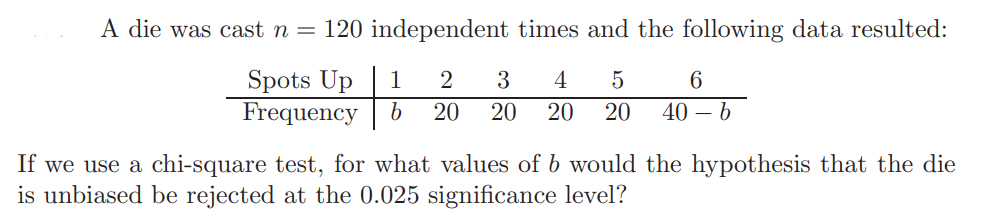
\includegraphics[scale=0.5]{474}
\end{figure}



\noindent \textit{Solution:} The test statistic under the null hypothesis $H_0: \p_i = 1/6 \forall i$ is 
\begin{align}
\chi = \sum^6_{i=1}\f{(\text{Freq}_i - 20)^2}{20} = \f{(b-20)^2}{20} + 4\cdot 0 + \f{(40-b-20)^2}{20}=\f{(b-20)^2}{10}.
\end{align}
Under the null hypothesis, $\chi \sim \chi^2(df = 5)$. At $\alpha = 0.025$, we reject the null hypothesis whenever $\chi \geq \texttt{qchisq(1-0.025,5)} = 12.8325$, i.e.,
\begin{align}
\f{(b-20)^2}{10} \geq 12.8325 \implies \boxed{b \leq 8 \lor b \geq  32}
\end{align}
\qed


















\newpage
\noindent\textbf{4.7.5} 
\begin{figure}[!htb]
	\centering
	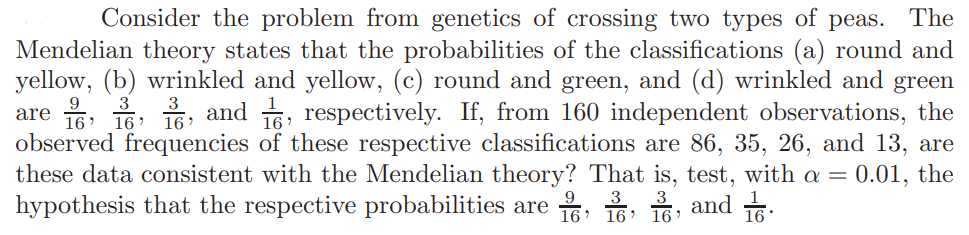
\includegraphics[scale=0.5]{475}
\end{figure}



\noindent \textit{Solution:} The test statistic under $H_0: p_a = 9/16, p_b = 3/16, p_c = 3/16, p_d = 1/16$, the test statistic is
\begin{align}
\chi = \f{(86 - 90)^2}{90} + \f{(35- 30)^2}{30} + \f{(26-30)^2}{30} + \f{(13 -10)^2}{10} = \f{22}{9}.
\end{align}
Under $H_0$, $\chi \sim \chi^2(df = 4-1 = 3)$. The p-value for this $\chi$ is $\texttt{1-pchisq(22/9, 3) = 0.4854149} > 0.01$. So, we don't have enough evidence to reject $H_0$, i.e. the data is consistent with the Mendelian theory. \qed











\newpage
\noindent\textbf{4.7.6}
\begin{figure}[!htb]
	\centering
	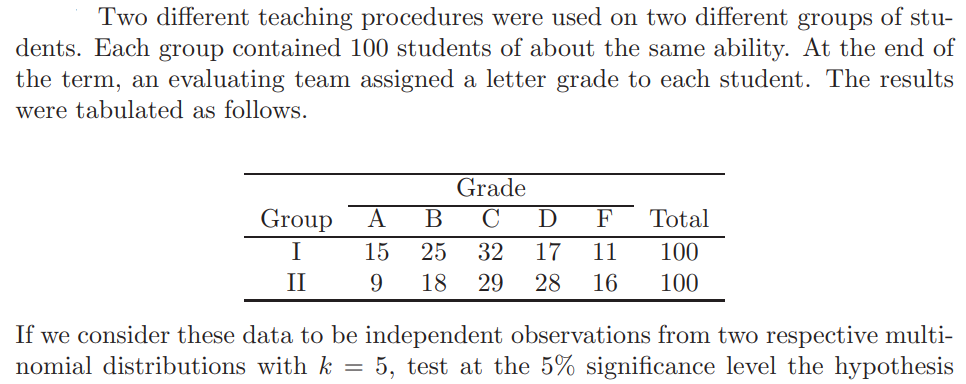
\includegraphics[scale=0.5]{476a}
	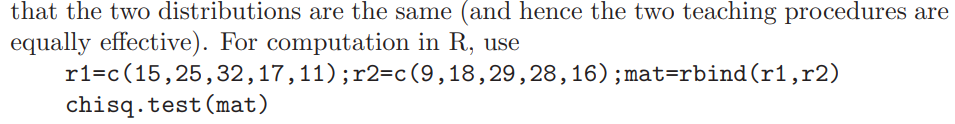
\includegraphics[scale=0.5]{476b}
\end{figure}



\noindent \textit{Solution:} Using the code provided by the problem we get
\begin{lstlisting}
> r1=c(15,25,32,17,11);r2=c(9,18,29,28,16);mat=rbind(r1,r2)
> chisq.test(mat)

Pearson's Chi-squared test

data:  mat
X-squared = 6.4019, df = 4, p-value = 0.1711
\end{lstlisting}
Since $p = 0.1711 > 0.05$, we don't have enough evidence to reject $H_0$, i.e. the two teaching procedures are (statistically) equally effective.\qed 

















\newpage
\noindent\textbf{4.8.9} (use acceptance sampling)
\begin{figure}[!htb]
	\centering
	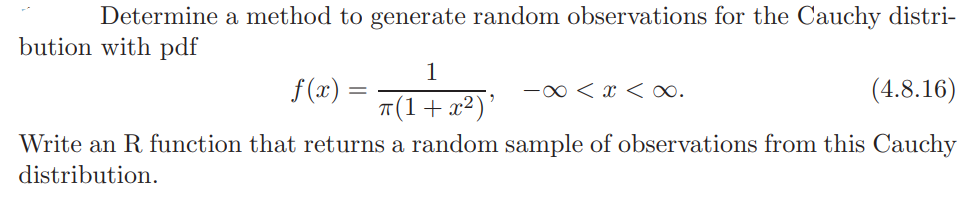
\includegraphics[scale=0.5]{489}
\end{figure}



\noindent \textit{Solution:}  \textbf{R code:}
\begin{lstlisting}
# acceptance sampling
# approximate the Cauchy distribution

x <- runif(100000,-7,7)
y <- runif(100000,0,1)

z <- cbind(x,y)
accept <- NULL
reject <- NULL

dens <- function(x){
	d <- 1/((pi^2)*(x^2+1))
	return(d)}

for (i in 1:length(x)){
	d <- dens(x[i])
	if (y[i] < d) {
		accept <- rbind(accept,z[i,])}
	else{
		reject <- rbind(reject,z[i,])}
}
# plot accepted values in red
plot(accept[,1],accept[,2], 
main = "Approximated Distribution", ylim=c(0,1), col="red")

# plot rejected values in blue
points(reject[,1], reject[,2], col = "dark blue")
\end{lstlisting}

Here's a small sample:
\begin{lstlisting}
> accept
x            y
[1,] -0.2257702402 8.676955e-02
[2,] -0.3536258731 6.871887e-02
[3,]  4.1498403600 4.068073e-03
[4,] -0.3986396971 3.033239e-02
[5,]  0.7077048477 1.492551e-02
[6,] -0.0422784868 1.612575e-02
[7,] -0.6391186416 1.029603e-02
[8,]  0.4845524384 6.119987e-02
[9,]  0.3572320105 2.479371e-02
.
.
.
\end{lstlisting}

\newpage


\begin{figure}[!htb]
	\centering
	\includegraphics[scale=0.6]{Cauchy}
\end{figure}

\qed
















\newpage
\noindent\textbf{4.8.10} (use inverse transformation sampling)
\begin{figure}[!htb]
	\centering
	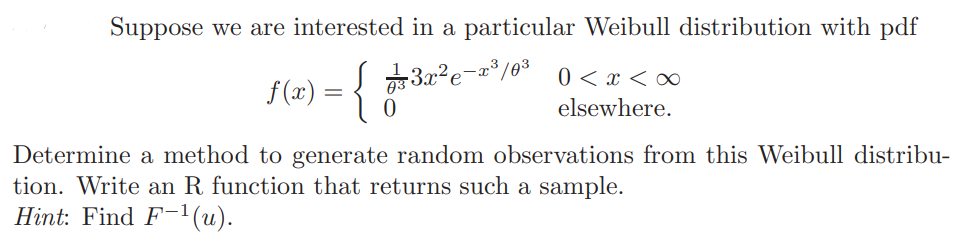
\includegraphics[scale=0.5]{4810}
\end{figure}



\noindent \textit{Solution:}  We first want to find the cdf $F$, given $f(x)$. Well, 
\begin{align}
F(x) = \int^x_{-\infty} f(x')\,dx' = \int^x_0 \f{1}{\theta^3}3x'^2 e^{-x'^3/\theta^3}\,dx' = \dots = 1 - e^{-x^3/\theta^3}.
\end{align}
With this, let $u \sim U(0,1)$ then 
\begin{align}
F^{-1}(u) = \sqrt[3]{-\theta^3\ln(1-u)} \sim \text{Wei}(k=3, \theta), \quad 0 \leq u \leq 1.
\end{align} 

Suppose $\theta = 2$ then in R, we do the following:
\begin{lstlisting}
# inverse transformation sampling
# generate vector of random uniform(0,1)
u <- runif(100000)

# set beta and transform to random weibull(shape=3, scale=theta)
beta = 2
x <- (-(beta^3)*log(1 - u))^(1/3)
hist(x, main="Histogram of Tranformed Variable", pr = TRUE)

# overlay weibull
curve(dweibull(x, shape = 3, scale=2), 
col="darkgreen", lwd=3, add=TRUE)
\end{lstlisting}

Here's a sample:
\begin{lstlisting}
> x <- (-(beta^3)*log(1 - u))^(1/3)
> x
1.57511912 1.81610458 2.51359811 1.12564398 1.21991006
1.10365173 0.71966428 2.06591082 3.08423326 1.67620145
1.02533405 1.24429387 0.94192313 2.19097666 1.98069305
0.43007645 1.18581709 1.11303036 1.63002049 2.37205273
2.45962833 1.67162606 1.61624974 1.46149955 1.92907758
1.12735030 1.02997348 2.25870529 1.58137215 2.71199084
1.05306668 1.43121600 1.17977939 1.24985669 2.22292333
1.86914252 3.01206737 1.11948037 1.64757666 1.35904188
1.39351092 2.60002179 1.12125772 2.15576011 2.41963279
\end{lstlisting}

\newpage

\begin{figure}[!htb]
	\centering
	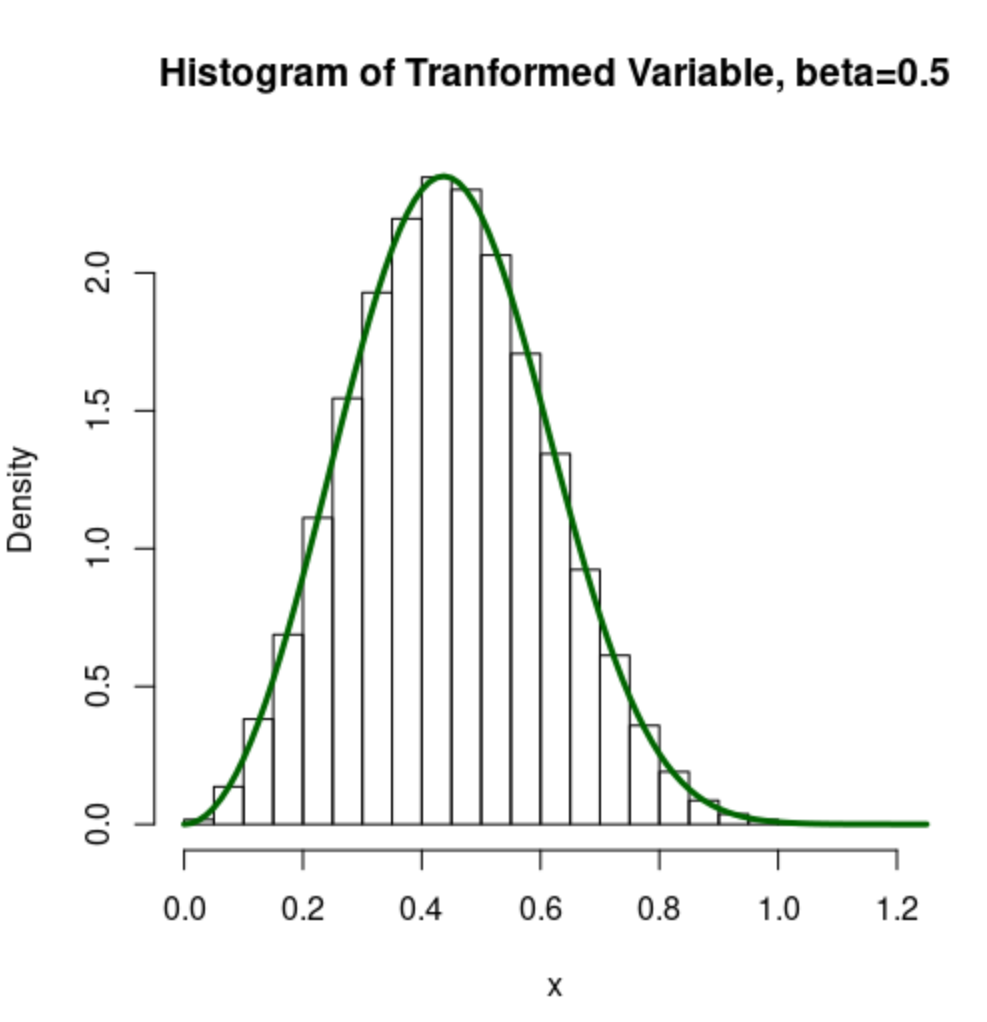
\includegraphics[scale=0.5]{beta-0-5}
	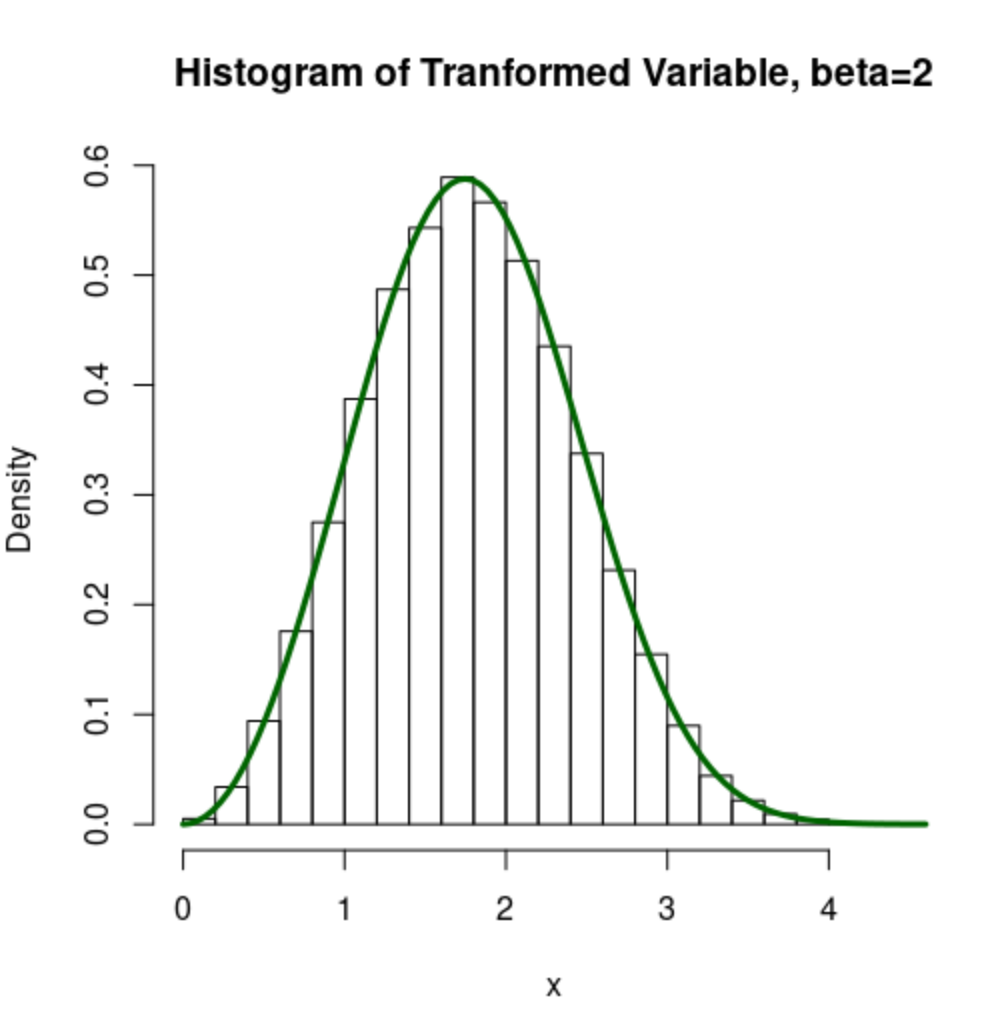
\includegraphics[scale=0.5]{beta-2}
\end{figure}\qed




\newpage























\section{Problem set 4}

\noindent\textbf{4.9.4} (for part B, write your own R function to generate the bootstrap distribution of the median -
using the code posted on Moodle is an okay starting point)

\begin{figure}[!htb]
	\centering
	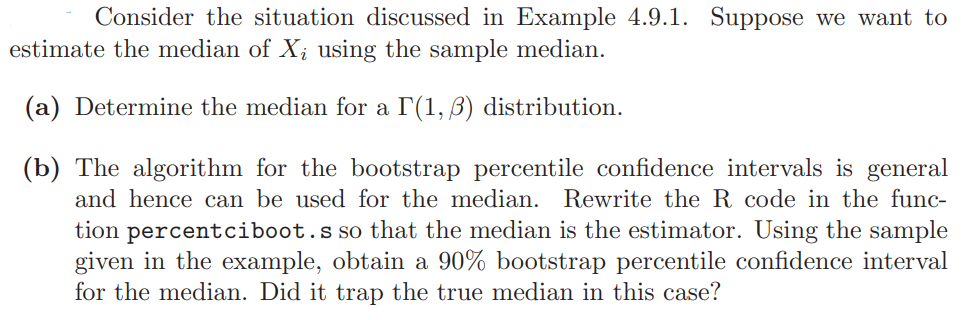
\includegraphics[scale=0.5]{494}
\end{figure}



\noindent \textit{Solution:} 


\begin{enumerate}[(a)]
	\item The median $x_{1/2}$ for a $\Gamma(1,\beta)$ is such that
	\begin{align}
	\f{1}{2} = \int^{x_{1/2}}_0 \f{1}{\beta} e^{-x/\beta} = 1 - e^{-x_{1/2}/\beta} \implies \boxed{x_{1/2} = \beta \ln(2)}
	\end{align}
	
	
	\item Here's the R code (I'm not using Prof. O'Brien's code here)
	\begin{lstlisting}
	> x <- c(131.7, 182.7, 73.3, 10.7, 150.4, 42.3, 22.2, 17.9, 264.0,
	154.4, 4.3, 265.6, 61.9, 10.8, 48.8, 22.5, 8.8, 150.6, 103.0, 85.9)
	> percentciboot <- function(x,b,alpha){
	+   theta=median(x); thetastar=rep(0,b); n=length(x)
	+   for(i in 1:b){xstar=sample(x,n,replace=T)
	+   thetastar[i]=median(xstar)}
	+   thetastar=sort(thetastar); pick=round((alpha/2)*(b+1))
	+   lower=thetastar[pick]; upper=thetastar[b-pick+1]
	+   list(theta=theta,lower=lower,upper=upper)}
	> percentciboot(x,3000,.10)
	
	$theta
	[1] 67.6
	
	$lower
	[1] 30.1
	
	$upper
	[1] 131.7
	
	> median(x)
	[1] 67.6
	
	> 100*log(2)
	[1] 69.31472
	\end{lstlisting}
	The 90\% bootstrap percentile CI for the median is given by $(30.1, 131.7)$. The true median is given by $\beta ln(2) = 100 \ln(2)  \approx 69.31472$. So, yes, the 90\% CI traps the true median in this case.
	
	
	
\end{enumerate}\qed






















\newpage
\noindent\textbf{4.9.11}


\begin{figure}[!htb]
	\centering
	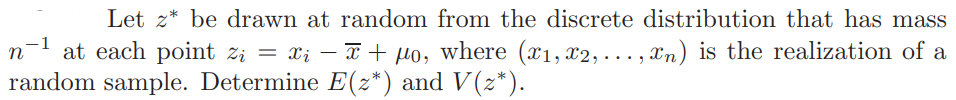
\includegraphics[scale=0.5]{4911}
\end{figure}



\noindent \textit{Solution:} 

\begin{enumerate}[(a)]
	\item $E(z^*)$:
	\begin{align}
	E(z^*) = \sum^n_{i=1}\f{x_i - \bar{x} + \mu_0}{n} = \bar{x} - \bar{x}+\mu_0 = \boxed{\mu_0}
	\end{align}
	
	\item $V(z^*)$:
	\begin{align}
	V(z^*) = \sum^n_{i=1}(z_i - E(z^*))^2 = \sum^n_{i=1}(x_i - \bar{x}+\mu_0 - \mu_0)^2 = \boxed{\sum^n_{i=1}(x_i - \bar{x})^2}
	\end{align}
\end{enumerate}\qed




















\newpage
\noindent\textbf{4.9.13}

\begin{figure}[!htb]
	\centering
	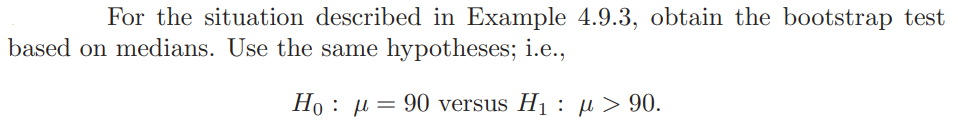
\includegraphics[scale=0.5]{4913}
\end{figure}



\noindent \textit{Solution:} Here's the R code:
\begin{lstlisting}
> X <- c(119.7, 104.1, 92.8, 85.4, 108.6, 93.4, 67.1, 88.4, 101.0, 97.2,
+        95.4, 77.2, 100.0, 114.2, 150.3, 102.3, 105.8, 107.5, 0.9, 94.1)
> boottestonemed <-
+   function(x,theta0,b){
+     #
+     #  x = sample
+     #  theta0 is the null value of the mean
+     #  b is the number of bootstrap resamples
+     #
+     #  origtest contains the value of the test statistics 
+     #           for the original sample
+     #  pvalue is the bootstrap p-value
+     #  teststatall contains the b bootstrap tests
+     #
+     n<-length(x)
+     v<-median(x)
+     z<-x-median(x)+theta0
+     counter<-0
+     teststatall<-rep(0,b)
+     for(i in 1:b){xstar<-sample(z,n,replace=T)
+     vstar<-median(xstar)
+     if(vstar >= v){counter<-counter+1}
+     teststatall[i]<-vstar}
+     pvalue<-counter/b
+     list(origtest=v,pvalue=pvalue,teststatall=teststatall)
+     #list(origtest=v,pvaule=pvalue)
+   }
> boottestonemed(X,90,3000)
$origtest
[1] 98.6

$pvalue
[1] 0.006
\end{lstlisting}

At such a low p-value ($p = 0.006$), we reject the null hypothesis $H_0$. So even though we don't reject $H_0$ with the test based on sampling mean, we \textit{do} reject $H_0$ with the test based on medians. \qed


















\newpage




\noindent \textbf{5.1.7}


\begin{figure}[!htb]
	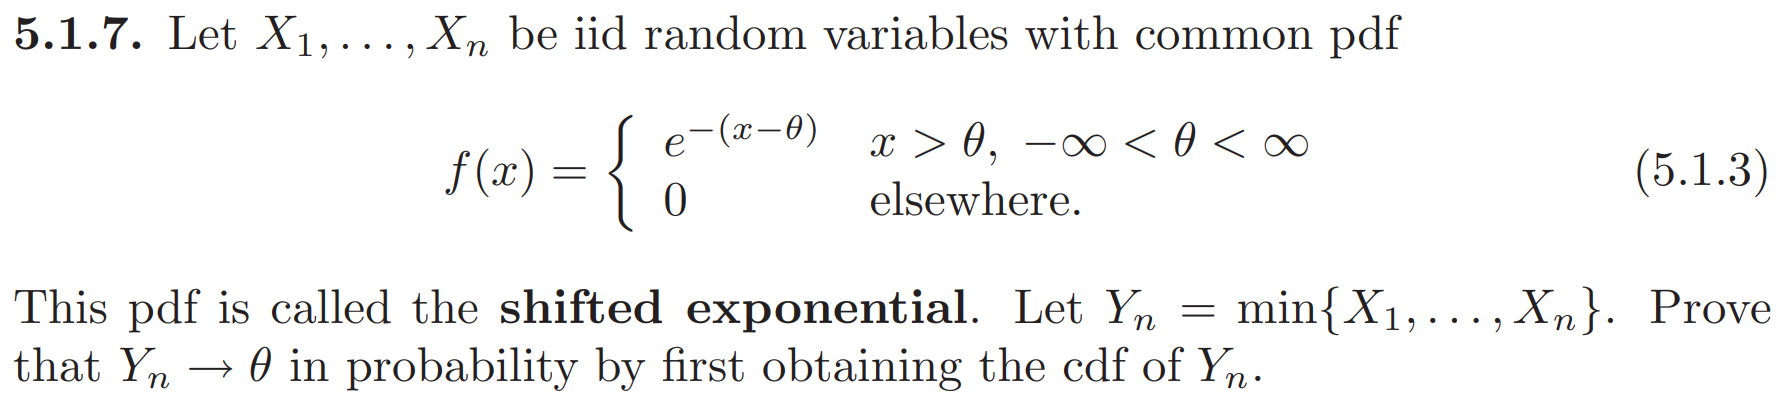
\includegraphics[scale=0.25]{517}
\end{figure}



\noindent \textit{Solution:} By definition,
\begin{align}
Y_n \xrightarrow{P} \theta &\iff \forall \epsilon > 0, \lim_{n\to \infty}P[\abs{Y_n - \theta} \geq \epsilon ] = 0\nn\\
&\iff \forall \epsilon > 0, \lim_{n\to \infty}P[\abs{\min\{ X_1,\dots,X_n\} - \theta} \geq \epsilon ] = 0\nn\\
&\iff \forall \epsilon > 0, \lim_{n\to \infty}P[\min\{ X_1,\dots,X_n\} - \theta \geq \epsilon] = 0\nn\\
&\iff \forall \epsilon > 0, \lim_{n\to \infty}P[Y_n  \geq \epsilon+\theta] = 0
\end{align}
where the second to last equivalence statement comes from the fact that $x_i > \theta\, \forall i = 1,2,\dots,n$. To show $Y_n \xrightarrow{P} \theta$, we find the cdf for $Y_n$:
\begin{align}
F_{Y_n}(y) &= P(Y_n < y)\nn\\
&= 1- P(Y_n \geq y_m)\nn\\
&= 1 - \prod^n_{i=1}P(X_i \geq y)\nn\\
&= 1 - \prod^n_{i=1}\int^\infty_{y} e^{-(x-\theta)}\,dx\nn\\
&= 1 - \prod^n_{i=1} e^{-(y - \theta)}\nn\\
&= 1 - e^{-n(y - \theta)}\nn\\
P(Y_n \geq y) &= e^{-n(y - \theta)}.
\end{align}
Let $\epsilon > 0$ be given. Then 
\begin{align}
P(Y_n \geq \epsilon+\theta) = e^{-n(\epsilon + \theta - \theta)} = e^{-n\epsilon},
\end{align}
and so 
\begin{align}
\lim_{n\to \infty}P[\abs{Y_n - \theta} \geq \epsilon ] = \lim_{n\to \infty}P[Y_n  \geq \epsilon+\theta] = \lim_{n\to \infty} e^{-n\epsilon} = 0 \implies Y_n \xrightarrow{P} \theta.
\end{align}\qed



\newpage


\noindent \textbf{5.2.2} (Investigate = find)

\begin{figure}[!htb]
	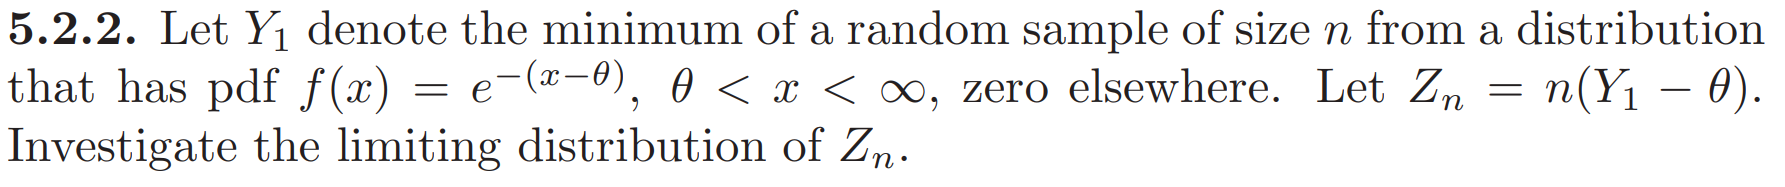
\includegraphics[scale=0.25]{522}
\end{figure}

\noindent \textit{Solution:} Let $F_{Z_n}$ and $F_Z$ be, respectively, the cdfs of $Z_n$ and $Z$. Then by definition 
\begin{align}
Z_n \xrightarrow{D} Z \iff \lim_{n\to \infty} F_{Z_n}(z) = F_Z(z)
\end{align}
for all $z$ at which $F_Z(z)$ is continuous. Now, we don't know what $F_Z$ is in this case, but we can find what $F_{Z_n}$ converges to when $n\to \infty$. To show this, we find $F_{Z_n}$:
\begin{align}
F_{Z_n}(z) &= P(Z_n \leq z)\nn\\
&= P(n(Y_1 - \theta) \leq z)\nn\\
&= P(Y_1 \leq z/n + \theta)\nn\\
&= 1 - e^{-n(z/n+ \theta - \theta)}, \quad \text{calculated in Problem 5.1.7}\nn\\
&= 1 - e^{-z}.
\end{align}
And so (obviously)
\begin{align}
\lim_{n\to \infty} F_{Z_n}(z) = 1 - e^{-z} \equiv \text{cdf}(\text{Exp}(1))
\end{align}
Therefore, $Z_n \xrightarrow{D} Z \sim \text{Exp}(1)$.\qed



\newpage




\noindent \textbf{5.2.7}

\begin{figure}[!htb]
	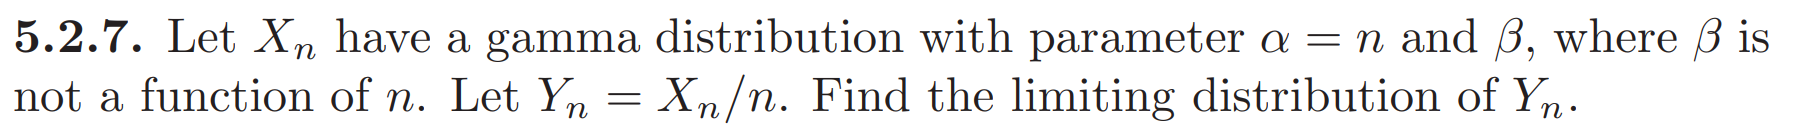
\includegraphics[scale=0.25]{527}
\end{figure}


\noindent \textit{Solution:} Let $X_n \sim \Gamma(\al = n, \be)$ be given, where $\be$ is not a function of $n$. Let $Y_n = X_n/n$. To find the limiting distribution of $Y_n$, we find $\lim_{n\to \infty} M_{Y_n}(t)$. The reason we don't want to find the cdf $F_{Y_n}$ is that integrals involving the Gamma distribution are often ugly.
\begin{align}
M_{Y_n}(t) &= E[e^{tY_n}] =  E[e^{tX_n/n}] \equiv E[e^{t_n X_n}] \nn\\
&= (1 - \be t_n)^{-n}\nn\\
&= \lp 1 - \f{\beta t}{n} \rp^{-n}.
\end{align}
And so using the identity 
\begin{align}
\lim_{n\to \infty} \lp 1- \f{1}{n} \rp^{-n} = e,
\end{align}
by change of variables we obtain
\begin{align}
\lim_{n\to \infty}M_{Y_n}(t) = \lim_{n\to \infty} \lp 1 - \f{\beta t}{n} \rp^{-n} = e^{\be t} 
\end{align}
So what is the limiting distribution of $Y_n$? By definition,
\begin{align}
M_Y(t) = E[e^{tY}] = \int_\infty^\infty f_Y(y)e^{yt}\,dy  = e^{\beta t}.
\end{align}
Upon inspection, this equality holds if and only if $f_Y(y) \equiv \delta(y-\beta)$, the delta function centered at $\beta$. 
\begin{align}
\int^\infty_{-\infty} \delta(y-\beta)e^{yt}\,dy = e^{\beta t}.
\end{align}
And so, the limiting distribution of $Y_n$ is the degenerate distribution with parameter $\beta$:
\begin{align}
Y_n \xrightarrow{D} Y \sim \delta(y - \beta) \equiv \begin{cases}
1, \quad y = \beta\\
0, \quad \text{else}
\end{cases}.
\end{align}
\qed












\newpage



\noindent \textbf{5.3.9}

\begin{figure}[!htb]
	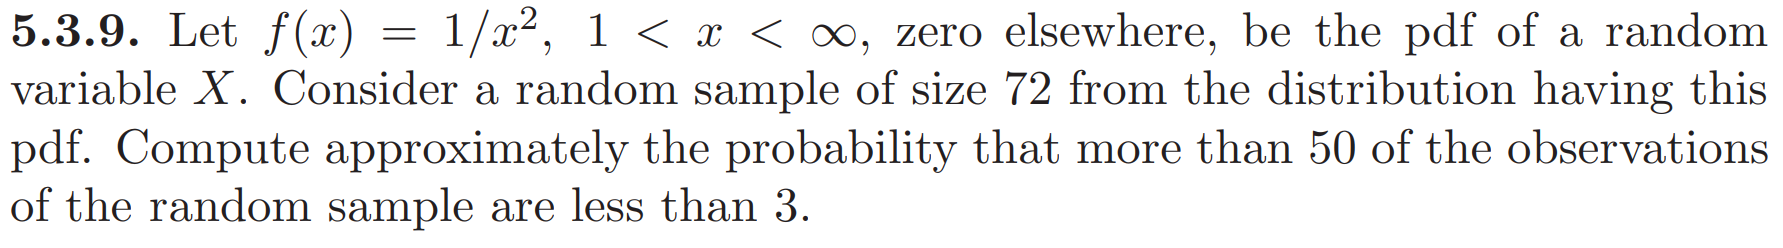
\includegraphics[scale=0.25]{539}
\end{figure}


\noindent \textit{Solution:} We have $X_1, \dots, X_{72}$, with 
\begin{align}
X_i \sim f(x) = \begin{cases}
\f{1}{x^2}, \quad 1 < x < \infty\\
0, \quad \text{else}
\end{cases}.
\end{align}
We first find the probability that any given observation is less than 3:
\begin{align}
P(X < 3) = \int_1^3 \f{1}{x^2}\,dx = \f{2}{3}.
\end{align}
So we have a ``binomial situation'' where the probability of success is $p=2/3$. Given $n=72$ trials, we have $\mu = np = 72(2/3) = 48$ and $\sigma = \sqrt{np(1-p)} = 4$. We wish to find the probability of having more than 50 successes. To this end, we use the normal approximation (CLT), which says
\begin{align}
\f{Y_{72} - \mu}{\sigma} \sim \N(0,1).
\end{align}
And so
\begin{align}
P(Y_{72} > 50) &\approx P\lp Z \geq \f{51 - 48}{4}  \rp\nn\\
&= \texttt{1-pnorm(3/4)}\nn\\
&= \boxed{0.2266274}
\end{align}
Or we can also use the continuity correction to get
\begin{align}
P(Y_{72} > 50) &\approx P\lp Z \geq \f{50.5 - 48}{4}  \rp\nn\\
&= \texttt{1-pnorm((50.5-48)/4)}\nn\\
&= \boxed{0.2659855}
\end{align}
\qed












\newpage




\noindent \textbf{5.3.11}
\begin{figure}[!htb]
	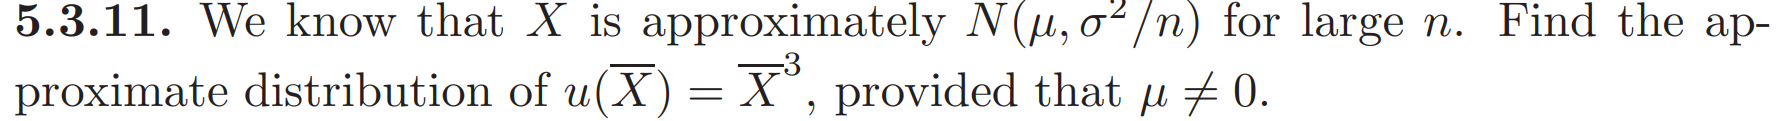
\includegraphics[scale=0.25]{5311}
\end{figure}



\noindent \textit{Solution:} We want to use the $\Delta$-method for this problem. Since $\bar{X} \sim \N(\mu, \sigma^2/n)$, we have
\begin{align}
\sqrt{n}(\bar{X} - \mu) \xrightarrow{D} \N(0,\sigma^2),
\end{align}
by a simple change of variables. The function $u(\bar{X}) = \bar{X}^3$ is differential at for all $\bar{X}$ and $u'(\bar{X}) \neq 0$ in general, so by the $\Delta$-method,
\begin{align}
&\sqrt{n}(u(\bar{X}) - u(\mu)) \xrightarrow{D} \N(0, \sigma^2(u'(\mu))^2)\nn\\
\iff &\sqrt{n}(u(\bar{X}) - u(\mu)) \xrightarrow{D} \N(0, \sigma^2(3\mu^2)^2)\nn\\
\iff &\sqrt{n}(u(\bar{X}) - \mu^3) \xrightarrow{D} \N(0, 9\sigma^2\mu^4).
\end{align}
\noindent But of course, the convergence in distribution above is equivalent to 
\begin{align}
u(\bar{X}) = \bar{X}^3 \xrightarrow{D} \N\lp\mu^3, \f{9\sigma^2\mu^4}{n} \rp,
\end{align}
again by change of variables. \qed




\newpage




\section{Problem set 5}


\noindent \textbf{6.1.1}
\begin{figure}[!htb]
	\centering
	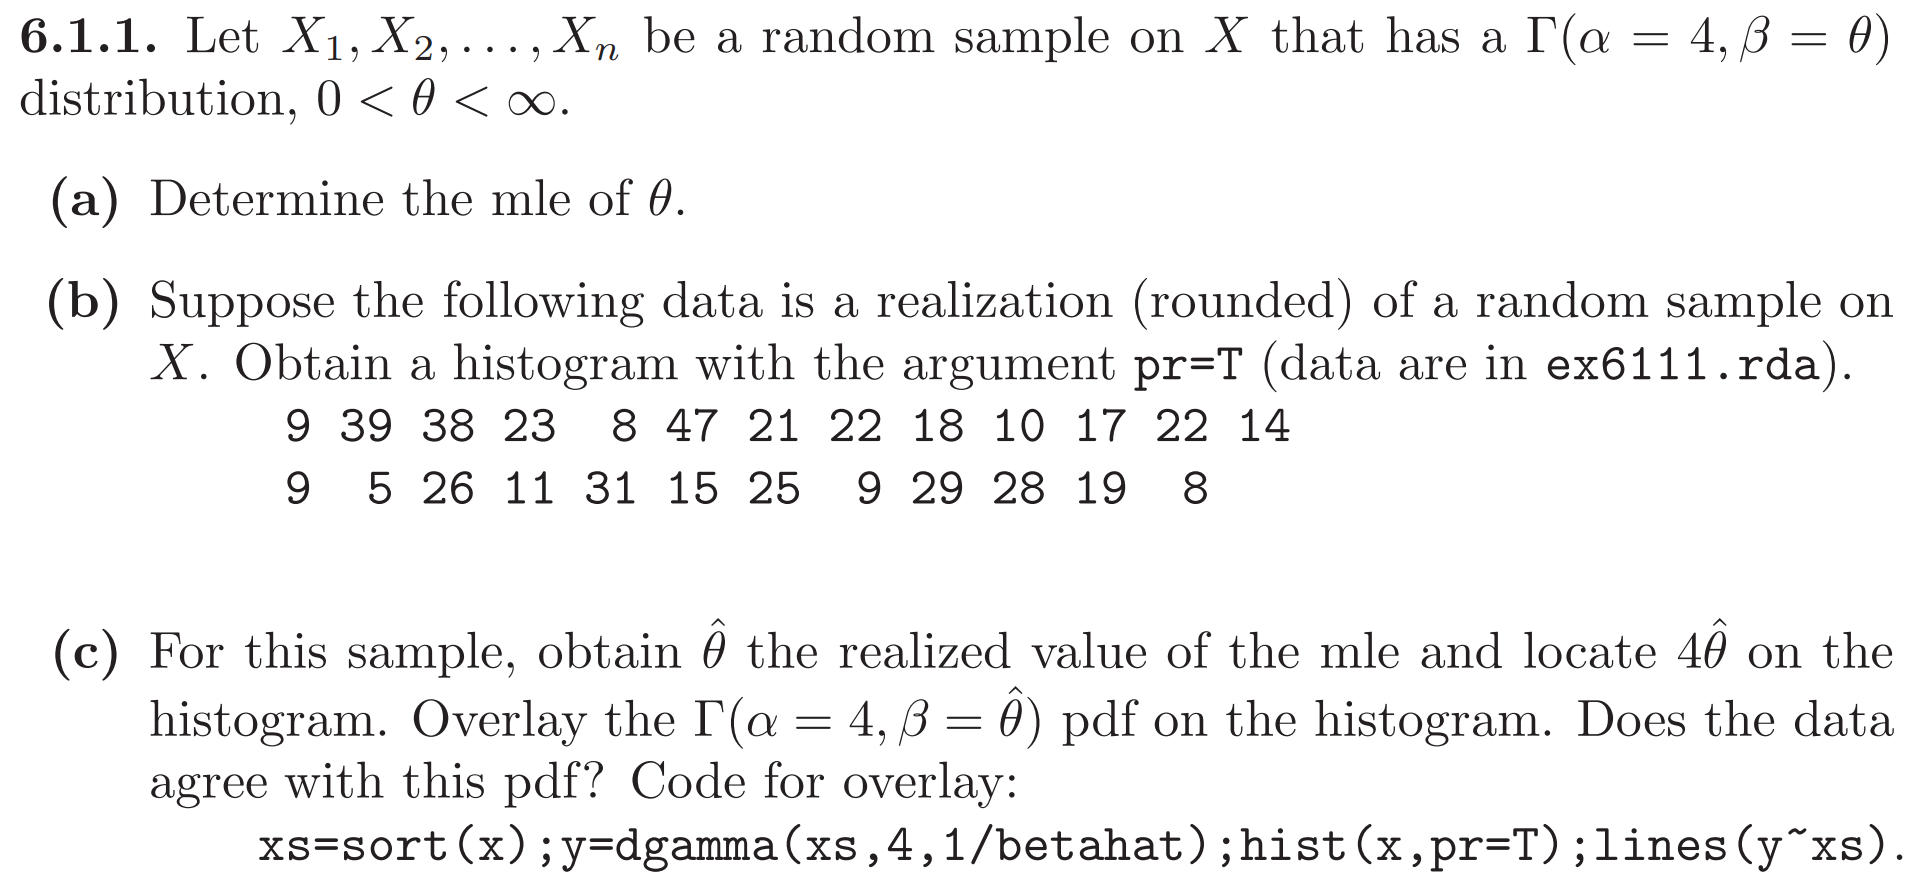
\includegraphics[scale=0.25]{611}
\end{figure}
 
 
 
\noindent \textit{Solution:} 
\begin{enumerate}[(a)]
	\item The likelihood function is 
	\begin{align}
	\lag(\theta) = \prod^n_{i=1} \f{1}{\Gamma(4) \theta^{4}} x_i^{4-1}e^{-\theta x_i} = \f{1}{\Gamma(4)^n} \f{1}{\theta^{4n}} e^{- \sum^n_{i=1} x_i/\theta} \prod^n_{i=1} x_i^3.
	\end{align}
	The log likelihood function is then 
	\begin{align}
	l(\theta) = -n \ln (\Gamma(4)) -4n \ln \theta -\f{1}{\theta} \sum^n_{i=1}x_i + \ln \lp \prod^n_{i=1}x_i^3 \rp.
	\end{align}
	Next, solve for $\p_\theta l(\theta) = 0$:
	\begin{align}
	\p_\theta l(\theta) = -\f{4n}{\theta} + \f{1}{\theta^2} \sum^n_{i=1}x_i = 0 \iff \boxed{\hat{\theta}_{ML} = \f{1}{4n}\sum^n_{i=1}x_i = \f{\bar{x}}{4}}
	\end{align}
	
	\item 
	\textbf{R code:}
	\begin{lstlisting}
	> dat = c(9, 39, 38, 23, 8 ,47 ,21, 22, 18, 10, 17, 22, 14, 
	+         9, 5, 26, 11, 31, 15, 25, 9, 29, 28, 19, 8)
	> hist(dat, pr=T)
	\end{lstlisting}
	\begin{figure}[!htb]
		\centering
		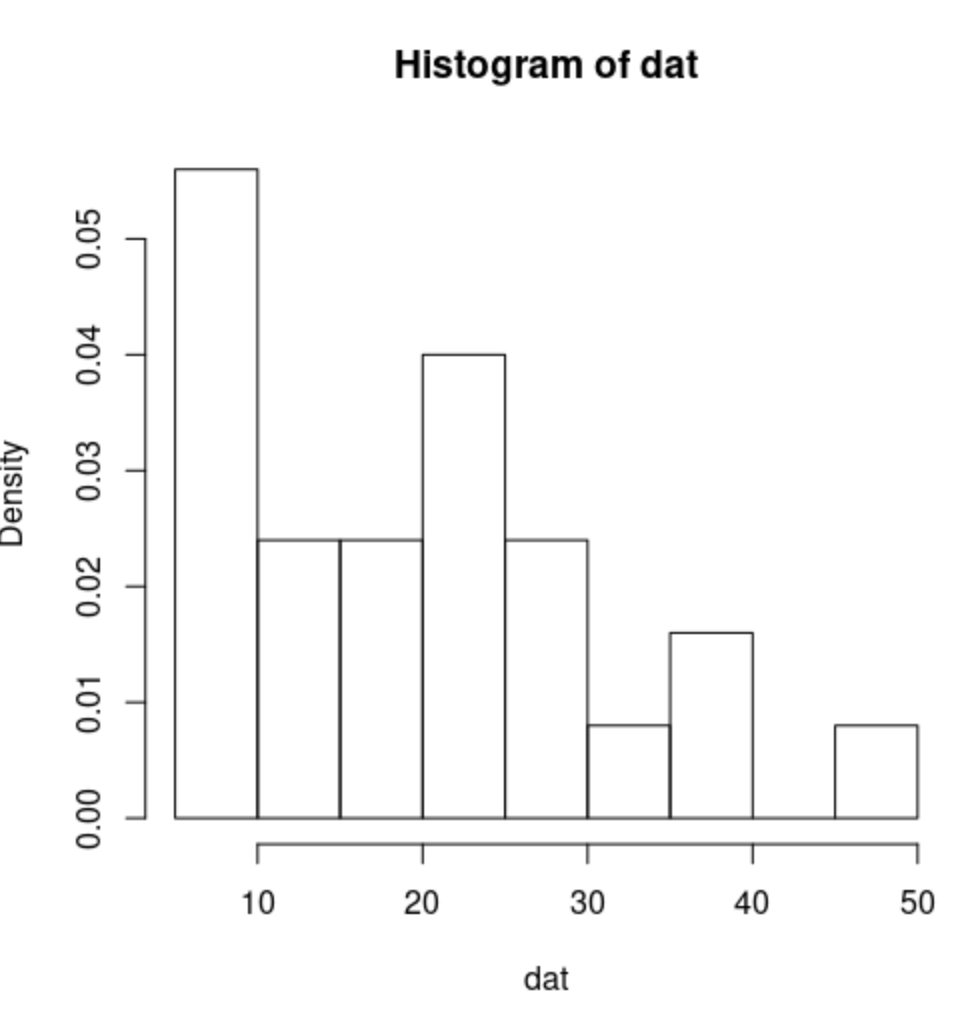
\includegraphics[scale=0.2]{dat611}
		\caption{(b)}
	\end{figure}
	
	
	
	\newpage
	
	\item $\boxed{\hat\theta = \bar{x}/4 = 5.03}$ \textbf{R code:}
	\begin{lstlisting}
	> mean(dat)/4
	[1] 5.03
	
	> xs=sort(dat)
	> y=dgamma(xs,4,4/mean(dat))
	> hist(dat,pr=T)
	> lines(y~xs)
	\end{lstlisting}
	Locate $4\hat\theta$ on the histogram and overlay with $\Gamma(\alpha =4, \be = \hat\theta = 5.03)$:
	\begin{lstlisting}
	> xs=sort(dat)
	> y=dgamma(xs,4,4/mean(dat))
	> hist(dat,pr=T)
	> lines(y~xs)
	> abline(v=mean(dat))
	\end{lstlisting}
	\begin{figure}[!htb]
		\centering
		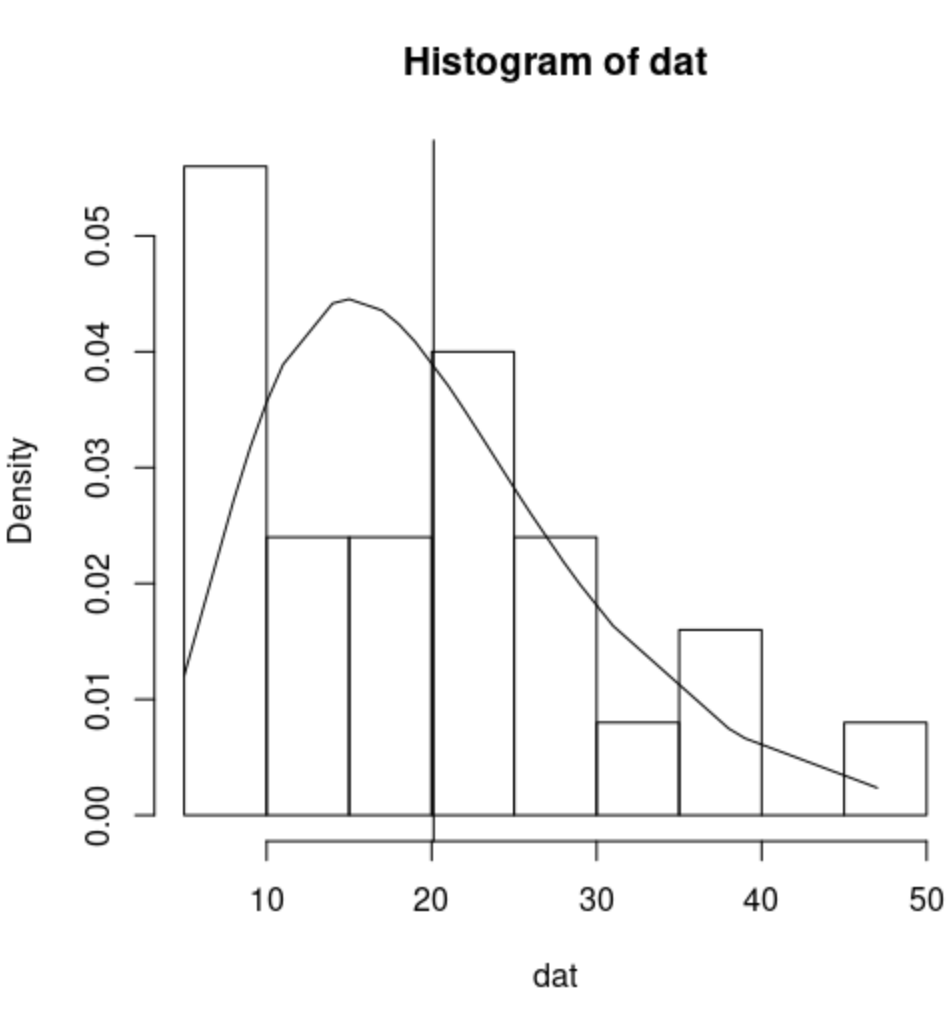
\includegraphics[scale=0.2]{dat611a}
	\end{figure}
	The data somewhat agrees with this pdf. 
	
\end{enumerate}

\qed












\newpage
\noindent \textbf{6.1.2}
\begin{figure}[!htb]
	\centering
	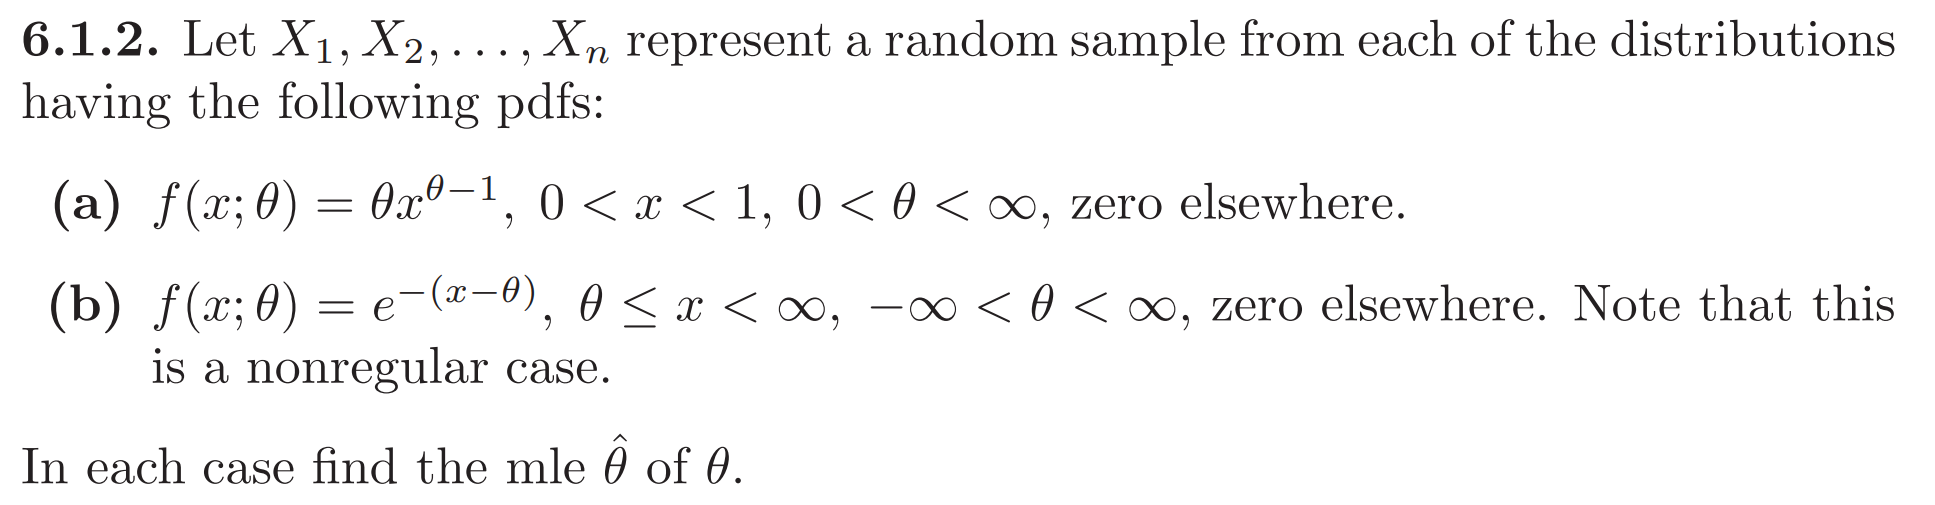
\includegraphics[scale=0.25]{612}
\end{figure}


\noindent \textit{Solution:} 
\begin{enumerate}[(a)]
	\item The likelihood function is 
	\begin{align}
	\lag(\theta) = \theta^n \prod^n_{i=1} x_i^{\theta - 1}, \quad x_i \in (0,1), 0 < \theta < \infty.
	\end{align}
	The log likelihood is
	\begin{align}
	l(\theta) = \ln \lag(\theta) = n \ln \theta + (\theta - 1)\sum^n_{i=1}\ln x_i.
	\end{align}
	Then we solve for $\theta$ in $\p_\theta l(\theta) = 0$:
	\begin{align}
	\p_\theta l(\theta) = \f{n}{\theta} + \sum^n_{i=1}\ln (x_i) = 0 \implies \boxed{\hat\theta = \f{-n}{\sum^n_{i=1}\ln x_i} }
	\end{align}
	
	
	
	
	
	
	
	\item The likelihood function is 
	\begin{align}
	\lag(\theta) = e^{-\sum^n_{i=1}(x_i - \theta)}, \quad \theta < x_i < \infty, -\infty < \theta < \infty.
	\end{align}
	Then the log likelihood is
	\begin{align}
	l(\theta) = \ln \lag(\theta) = -\sum^n_{i=1} x_i + n\theta.
	\end{align}
	Next,
	\begin{align}
	\p_\theta l(\theta) = n > 0.
	\end{align}
	So, $\hat\theta$ must be as large as possible to maximize $\lag(\theta)$. But at the same time, $\theta \leq x_i$ for all $i$, so 
	\begin{align}
	\boxed{\hat\theta = \min_i (X_i)}
	\end{align}
	
	
	
\end{enumerate}


\qed






\newpage
\noindent \textbf{6.1.4}
\begin{figure}[!htb]
	\centering
	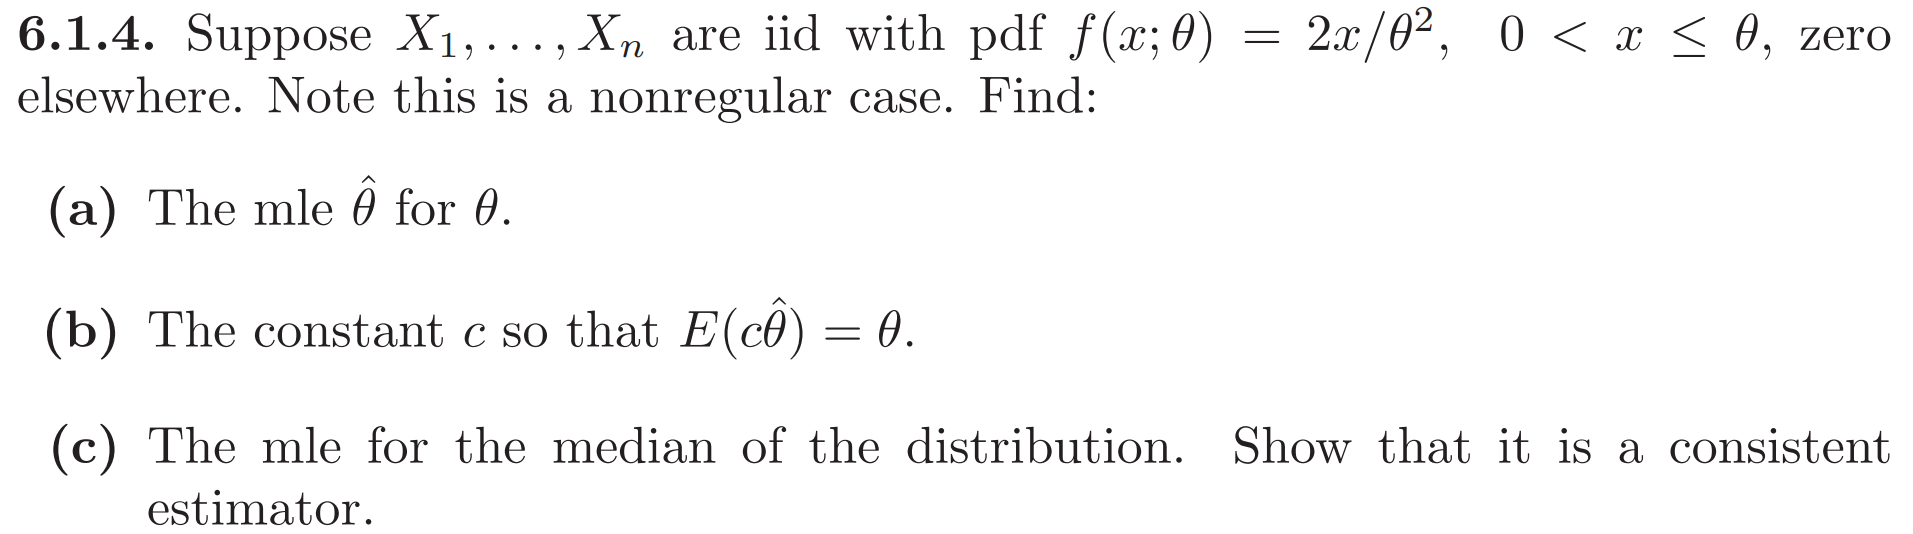
\includegraphics[scale=0.25]{614}
\end{figure}

\noindent \textit{Solution:}

\begin{enumerate}[(a)]
	\item  The likelihood function is 
	\begin{align}
	\lag(\theta) = \f{2^n}{\theta^{2n}}\prod_{i=1}^n x_i, \quad 0 < x_i \leq \theta.
	\end{align}
	The log likelihood is then 
	\begin{align}
	l(\theta) = n\ln 2 - 2n \ln \theta + \ln \lp \prod^n_{i=1} x_i \rp.
	\end{align}
	Next,
	\begin{align}
	\p_\theta l(\theta) = -\f{2n}{\theta}. 
	\end{align}
	We cannot set this to zero. However, by inspection, $\lag(\theta)$ is maximized whenever $\theta$ is minimized while $x_i \leq \theta$ for all $i$, so 
	\begin{align}
	\boxed{\hat\theta = \max(X_i) = Y_n}
	\end{align}
	
	
	\item To find $c$ we first find $E(\hat\theta)$. To get this, we must first find its cdf. 
	\begin{align}
	F_{Y_n}(x) = P(Y_n \leq x) = \prod^n_{i=1}P(x_i \leq x) = \prod^n_{i=1}F_X(x) = \f{x^{2n}}{\theta^{2n}}.
	\end{align}
	Differentiating this w.r.t. $x$ we get te pdf of $Y_n$:
	\begin{align}
	f_{Y_n}(x) = \p_x F_{Y_n}(x) = 2n \f{x^{2n - 1}}{\theta^{2n}}.
	\end{align}
	From here, calculating the expectation is easy:
	\begin{align}
	E(Y_n) = \int^\theta_0 2n \f{x^{2n-1}\cdot x}{\theta^{2n}}\,dx = \f{2n}{2n+1}\theta.  
	\end{align}
	Because we want $E(c\hat\theta) =cE(\hat\theta) = \theta$, we can just make 
	\begin{align}
	\boxed{c = \f{2n+1}{2n}}
	\end{align}
	
	
	
	
	\item The median $x_{1/2}$ is such that:
	\begin{align}
	\f{1}{2} = \int^{x_{1/2}}_0 \f{2x}{\theta^2}\,dx = \f{x^2_{1/2}}{\theta^2}.
	\end{align}
	So, $x_{1/2} = \theta/\sqrt{2}$. By the invariance property, we have
	\begin{align}
	\boxed{\hat{x}_{1/2} = \f{\hat\theta}{\sqrt{2}}}
	\end{align}
	
	Since $E(\hat\theta) = (2n+1)/2n \cdot \theta$, we see that $\lim_{n\to \infty} E(\hat\theta) = \theta$. Next, look at the variance of $\hat\theta$:
	\begin{align}
	\Var(\hat\theta) &= \Var(Y_n) = E[\hat\theta^2] - E[\hat\theta]^2 \nn\\
	& \int^\theta_0 2n \f{x^{2n-1}\cdot x^2}{\theta^{2n}}\,dx - \lp\f{2n}{2n+1}\rp^2\theta^2\nn\\
	&= \f{2n}{2+2n} \theta^2 - \lp\f{2n}{2n+1}\rp^2\theta^2.
	\end{align}
	Obviously, $\lim_{n\to \infty} 2n/(2+2n) - (2n/(2n+1))^2 = 0$, so $\lim_{n\to \infty}\Var(\hat\theta) = 0$. With this, we conclude $\hat\theta$ is a consistent estimator of $\theta$. 
	
	
	
\end{enumerate}\qed





\qed




\newpage
\noindent \textbf{6.1.10}
\begin{figure}[!htb]
	\centering
	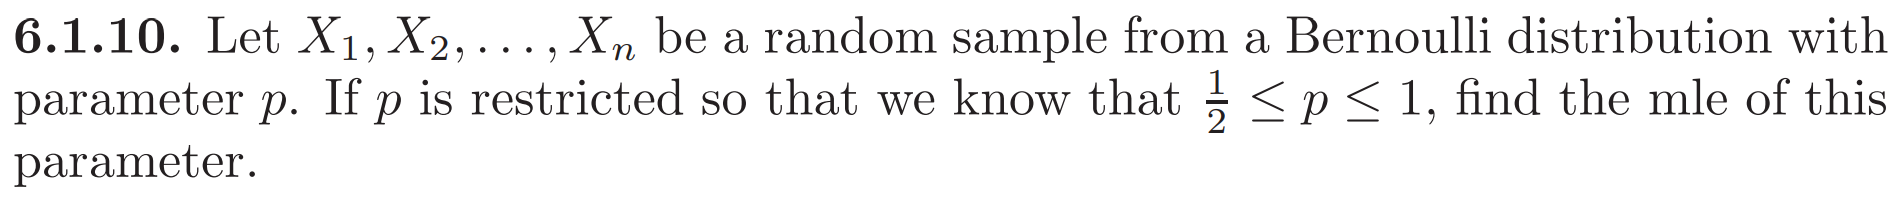
\includegraphics[scale=0.25]{6110}
\end{figure}

\noindent \textit{Solution:} The likelihood function is 
\begin{align}
\lag(x;p) = \prod^n_{i=1}f(x_i;p) = p^{\sum_{i=1}^n x_i}(1-p)^{n-\sum^n_{i=1}x_i}.
\end{align}
The log likelihood is then
\begin{align}
l(p) = \sum_{i=1}^n x_i \ln p + \lp n - \sum^n_{i=1}x_i \rp \ln (1-p).
\end{align}
Taking $\p_p$ of $l(p)$ gives
\begin{align}
\p_p l(p) = \f{\sum^n_{i=1}x_i}{p} + \f{n - \sum^n_{i=1}x_i}{1-p}.
\end{align}
Letting $\p_p l(p) = 0$, we get
\begin{align}
\hat{p} = \f{1}{n}\sum^n_{i=1}x_i = \bar{X}
\end{align}
as expected. Now, since $1/2 \leq p \leq 1$, we must consider the case where $\bar{X} < 1/2$. If $\bar{X} < 1/2$, then because $p$ cannot take the value of $\bar{X}$, it must take the boundary value of $1/2$ at which $l(p)$ is maximized. So, 
\begin{align}
\boxed{\hat{p} = \max \lp \f{1}{2},\bar{X} \rp}
\end{align}

\qed











\newpage
\noindent \textbf{6.2.2}
\begin{figure}[!htb]
	\centering
	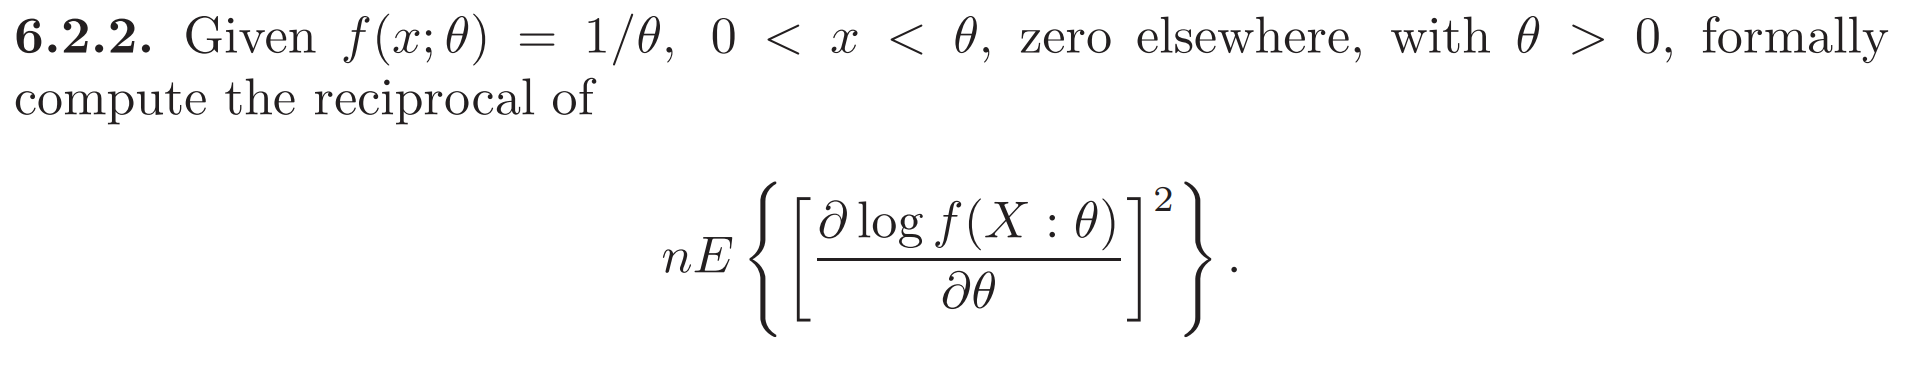
\includegraphics[scale=0.25]{622a}
	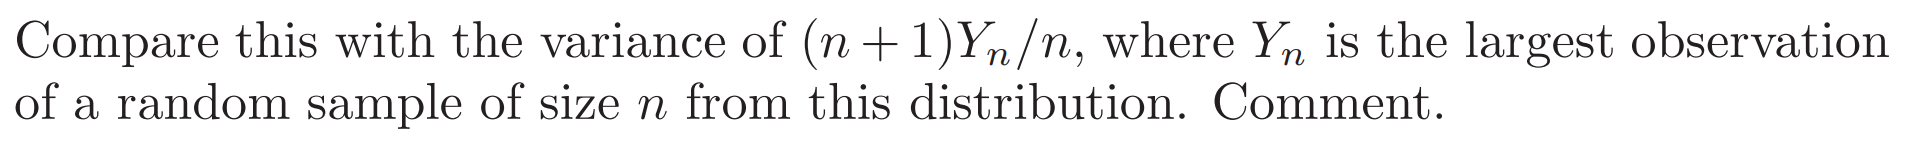
\includegraphics[scale=0.25]{622b}
\end{figure}

\noindent \textit{Solution:} 
\begin{align}
nE\lb \lp \p_\theta \ln f(x;\theta) \rp^2 \rb = nE \lb \lp \p_\theta (-\ln \theta) \rp^2 \rb = n E\lb \f{1}{\theta^2} \rb = \f{n}{\theta^2}.
\end{align}
The reciprocal of this is therefore 
\begin{align}
\f{\theta^2}{n}.
\end{align}
On the other hand,
\begin{align}
\Var\lb \f{(n+1)}{n}Y_n \rb &= \lp \f{n+1}{n} \rp^2 \lp E[Y_n^2] - E[Y_n]^2 \rp.
\end{align}
The cdf of $x$ is given by $F_X(x) = x/\theta$. The cdf of $Y_n$ is therefore 
\begin{align}
F_Y(x) = \prod^n_{i=1}F_x(x) = \f{x^n}{\theta^n} \implies f_Y(x) = n\f{x^{n-1}}{\theta^n}.
\end{align}
And so 
\begin{align}
E[Y_n] &= \int^\theta_0 n \f{x^{n-1}\cdot x}{\theta^n}\,dx = \f{n\theta}{n+1}.\\
E[Y_n^2] &= \int^\theta_0 n \f{x^{n-1}\cdot x^2}{\theta^n}\,dx = \f{n\theta^2}{n+2}.
\end{align}
So,
\begin{align}
\Var\lb \f{(n+1)}{n}Y_n \rb = \lp \f{n+1}{n} \rp^2 \lb  \f{n\theta^2}{n+2}  - \lp \f{n\theta}{n+1} \rp^2 \rb = \f{\theta^2}{n(n+2)}.
\end{align}
So, obviously,
\begin{align}
\Var[Y_n]  = \f{\theta^2}{n(n+2)} < \f{\theta^2}{n}.
\end{align}
However, since the support of $f(x;\theta)$ depends on $\theta$, CRLB does not apply. 
\qed












\newpage
\noindent \textbf{6.2.7}
\begin{figure}[!htb]
	\centering
	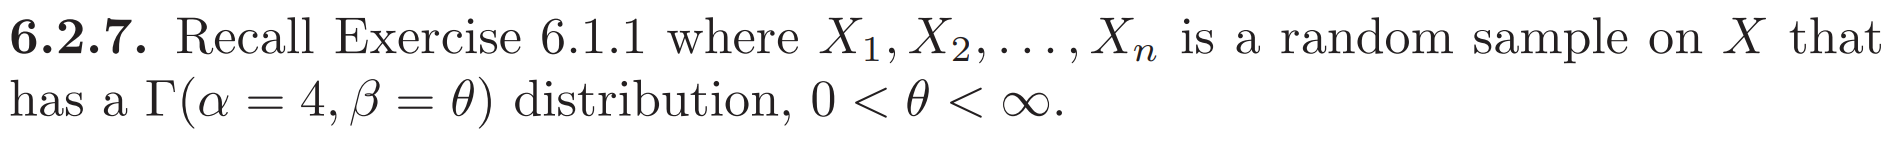
\includegraphics[scale=0.25]{627a}
	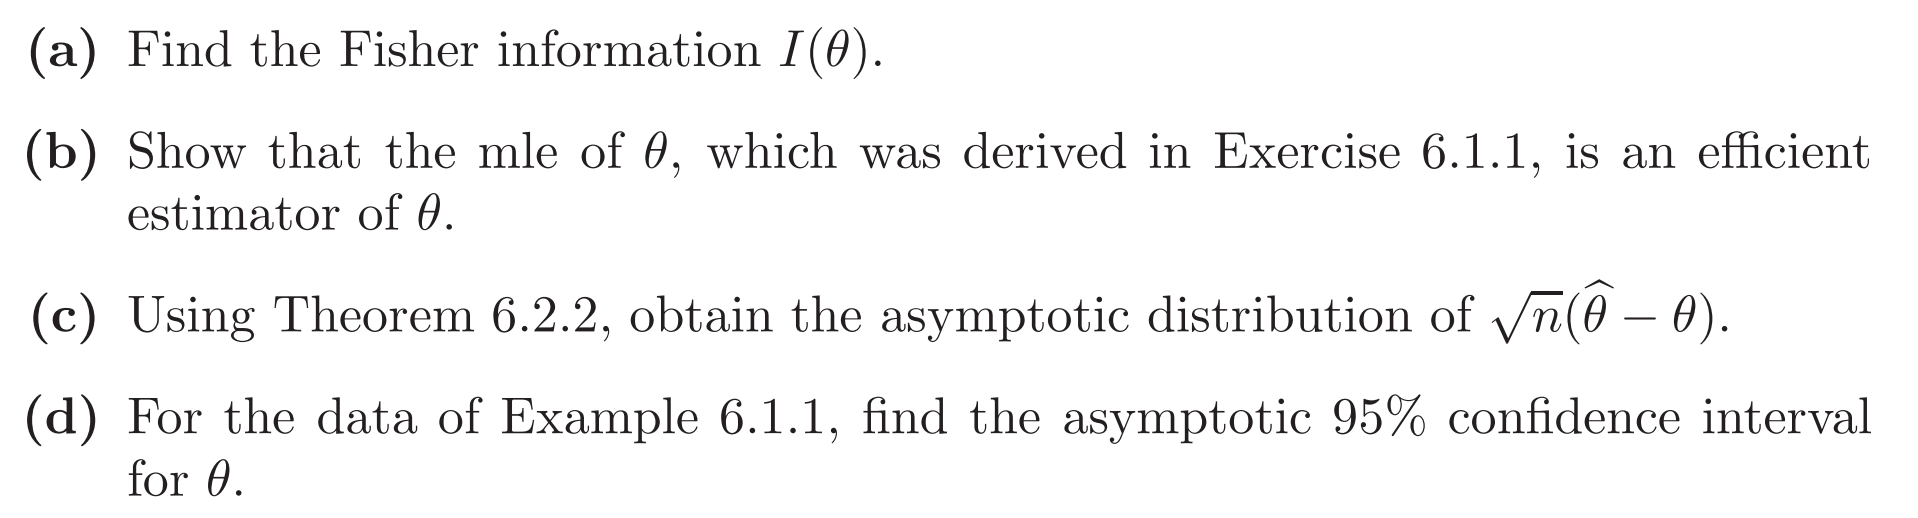
\includegraphics[scale=0.25]{627b}
\end{figure}

\noindent \textit{Solution:}


\begin{enumerate}[(a)]
	\item From 6.1.1. we know that 
	\begin{align}
	\p_\theta l(\theta) = -\f{4n}{\theta} + \f{1}{\theta^2}\sum^n_{i=1} x_i \implies \p^2_\theta l(\theta) = \f{4n}{\theta^2} - \f{2}{\theta^3}\sum^n_{i=1} x_i
	\end{align}
	And so 
	\begin{align}
	nI(\theta) 
	&= -E\lb\f{4n}{\theta^2} - \f{2}{\theta^3}\sum^n_{i=1} x_i \rb\nn\\ 
	&= -\f{4n}{\theta^2} + \f{2}{\theta^3}\sum^n_{i=1}E[x_i]\nn\\
	&= -\f{4n}{\theta^2} + \f{2}{\theta^3}n 4\theta\nn\\
	&= -\f{4n}{\theta^2} + \f{8n}{\theta^2}\nn\\
	&= \boxed{\f{4n}{\theta^2}}  \implies \boxed{I(\theta) = \f{4}{\theta^2}}
	\end{align}
	
	
	\item From 6.1.1., $\hat\theta = \bar{X}/4$, which is unbiased because 
	\begin{align}
	E[\hat\theta] = \f{1}{4}E[\bar{X}] = \f{1}{4}\f{4n\theta}{n} = \theta.
	\end{align}
	This is an efficient estimator of $\theta$ because 
	\begin{align}
	\Var[\hat\theta] &= \f{1}{16}\Var[\bar{X}] = \f{1}{16n^2}\Var\lb \sum^n_{i=1}x_i \rb\nn\\
	&= \f{1}{16n^2}\sum^n_{i=1}\Var[x_i]\nn\\
	&= \f{1}{16n^2}n4\theta^2 \nn\\
	&= \f{\theta^2}{4n}.
	\end{align}
	So, we see that 
	\begin{align}
	\Var[\hat\theta] = \f{1}{nI(\theta)},
	\end{align}
	which means $\Var(Y)$ attains the Rao-Cram\'er lower bound.
	
	
	\item The observations are iid with $\Gamma(\al=4,\be = \theta)$. The regularity conditions are also satisfied. Since the Fisher information $I(\theta) = 4n/\theta^2$ is positive and finite, Theorem 6.2.2. says that
	\begin{align}
	\sqrt{n}(\hat\theta - \theta) \xrightarrow{D} \N\lp 0, \f{1}{I(\theta)} \rp = \boxed{\N \lp 0, \f{\theta^2}{4} \rp}
	\end{align}
	
	
	
	\item The 95\% CI for $\theta$, with $\al = 0.025, n = 25, \sigma = \hat\theta/2$, is given by
	\begin{align}
	\lp \hat\theta - z_{\al/2}\f{\hat\theta/2}{\sqrt{n}}, \hat\theta + z_{\al/2}\f{\hat\theta/2}{\sqrt{n}} \rp &= \lp 5.03 - 1.96\f{5.03/2}{5}, 5.03 + 1.96\f{5.03/2}{5}  \rp \nn\\
	&=  \boxed{\lp 4.04, 6.02 \rp}
	\end{align}
	
	
	
	
\end{enumerate}\qed














\newpage
\noindent \textbf{6.2.8}
\begin{figure}[!htb]
	\centering
	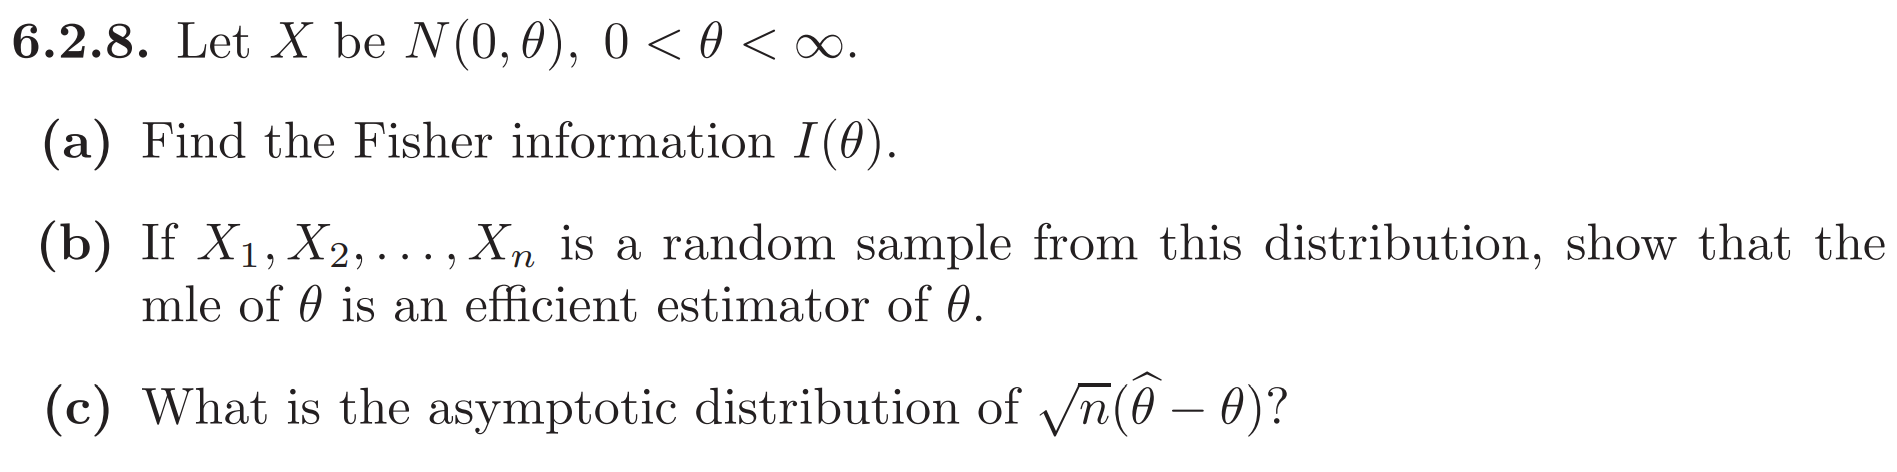
\includegraphics[scale=0.25]{628}
\end{figure}


\noindent \textit{Solution:}

\begin{enumerate}[(a)]
	\item Well, the likelihood is just the pdf:
	\begin{align}
	f(x;\theta) = \f{1}{\sqrt{2\pi \theta}}e^{-x^2/2\theta}, \theta \in \mathbb{R}^+\setminus\{\infty\}.
	\end{align}
	Then, the log likelihood is
	\begin{align}
	l(\theta) = -\f{1}{2}\ln (2\pi \theta) - \f{x^2}{2\theta} \implies \p_\theta l(\theta)  = -\f{1}{2\theta} + \f{x^2}{2\theta^2}.
	\end{align}
	The Fisher information is then 
	\begin{align}
	I(\theta) &= -E[\p^2_\theta l(\theta)]\nn\\
	&= -E\lb \f{1}{2\theta^2} - \f{X^2}{\theta^3}   \rb\nn\\
	&= -\f{1}{2\theta^2} + \f{1}{\theta^3} E[X^2]\nn\\
	&= -\f{1}{2\theta^2} + \f{1}{\theta^3} (\Var[X] + \cancel{E[X]^2})\nn\\
	&= -\f{1}{2\theta^2} + \f{1}{\theta^3} \theta\nn\\
	&= \boxed{\f{1}{2\theta^2}}
	\end{align}
	
	\item We know that the mle of $\theta$ is given by
	\begin{align}
	\hat\theta = \f{1}{n}\sum^n_{i=1}(x_i - 0)^2,
	\end{align}
	which is just the sample variance with denominator $n$. Now, $\hat\theta$ is an unbiased estimator of $\theta$ because
	\begin{align}
	E[\hat\theta] &= \f{1}{n}\sum^n_{i=1}E[X_i^2 + 2X_i\cdot 0 + 0] = \f{1}{n}\sum^n_{i=1}E[X_i^2]= \f{n}{n}\Var[X] = \theta.
	\end{align} 
	Next we want to find $\Var[\hat\theta]$. Well,
	\begin{align}
	\Var[\hat\theta] &= \Var\lb \f{1}{n}\sum^n_{i=1} X_i^2 \rb\nn\\
	&= \f{1}{n^2}\sum^n_{i=1} \Var[X_i^2] \nn\\
	&= \f{n}{n^2}\lp E[X_i^4] - E[X_i^2]^2 \rp\nn\\
	&= \f{n}{n^2}\lp E[X_i^4] - \Var[X_i]^2 \rp\nn\\
	&= \f{n}{n^2}\lp E[X_i^4] - \theta^2 \rp.
	\end{align}
	To find $E[X_i^4]$ we can either brute force:
	\begin{align}
	E[X^4] = \int_\mathbb{R}x^4 \f{1}{\sqrt{2\pi \theta}}e^{-x^2/2\theta}\,dx = 3\theta^2.
	\end{align}
	Or use the MGF:
	\begin{align}
	&M(t) = e^{\cancel{\mu t} + \theta t^2/2}\nn\\
	& \implies E[X^4] = M^{(4)}(0) = (3\theta^2 + 6 t^2 \theta^3 + t^4\theta^4)e^{\theta t^2/2}\bigg\vert_{t=0} = 3\theta^2.
	\end{align}
	And so,
	\begin{align}
	\Var[\hat\theta] = \f{1}{n}\lp 3\theta^2 - \theta^2 \rp = \boxed{\f{2\theta^2}{n}}
	\end{align}
	Because $\Var[\hat\theta] = 2\theta^2/n = 1/nI(\theta)$, the CRLB is attained. Further, because $\hat\theta$ is an unbiased estimator of $\theta$, $\hat\theta$ is an efficient estimator of $\theta$. 
	
	
	
	\item Since all regularity conditions are met, we can use Theorem 6.2.2., which says that 
	\begin{align}
	\sqrt{n}(\hat\theta - \theta) \xrightarrow{D} \N(0, 1/I(\theta)) = \boxed{\N \lp 0,2\theta^2\rp}
	\end{align}
\end{enumerate}\qed













\newpage
\noindent \textbf{6.2.9}
\begin{figure}[!htb]
	\centering
	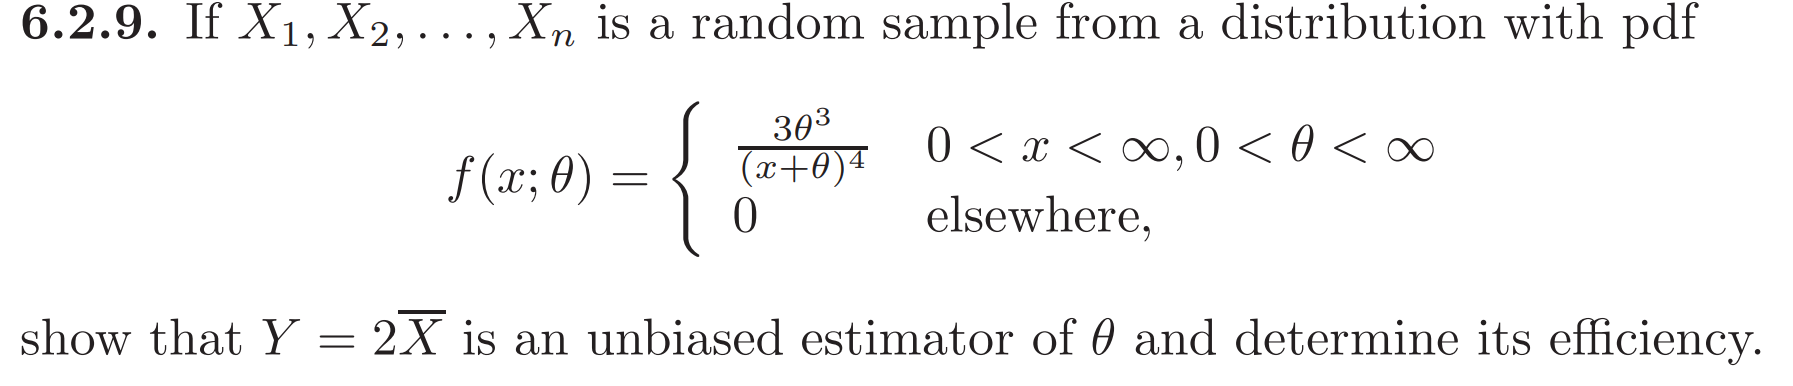
\includegraphics[scale=0.25]{629}
\end{figure}


\noindent \textit{Solution:} Well, we first show that $Y$ is an unbiased estimator of $\theta$:
\begin{align}
E[Y] = 2E[\bar{X}] = \f{2}{n}nE[X_i] = 2E[X_i] = 2\int_0^\infty \f{3x\theta^3}{(x+\theta)^4}\,dx = 2\f{\theta}{2} = \theta.
\end{align}
So, yes, $Y$ is an unbiased estimator of $\theta$. \\

The efficiency of $Y$ is given by
\begin{align}
\epsilon = \f{CRLB}{\Var[Y]} = \f{1}{\Var[Y] \cdot nI(\theta)}
\end{align}
To find this we next find the Fisher information:
\begin{align}
I(\theta) &= -E\lb \p_\theta^2 l(\theta) \rb\nn\\
&=-E\lb \p_\theta^2 \ln \f{3\theta^3}{(X+\theta)^4} \rb\nn\\
&= -E\lb \p_\theta^2 \ln \f{3\theta^3}{(X+\theta)^4} \rb\nn\\
&= -E\lb \f{\theta^2 - 6\theta X - 3X^2}{\theta^2(\theta+X)^2}  \rb\nn\\
&= -\int^\infty_0 \f{\theta^2 - 6\theta x - 3x^2}{\theta^2(\theta+x)^2}\cdot \f{3\theta^3}{(x+\theta)^4} = \f{3}{5\theta^2}.
\end{align}
Next, we find the variance of $Y$:
\begin{align}
\Var[Y] &= \Var[2\bar{X}] = \f{4}{n^2}\Var\lb \sum^n_{i=1} X_i \rb = \f{4n}{n^2}\Var[X_i]= \f{4}{n}\lp E[X_i^2] - E[X_i]^2 \rp\nn\\
&= \f{4}{n} \lc \int_0^\infty \f{3x^2\theta^3}{(x+\theta)^4}\,dx - \lb \int^\infty_0 \f{3x\theta^2}{(x+\theta)^4}\,dx \rb^2\rc\nn\\
&= \f{4}{n}\lp \theta^2 - \f{\theta^2}{4} \rp = \f{3\theta^2}{n}.
\end{align}
So, 
\begin{align}
\epsilon = \f{5\theta^2}{3\theta^2 \cdot 3} = \boxed{\f{5}{9}}
\end{align}










\newpage










\section{Problem set 6}





\noindent \textbf{6.3.1}
\begin{figure}[!htb]
	\centering
	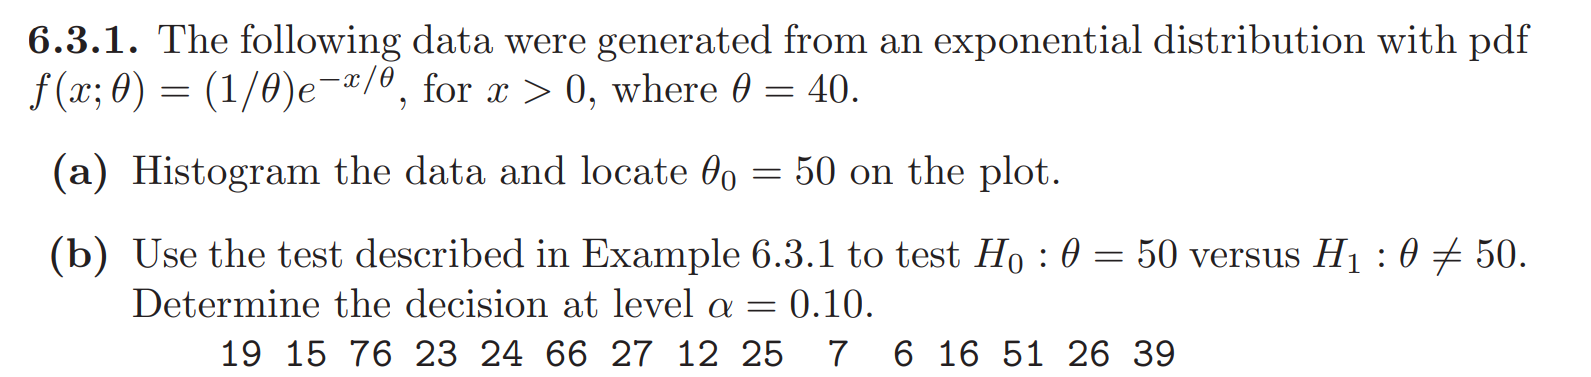
\includegraphics[scale=0.6]{631}
\end{figure}

\noindent \textit{Solution:} 

\begin{enumerate}[(a)]
	\item 
	\textbf{R code:}
	\begin{lstlisting}
	> dt = c(19, 15, 76, 23, 24, 66, 27, 12, 25, 7, 6, 16, 51, 26, 39)
	> hist(dt)
	> abline(v=50)
	\end{lstlisting}
	\begin{figure}[!htb]
		\centering
		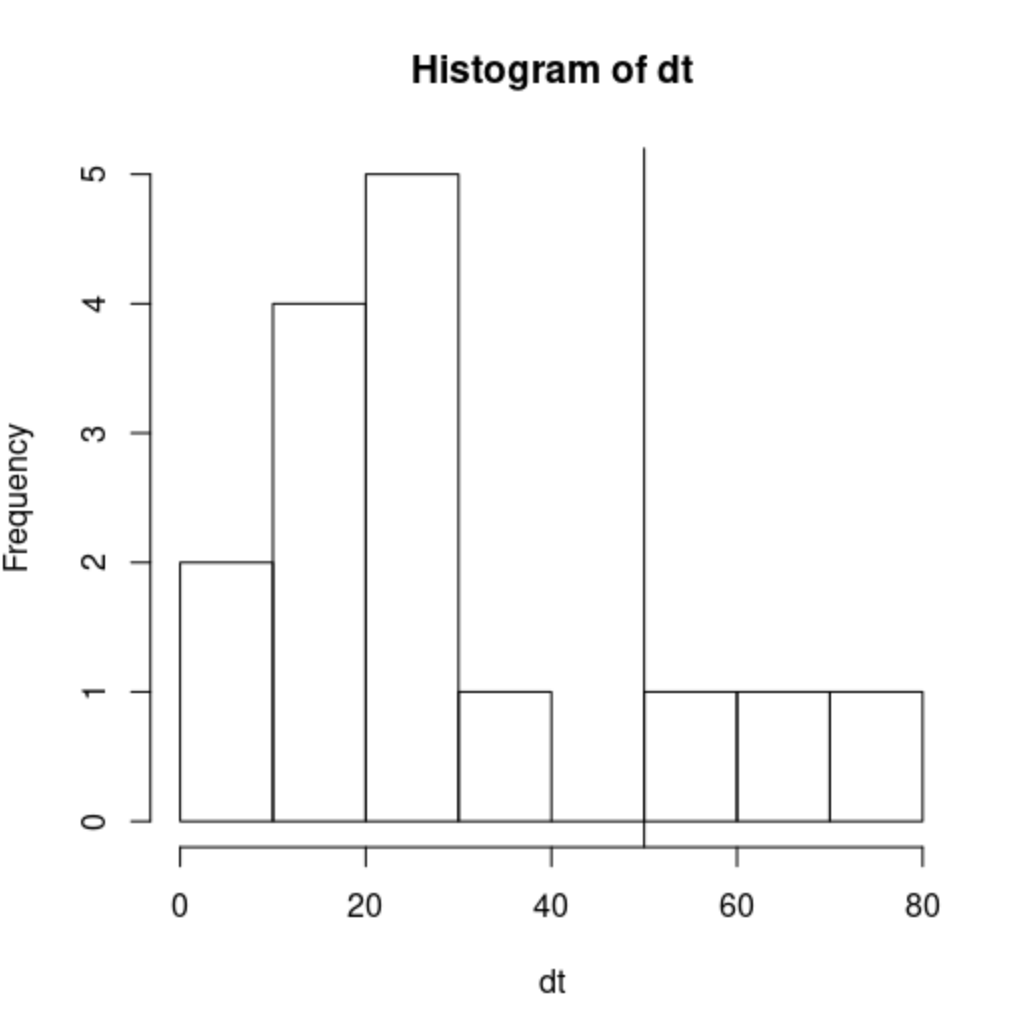
\includegraphics[scale=0.5]{631-hist}
	\end{figure}




	\item $H_0: \theta = 50$, $H_a : \theta \neq 50$. Example 6.3.1 says that we reject $H_0$ if
	\begin{align}
	\f{2}{\theta_0} \sum^n_{i=1}X_i \geq \chi^2_{1-\al/2}(2n)\mbox{ or } \f{2}{\theta_0} \sum^n_{i=1}X_i \leq \chi^2_{\al/2}(2n)
	\end{align}
	In our case, 
	\begin{align}
	\tau = \f{2}{\theta_0} \sum^n_{i=1}X_i  = 17.28,
	\end{align}
	while 
	\begin{align}
	&\chi^2_{0.10/2}(30) = 18.49266\nn\\
	&\chi^2_{1-0.10/2}(30) = 43.77297.
	\end{align}
	Since $\tau < \chi^2_{0.10/2}(30)$, we \textbf{reject} $H_0$.\\
	
	\textbf{R code:}
	\begin{lstlisting}
	> sum(dt)
	[1] 432
	> (2/50)*sum(dt)
	[1] 17.28
	> length(dt)
	[1] 15
	> qchisq(0.10/2,30)
	[1] 18.49266
	> qchisq(1-0.10/2,30)
	[1] 43.77297
	\end{lstlisting}
	\qed
	
	
	
	
	
	
\end{enumerate}


\newpage



\noindent \textbf{6.3.6}
\begin{figure}[!htb]
	\centering
	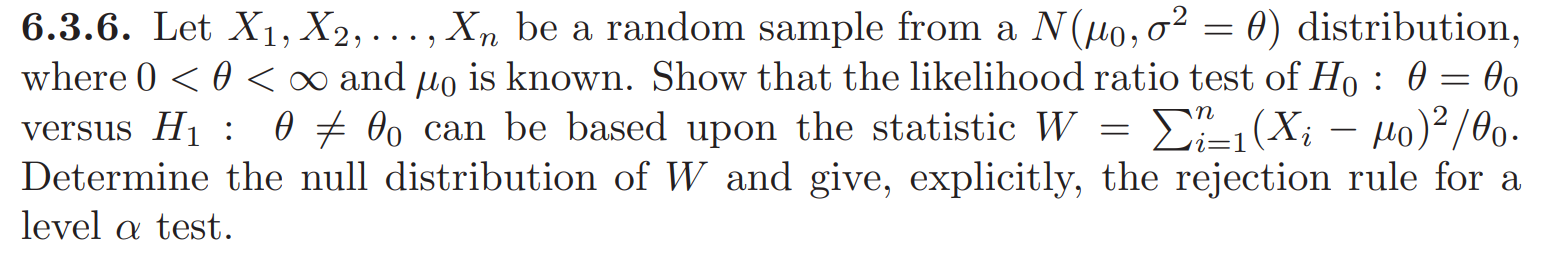
\includegraphics[scale=0.6]{636}
\end{figure}


\noindent \textit{Solution:} 
The mle for $\sigma^2$ is 
\begin{align}
\hat\sigma^2 = \f{1}{n}\sum (X_i  -\mu_0)^2.
\end{align}
With this, 
\begin{align}
\Lambda = \f{\lag(\theta_0)}{\lag(\hat\theta)} = \lp \f{\hat\sigma^2}{\theta_0}\rp^{n/2} \exp\lb \f{-1}{2\theta_0}\sum^n_{i=1}(x_i - \mu_0)^2 + \f{n}{2}\f{\sum(x_i - \mu_0)^2}{\sum(x_i - \mu_0)^2} \rb.
\end{align}
This has the form $\Lambda = n^{-n/2} W^{n/2} e^{-W/2} e^{n/2}$, which is unimodal. So, $\Lambda \leq C \implies W \in (c_1, c_2)$ for some $c_1, c_2$. This says we can use $W$ as a testing statistic. Now, under $H_0: \theta = \theta_0$, we have that $X_i \sim \N(\mu_0, \theta=\theta_0)$, and so $(X_i - \mu_0)/\sqrt{\theta_0} \sim \N(0,1) $. This means $W = \sum^n (X_i - \mu_0)^2/\theta_0 \sim \chi^2(n)$. \\

We reject whenever $W \geq \chi^2_{1-\al/2}(n)$ or $W \leq \chi^2_{\al/2}(n)$. \qed











\newpage
\noindent \textbf{6.3.11}
\begin{figure}[!htb]
	\centering
	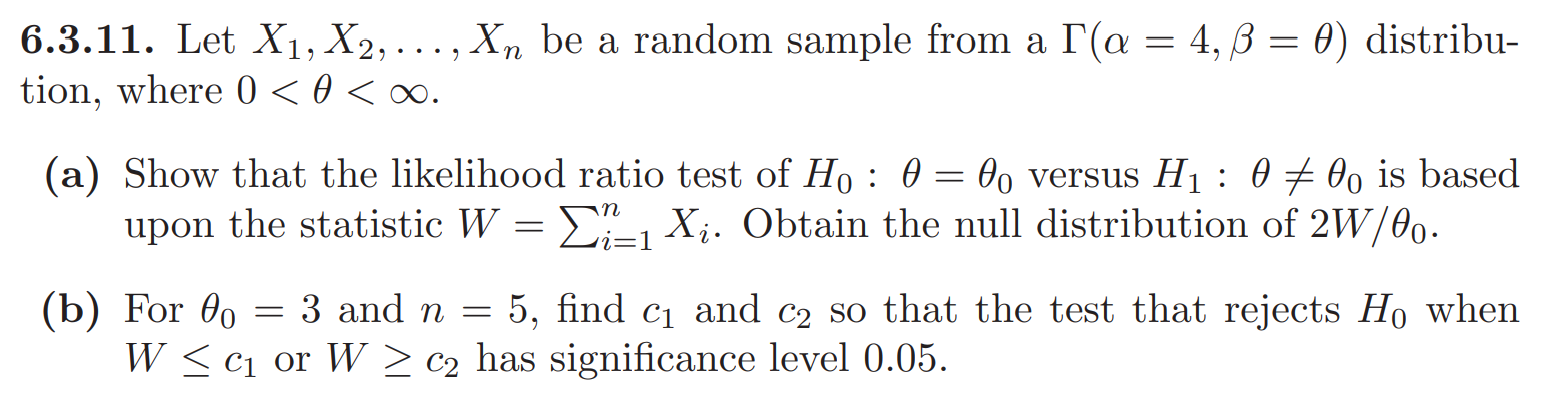
\includegraphics[scale=0.6]{6311}
\end{figure}


\noindent \textit{Solution:} 
\begin{enumerate}[(a)]
	\item 
	We know that
	\begin{align}
	\hat\beta = \f{1}{n\al} \sum^n_{i=1}X_i = \f{\bar{X}}{\al} = \f{\bar{X}}{4}.
	\end{align}
	\begin{align}
	\Lambda &= \f{\lag(\hat\theta)}{\lag (\theta_0)} = \f{1/\hat\theta^{4n}}{1/\theta_0^{4n}} \exp \lb -\lp  \f{1}{\hat\theta}- \f{1}{\theta_0} \rp\sum x_i  \rb\nn\\
	&\sim (4 n)^{-4n}\lp\sum x_i/\theta_0\rp^{-4n} \exp \lb -\sum X_i/\theta_0 \rb \exp\lb 4n \rb\nn\\
	&= (4 n)^{-4n}W^{-4n}\theta_0^{4n} \exp \lb -W/\theta_0 \rb \exp\lb 4n \rb.
	\end{align}
	So, $\Lambda$ depends on $W$ as desired. Now, since $X_i \sim \Gamma(4,\theta_0)$ under $H_0$, we have
	\begin{align}
	\f{2W}{\theta_0} = \f{2}{\theta_0}\sum X_i \sim \Gamma\lp n\al, \f{2\theta_0}{\theta_0} \rp = \Gamma(4n,2) = \boxed{\chi^2(4n)}
	\end{align} 
	
	
	\item 
	\begin{align}
	c_1 = \f{\theta_0}{2}\chi^2_{\al/2}(4n) = \f{3}{2}\times 9.590777 = \boxed{14.38617}\nn\\
	c_2 = \f{\theta_0}{2}\chi^2_{1-\al/2}(4n) = \f{3}{2}\times 34.16961 = \boxed{51.25441}
	\end{align}
	
	
	\textbf{R code:}
	\begin{lstlisting}
	> qchisq(1-0.05/2,4*5)
	[1] 34.16961
	> qchisq(0.05/2,4*5)
	[1] 9.590777
	> 34.16961*1.5
	[1] 51.25441
	> 9.590777*1.5
	[1] 14.38617 
	\end{lstlisting}
\end{enumerate}\qed










\newpage
\noindent \textbf{6.3.18}
\begin{figure}[!htb]
	\centering
	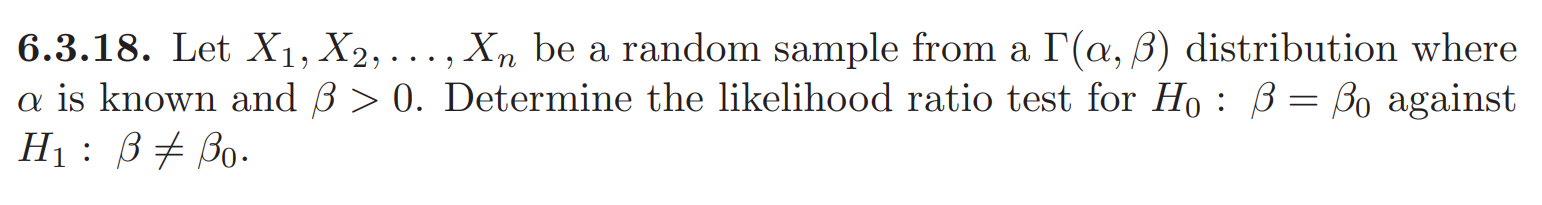
\includegraphics[scale=0.6]{6318}
\end{figure}


\noindent \textit{Solution:} The setup of this problem is exactly like that of 6.3.11. The likelihood ratio test of $H_0 : \beta = \beta_0$ versus $H_a : \beta \neq \beta_0$ is based upon the statistic $W = \sum X_i $. The null distribution of $2W/\beta_0$ is $\chi^2(n\al)$, under $H_0$. We reject whenever $W \leq c_1$ or $W \geq c_2$, where 
\begin{align}
&c_1 = \f{\beta_0}{2}\chi^2_{\al/2}(\al n) \nn\\
&c_2 = \f{\beta_0}{2}\chi^2_{1-\al/2}(\al n). 
\end{align}

\qed


\newpage
\noindent \textbf{6.4.1}
\begin{figure}[!htb]
	\centering
	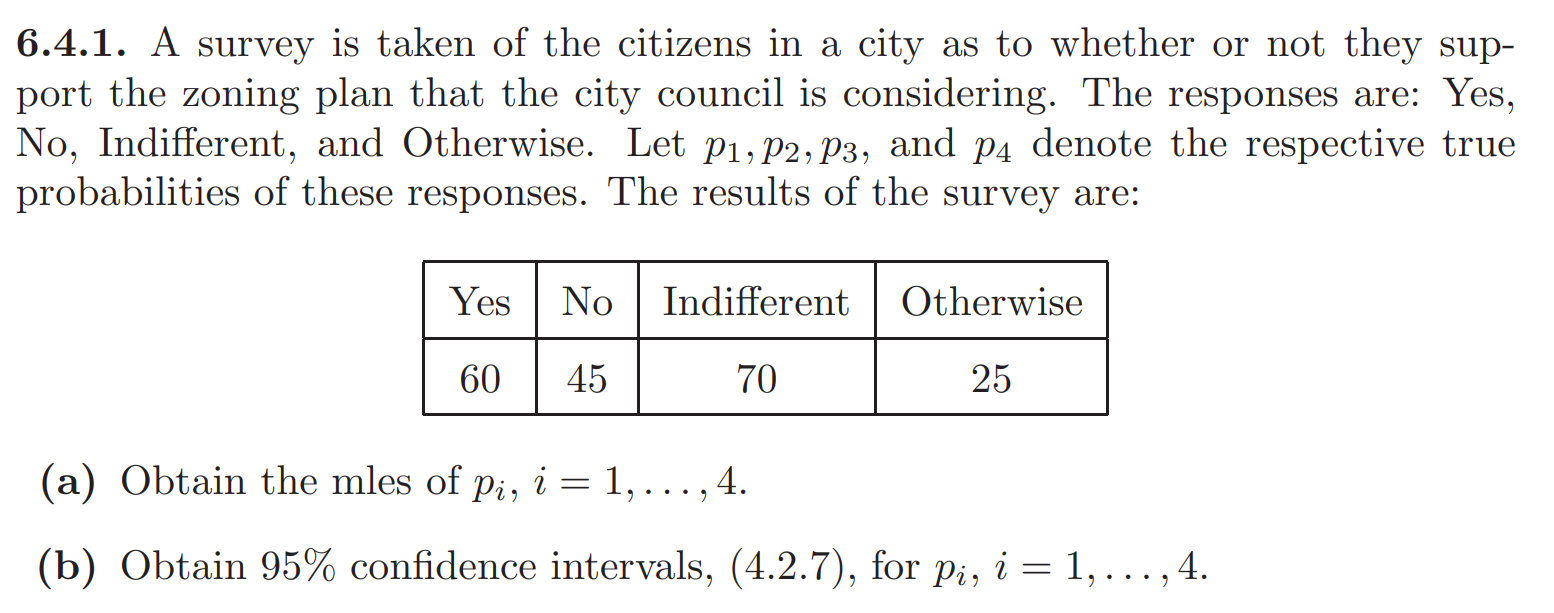
\includegraphics[scale=0.6]{641}
\end{figure}


\noindent \textit{Solution:} 
\begin{enumerate}[(a)]
	\item The mle for each $p_i$ is 
	\begin{align}
	\hat{p}_i = \f{\mbox{\# Observations of $i$}}{n}.
	\end{align}
	
	\item 
	\begin{align}
	CI_1 &= \lp \hat{p}_1 - z_{\al/2}\sqrt{\hat{p}_1(1-\hat{p}_1)/n}, \hat{p}_1 + z_{\al/2}\sqrt{\hat{p}_1(1-\hat{p}_1)/n} \rp \nn\\
	&= \lp \f{60}{200} - 1.96\times 0.0324037 , \f{60}{200} + 1.96\times 0.0324037  \rp\nn\\ 
	&= \boxed{(0.2364887, 0.3635113)}
	\end{align}
	\begin{align}
	CI_2 
	&= \lp \f{45}{200} - 1.96\times 0.02952753 , \f{45}{200} + 1.96\times 0.02952753  \rp\nn\\ 
	&= \boxed{(0.167126, 0.282874)}
	\end{align}
	\begin{align}
	CI_3
	&= \lp \f{70}{200} - 1.96\times 0.03372684 , \f{70}{200} + 1.96\times 0.03372684  \rp\nn\\ 
	&= \boxed{(0.2838954, 0.4161046)}
	\end{align}
	\begin{align}
	CI_4 
	&= \lp \f{25}{200} - 1.96\times 0.02338536  , \f{25}{200} + 1.96\times 0.02338536  \rp\nn\\ 
	&= \boxed{(0.0791647, 0.7732091)}
	\end{align}
	
\end{enumerate}\qed





\newpage
\noindent \textbf{6.4.3}
\begin{figure}[!htb]
	\centering
	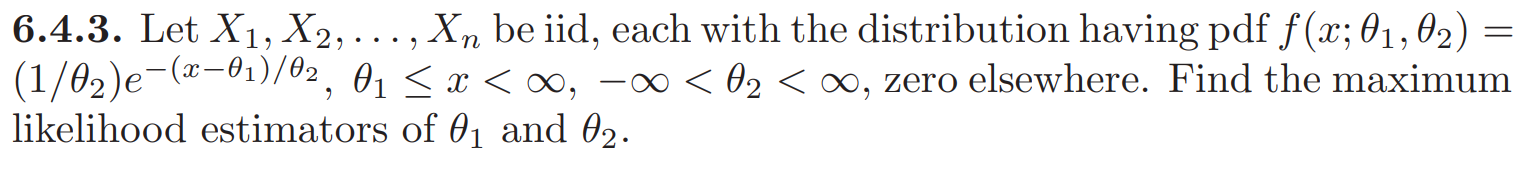
\includegraphics[scale=0.6]{643}
\end{figure}

\noindent \textit{Solution:}  The likelihood function is 
\begin{align}
\lag(\theta_1, \theta_2) = \f{1}{\theta_2^n} \exp \lb -\f{1}{\theta_2}\sum^n_{i=1} (x_i - \theta_1) \rb.
\end{align}
with the support given in the problem. We find 
\begin{align}
\ln \lag = -n \ln \theta_2 - \f{1}{\theta_2}\sum^n_{i=1}(x_i - \theta_1).
\end{align}
And so,
\begin{align}
\p_{\theta_1} \ln \lag(\theta_1,\theta_2) = \f{n}{\theta_2} > 0  \implies \boxed{\hat\theta_1 = \text{Argmax}\ln\lag(\theta_1,\theta_2) = \min_i X_i }\nn\\
\p_{\theta_2} \ln \lag(\hat\theta_1,\theta_2) = -\f{n}{\theta_2} + \f{1}{\theta_2^2} \sum^n_{i=1}\lp x_i - \hat\theta_1 \rp = 0 \implies \boxed{\hat\theta_2 = \f{1}{n}\sum^n_{i=1}(X_i - \min_i X_i) }
\end{align}
where we have used $\hat\theta_1 = \min_i X_i$ in writing the mle for $\theta_2$. \qed


\newpage
\noindent \textbf{6.4.5}
\begin{figure}[!htb]
	\centering
	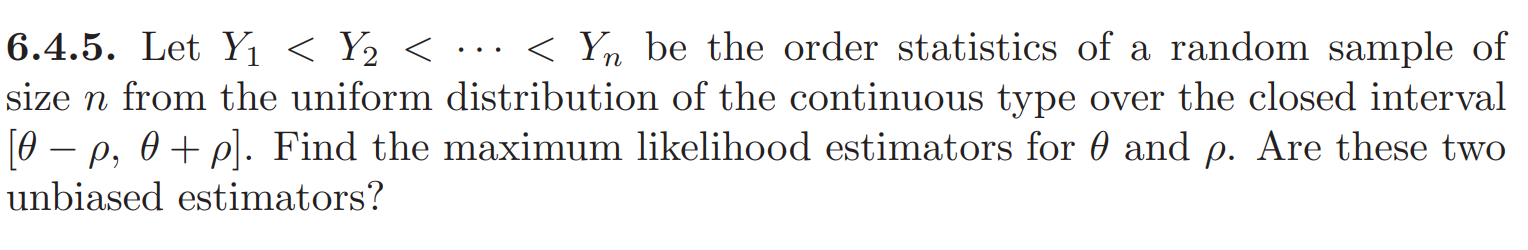
\includegraphics[scale=0.6]{645}
\end{figure}


\noindent \textit{Solution:} It's not difficult to see that
\begin{align}
&\hat\theta - \hat\rho = \min Y_i = Y_1\nn\\
&\hat\theta + \hat\rho = \max Y_i = Y_n.
\end{align}
Solving this for $\hat\theta, \hat\rho$ gives
\begin{align}
&\hat\theta = \f{Y_n + Y_1}{2}\nn\\
&\hat\rho = \f{Y_n - Y_1}{2}.
\end{align}
Next, 
\begin{align}
F_{Y_1}(x) = P(Y_1 \leq x) &= P(\min_i Y_i \leq x)\nn\\
&= 1 - P(\min_i Y_i > x)\nn\\
&= 1 - \prod^n_{i=1}P(Y_i > x)\nn\\
&= 1 - (1 - F_{Y_i}(x))^n = 1 - \lp 1- \int^x_{\theta-\rho}\f{1}{2\rho}\,dx \rp^n\nn\\
&= 1 - \lp 1- \f{x-\theta+\rho}{2\rho} \rp^n\nn\\
\implies  f_{Y_1}(x) &= \f{n(\theta + \rho - x)^{n-1}}{(2\rho)^n}
\end{align}
And so, 
\begin{align}
E[Y_1] = \int_{\theta-\rho}^{\theta+\rho} x\f{n(\theta + \rho - x)^{n-1}}{(2\rho)^n}\,dx = \f{1 - n }{1 + n} \rho + \theta
\end{align}
Next, 
\begin{align}
F_{Y_n}(x) = P(Y_n \leq x) &= P(\max_i Y_i \leq x)\nn\\
&= \prod^n_{i=1}P(Y_i \leq x) = \prod^n_{i=1}F_{Y_i}\nn\\
&= \f{(x-\theta+\rho)^{n}}{(2\rho)^n}\nn\\
\implies f_{Y_n}(x) &= \f{n(x-\theta+\rho)^{n-1}}{(2\rho)^n}.
\end{align}
And so,
\begin{align}
E[Y_n] = \int^{\theta+\rho}_{\theta-\rho} x \f{n(x-\theta+\rho)^{n-1}}{(2\rho)^n}\,dx = \f{n-1}{n+1}\rho + \theta.
\end{align}
With these,
\begin{align}
E[\hat\theta] = E\lb \f{Y_n + Y_1}{2} \rb = \f{1}{2}E\lb 2\theta\rb &= \theta\nn\\
E[\hat\rho] = E\lb \f{Y_n - Y_1}{2} \rb = \f{1}{2}E\lb \f{n-1-1+n}{n+1}\rho \rb &= \rho.
\end{align}
So, $\hat\theta$ and $\hat\rho$ are unbiased. \qed

















\newpage
\noindent \textbf{6.5.3}
\begin{figure}[!htb]
	\centering
	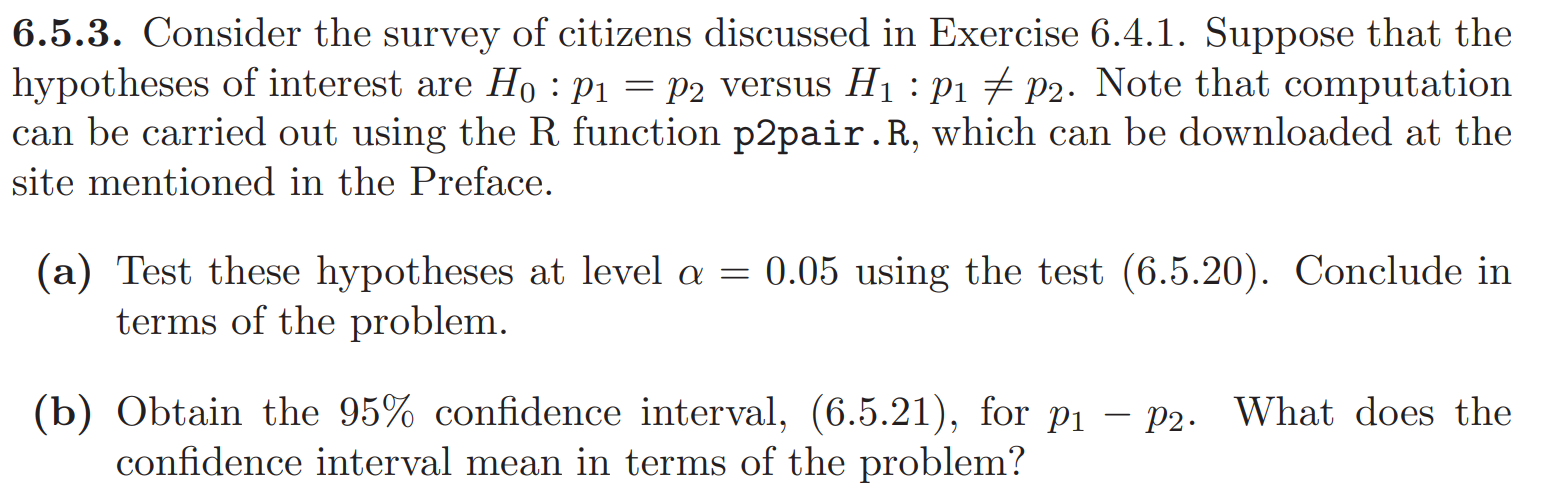
\includegraphics[scale=0.6]{653}
\end{figure}


\noindent \textit{Solution:} 
\begin{enumerate}[(a)]
	\item $H_0 : p_1 = p_2$ and $H_a : p_1 \neq p_2$. 
	\begin{align}
	\chi^2_W &= \f{(\hat{p}_1 - \hat{p}_2)^2}{(\hat{p}_1 + \hat{p}_2 - (\hat{p}_1 - \hat{p}_2)^2 )/n} \nn\\
	&= \f{(60/200 - 45/200)^2}{(60/200 + 45/200 - (60/200 - 45/200)^2 )/200}\nn\\
	&= \boxed{2.167}
	\end{align}
	Clearly, $2.167 < 3.81 = \chi^2_{0.05}(1)$. So, we fail to reject $H_0$ -- there is not enough evidence to reject the null hypothesis that the proportions of people who vote Yes and No are the same.
	
	
	
	\item The 95\% CI for $p_1 - p_2$ is 
	\begin{align}
	&\lp \f{60}{200} - \f{45}{200} \rp \pm z_{0.05/2}\lp \f{\f{60}{200} + \f{45}{200} - \lp \f{60}{200} - \f{45}{200} \rp^2}{200} \rp^{1/2}\\
	&= \lp   -0.025  ,  0.175  \rp.
	\end{align}
	Since the CI contains 0, we fail to reject $H_0$. 
	
	
\end{enumerate}\qed












\newpage
\noindent \textbf{6.5.6}
\begin{figure}[!htb]
	\centering
	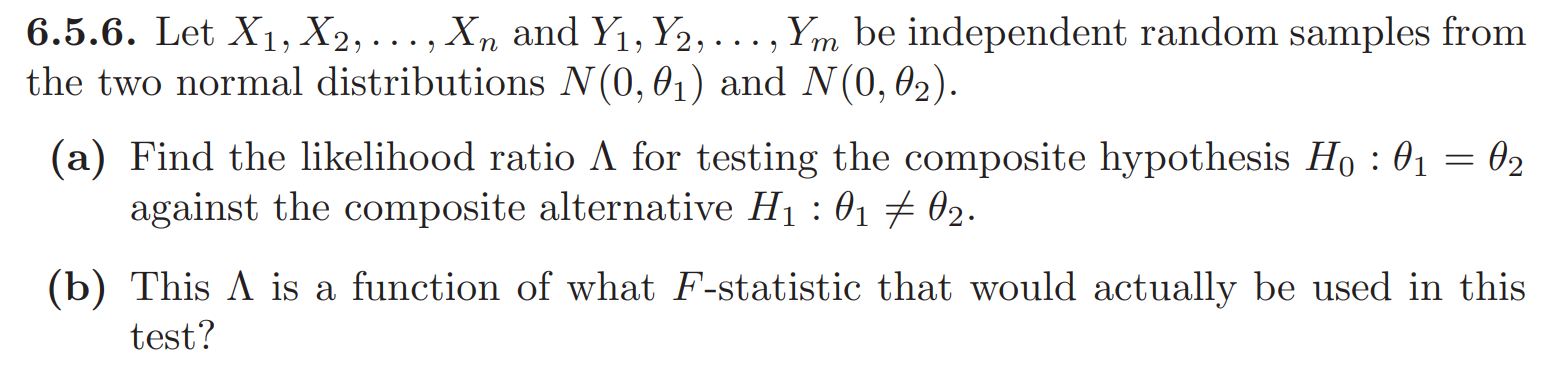
\includegraphics[scale=0.6]{656}
\end{figure}


\noindent \textit{Solution:} 
\begin{enumerate}[(a)]
	\item $H_0 : \theta_1 = \theta_2$ and $H_a : \theta_1 \neq \theta_2$. $X_i \sim \N(0,\theta_1)$ and $Y_i \sim \N(0, \theta_2)$. So,
	\begin{align}
	\lag(\theta_1,\theta_2) = (2\pi \theta_1)^{-n/2}(2\pi \theta_2)^{-m/2} \exp \lb -\f{1}{2\theta_1}\sum^n_{i=1} x_i^2  - \f{1}{2\theta_2}\sum^m_{i=1} y_i^2 \rb.
	\end{align}
	Under $H_0: \theta_1 = \theta_2$:
	\begin{align}
	\p_\theta \ln \lag(\theta_1 = \theta_2 = \theta) = 0 &\implies -\f{n+m}{2} -\f{1}{2\theta}\lb \sum^n x_i^2 + \sum^m y_i^2 \rb  = 0 \nn\\
	&\implies \hat\theta = \f{1}{n+m} \lb  \sum^n x_i^2 + \sum^m y_i^2 \rb.
	\end{align}
	With this, 
	\begin{align}
	\lag(\hat\Theta_0) &= \lp \f{2\pi}{n+m}\lb \sum^n x_i^2 + \sum^m y_i^2 \rb \rp^{-\f{n+m}{2}} \exp\lb -\f{\sum^n x_i^2 + \sum^m y_i^2}{\f{2}{n+m}\lp \sum^n x_i^2 + \sum^m y_i^2 \rp}  \rb\nn\\
	&= \lp \f{2\pi}{n+m}\lb \sum^n x_i^2 + \sum^m y_i^2 \rb \rp^{-\f{n+m}{2}} \exp\lb \f{-n-m}{2}\rb.
	\end{align}
	In the joint space, 
	\begin{align}
	&\hat\theta_1 = \f{1}{n}\sum^n x_i^2\nn\\
	&\hat\theta_2 = \f{1}{m}\sum^m y_i^2.
	\end{align}
	With these,
	\begin{align}
	\lag(\hat\Theta) = \lp \f{2\pi}{n}\sum^n x_i^2 \rp^{-n/2} \lp \f{2\pi}{m}\sum^m y_i^2 \rp^{-m/2} \exp\lb \f{-n-m}{2} \rb.
	\end{align}
	And so we have
	\begin{align}
	\Lambda &= \f{\lag_0}{\lag} = \f{\lp \f{1}{n+m}\lb \sum^n x_i^2 + \sum^m y_i^2 \rb \rp^{-\f{n+m}{2}}}{\lp \f{1}{n}\sum^n x_i^2 \rp^{-n/2} \lp \f{1}{m}\sum^m y_i^2 \rp^{-m/2}}\nn\\
	&= \f{(n+m)^{\f{n+m}{2}}}{n^{n/2} m^{m/2}} \f{\lp \sum^n x_i^2 \rp^{n/2} \lp \sum^m y_i^2 \rp^{m/2}}{\lb \sum^n x_i^2 + \sum^m y_i^2 \rb ^{\f{n+m}{2}}}\nn\\
	&= \f{(n+m)^{\f{n+m}{2}}}{n^{n/2} m^{m/2}} \lp \underbrace{\f{\sum^n x_i^2}{\sum^n x_i^2 + \sum^m y_i^2 }}_{T} \rp^{n/2} \lp\underbrace{ \f{\sum^n x_i^2}{\sum^m y_i^2 + \sum^m y_i^2 }}_{1-T}  \rp^{m/2}.
	\end{align}
	
	
	\item $\Lambda \leq k$ is equivalent to $W \leq c_1$ or $W \geq c_2$ with 
	\begin{align}
	\boxed{W = \f{\f{1}{n}\sum^n x_i^2 }{\f{1}{m}\sum^m y_i^2} \sim F(n,m)}
	\end{align}
	such that $1/T = 1 + 1/W$. This is because $\sum^n x_i^2/\theta \sim \chi^2(n), \sum^m y_i^2/\theta \sim \chi^2(m)$ under $H_0$.
\end{enumerate}\qed









\newpage
\noindent \textbf{6.5.7}
\begin{figure}[!htb]
	\centering
	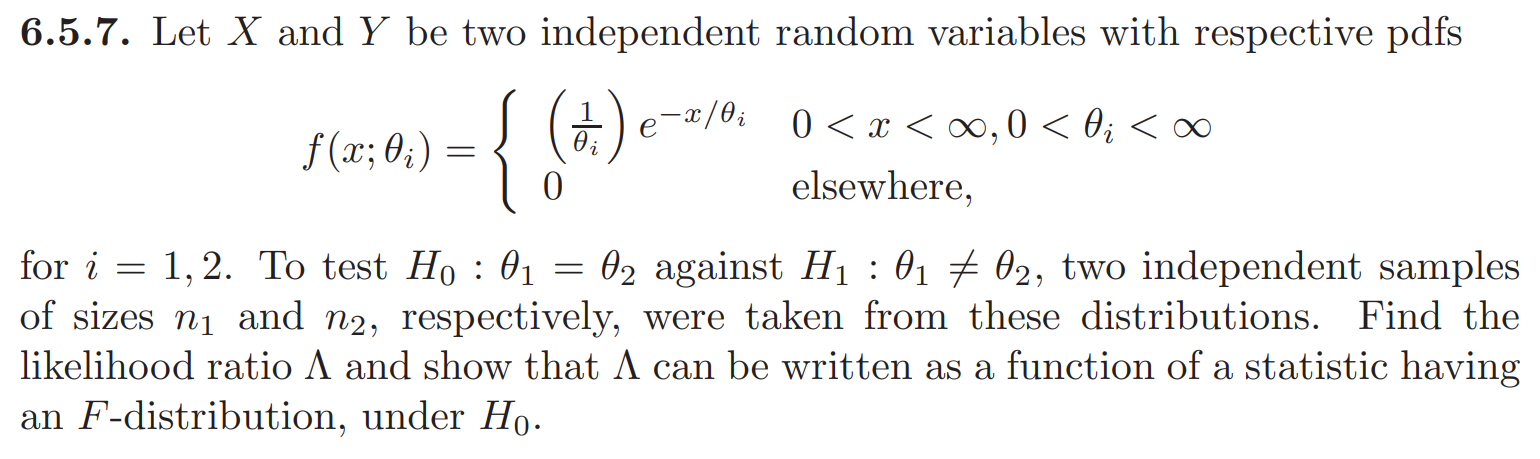
\includegraphics[scale=0.6]{657}
\end{figure}


\noindent \textit{Solution:} We did this in ``class,'' so I will skip a few steps. Let $X_i \sim \exp (\theta_1)$ and $Y_i \sim \exp(\theta_2)$. $H_0 : \theta_1 = \theta_2$ and $H_a : \theta_1 \neq \theta_2$. The null space is $\{ \{ \theta_1,\theta_2\}: \theta_1 = \theta_2 > 0 \}$. The alternative space is $\{ \{ \theta_1,\theta_2 \}: \theta_1 \neq \theta_2, \theta_1,\theta_2 \neq 0 \}$. The joint space is just $\{ \{ \theta_1,\theta_2 \}, \theta_1 >0, \theta_2 > 0 \}$. It's easy to see that
\begin{align}
\lag(\theta_1,\theta_2 \vert X,Y) = \f{1}{\theta_1^n}e^{\sum^n x_i/\theta_1} \f{1}{\theta_2^m}e^{\sum^m y_i/\theta_2} .
\end{align}
From here one finds that under $H_0: \theta_1 = \theta_2 = \theta$:
\begin{align}
l(\Theta_0) = -(n+m) \ln\theta-\f{1}{\theta}\lp \sum x_i + \sum y_i \rp.
\end{align}
And so
\begin{align}
\p_\theta l(\theta) = 0 \implies \hat\theta_0 = \f{1}{n+m} \lp \sum x_i + \sum y_i \rp.
\end{align}
With this, we can plug back in to calculate the numerator:
\begin{align}
\lag(\hat\Theta_0) = \dots = \lp\f{1}{n+m} \lb\sum x_i + \sum y_j \rb \rp^{-n-m} \exp(-n-m).
\end{align}
In the joint space, 
\begin{align}
l(\Theta) = -n \ln \theta - \f{1}{\theta}\sum x_i - m \ln \mu - \f{1}{\mu}\sum y_j.
\end{align}
And so
\begin{align}
\p_{\theta_1} l(\Theta) = 0 \implies \hat\theta_1 = \bar{x}\\
\p_{\theta_2} l(\Theta) = 0 \implies \hat\theta_2 =  \bar{y}.
\end{align}
With these,
\begin{align}
\lag(\hat\Theta) &= \dots\\
&= \f{1}{\lp \f{1}{n}\sum x_i \rp^n} \exp \lb -\f{1}{\f{1}{n}\sum x_i} \sum x_i\rb  
\f{1}{\lp \f{1}{m}\sum y_i \rp^m} \exp \lb -\f{1}{\f{1}{m}\sum y_i} \sum y_i\rb\\
&=\f{1}{\lp \f{1}{n}\sum x_i \rp^n} e^{-n} \f{1}{\lp \f{1}{m}\sum y_i \rp^m} e^{-m}.
\end{align}
Putting everything together, we find
\begin{align}
\Lambda = \f{\lag_0}{\lag} = \dots = \f{\f{1}{(n+m)^{-n-m}} \lp \sum x_i + \sum y_j \rp^{-n-m}   }{\f{1}{n^n} \f{1}{m^m} \lp \sum x_i \rp^{-n} \lp \sum y_i \rp^{-m}}.
\end{align}
We reject if $\Lambda < c$, iff
\begin{align}
\f{(n+m)^{n+m}}{n^n m^m} \f{\lp \sum x_i \rp^{n} \lp \sum y_i \rp^{m}}{\lp \sum x_i + \sum y_j \rp^{n+m} } < c
\end{align}
iff (letting $c$ absorb the constant)
\begin{align}
\f{\lp \sum x_i \rp^{n} \lp \sum y_i \rp^{m}}{\lp \sum x_i + \sum y_j \rp^{n+m} } < c'
\end{align}


What does the distribution of $\Lambda$ look like? Notice that we reject if
\begin{align}
\Lambda &= \f{(n+m)^{n+m}}{n^n m^m} \f{\lp \sum x_i \rp^{n} \lp \sum y_i \rp^{m}}{\lp \sum x_i + \sum y_j \rp^{n+m} }\\
&= \f{(n+m)^{n+m}}{n^n m^m}\lp \f{ \sum x_i}{ \sum x_i + \sum y_j  }  \rp^n\lp \f{ \sum y_i}{ \sum x_i + \sum y_j  }  \rp^m \\
&= \f{(n+m)^{n+m}}{n^n m^m} T^n (1-T)^{m} < c
\end{align}
which is akin to saying that we reject if $T < a$ or $T > b$. What is the distribution of $T$ under $H_0$? Note that under $H_0$, $\sum x_i \sim \Gamma(n,\theta)$ and $\sum y_i \sim \Gamma(m, \theta)$. By transformation method, we can show that $\boxed{T \sim \beta(n,m)}$. \\


Notice that 
\begin{align}
\f{1}{T} = 1 + \f{\sum y_j}{\sum x_i} =  1 + \f{m}{n}\f{\sum y_j/m}{\sum x_i/n}
\end{align}
Since $\sum X_i \sim  \Gamma(n,\theta), \sum Y_i \sim \Gamma(m,\theta)$ under $H_0$ we have that $2\theta X_i \sim \chi^2(2n)$ and $2\theta Y_i \sim \chi^2(2m)$. This means we can call
\begin{align}
\boxed{W = \f{\sum y_j/m}{\sum x_i/n} = \f{2\theta \sum y_i/m}{2\theta \sum x_i/n} \sim F(2m,2n)}. 
\end{align}

\qed


\newpage






































\section{Problem set 7}

\noindent \textbf{7.2.1}
\begin{figure}[!htb]
	\centering
	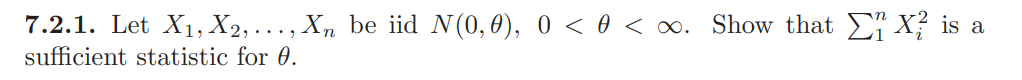
\includegraphics[scale=1]{721}
\end{figure}



\noindent \textit{Solution:} On the one hand
\begin{align}
\prod^n_{i=1} f(x_i;\theta) = (2\pi \theta)^{-n/2}e^{-\sum x_i^2/2\theta}.
\end{align}
On the other hand, $x_i/\sqrt{\theta} \sim \N(0,1)$, which means $Y = \sum X_i^2/\theta \sim \chi^2(n)$, whose pdf is 
\begin{align}
f_{Y}\lp\sum X_i^2/\theta\rp = \f{1}{2^{n/2}\Gamma(n/2)}\lp\sum X_i^2/\theta\rp^{n/2-1}e^{-\lp\sum X_i^2/\theta\rp/2}.
\end{align}
And so,
\begin{align}
\f{(2\pi \theta)^{-n/2}e^{-\sum x_i^2/2\theta}}{\theta^{-1} \f{1}{2^{n/2}\Gamma(n/2)}\lp\sum X_i^2/\theta\rp^{n/2-1}e^{-\lp\sum X_i^2/\theta\rp/2} } \mbox{ is independent of } \theta,
\end{align}
where the factor $\theta^{-1}$ in the denominator comes from the scaling Jacobian. Since the ratio is independent of $\theta$, we say $\sum X_i^2$ is sufficient. \\



Alternative, we can also use the factorization theorem here, with $k_2 = 1$ and $k_1 = \prod f(x_i; \theta)$. \qed 




\newpage




\noindent\textbf{7.2.4}
\begin{figure}[!htb]
	\centering
	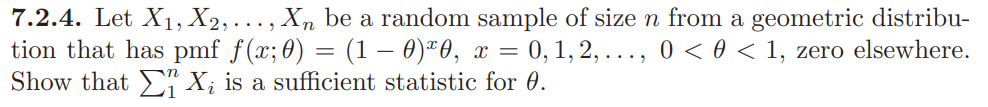
\includegraphics[scale=1]{724}
\end{figure}




\noindent \textit{Solution:} On the one hand,
\begin{align}
A = \prod^n_{i=1}f(x_i;\theta) = (1-\theta)^{\sum x_i}\theta^n.
\end{align}
On the other hand, since each $X_i \sim \mbox{Geom}(\theta)$, the sum $Y = \sum^n_{i=1} X_i \sim \mbox{NegBin}(n,\theta)$, which means 
\begin{align*}
B = f_Y\lp y=\sum x_i \rp = {{\sum x_i+r-1}\choose{\sum x_i}} \theta^n (1-\theta)^{\sum x_i}
\end{align*}
Clearly, the ratio is independent of $\theta$, so we say $\sum X_i$ is sufficient. \\

Alternative, we can also use the factorization theorem, with $k_2 = 1$ and $k_1 = A$. \qed



\newpage


\noindent\textbf{7.2.7}
\begin{figure}[!htb]
	\centering
	\includegraphics[scale=1]{727}
\end{figure}




\noindent \textit{Solution:} Let $X_1,\dots, X_n$ be iid r.v. from $\Gamma(\theta,\be)$. Consider $Y = \prod X_i$. Then we have
\begin{align*}
\prod^n_{i=1} f(x_i;\theta) = \lb \f{1}{\Gamma(\theta)^n \beta^{n\theta}}\prod^n_{i=1}x_i^{\theta-1}\rb \lb  e^{\sum x_i/\beta} \rb
\end{align*} 
where $\beta = 6$ is fixed. We can identify the first term as $k_1$ and the second term as $k_2$. $k_1, k_2$ are both nonnegative functions. $k_1$ is a function of $Y$ and $\theta$, and $k_2$ is a function of only the data. So the factorization theorem tells us $Y$ is sufficient. \qed



\newpage



\noindent\textbf{7.2.8}
\begin{figure}[!htb]
	\centering
	\includegraphics[scale=1]{728}
\end{figure}



\noindent \textit{Solution:} Let $X_1,\dots,X_n$ be iid r.v. from $B(\theta,\theta)$, then 
\begin{align}
f(x_i;\theta) = \f{\Gamma(2\theta)x_i^{\theta-1}(1-x_i)^{\theta-1}}{\Gamma^2(\theta)}
\end{align}
So,
\begin{align}
\prod^n_{i=1}f(x_i;\theta) = \f{\Gamma^n(2\theta)\prod^n_{i=1}\lb x_i^{\theta-1}(1-x_i)^{\theta-1}\rb}{\Gamma^{2n}(\theta)}
\end{align}
We identify
\begin{align*}
\prod^n_{i=1} \lb x_i(1-x_i) \rb^{\theta-1}
\end{align*}
as a sufficient statistic by the factorization theorem, where $k_1$ is the entire $\prod^n_{i=1}f(x_i;\theta)$ and $k_2 = 1$. \qed



\newpage



\noindent\textbf{7.3.1} (Do only for exercises 7.2.1 and 7.2.4)
\begin{figure}[!htb]
	\centering
	\includegraphics[scale=1]{731}
\end{figure}




\noindent \textit{Solution:} Going back to 7.2.1 and 7.2.4 we see that this is the case. In both exercises, we can just set $k_2 = 1$ and $k_1 = \prod^n_{i=1}f(x_i;\theta) = \lag(x_i;\theta)$ and we can easily see that the mle of $\theta$ is a function of the sufficient statistic for $\theta$.  \\

In 7.2.1, the mle of $\theta$ is $(1/n)\sum^n_{i=1}X_i^2$, and the sufficient statistic for $\theta$ is $\sum^n_{i=1}X_i^2$. So, $\hat\theta = (1/n)Y_\theta$ where $Y_\theta$ is the sufficient statistic for $\theta$.\\

For 7.2.4, we have to find the mle of $\theta$. Well, the log likelihood is 
\begin{align*}
\p_\theta l(\theta) = \sum x_i\f{-1}{1-\theta} + \f{n}{\theta} = 0 \implies \hat\theta = \f{1}{\bar{X}+1}.
\end{align*} 
Of course, $\hat\theta$ is a function of the sum of the observations, $\sum X_i$, which is the sufficient statistic for $\theta$. \qed



\qed
\newpage



\noindent\textbf{7.3.3}
\begin{figure}[!htb]
	\centering
	\includegraphics[scale=1]{733}
\end{figure}



\noindent \textit{Solution:}
\newpage





\noindent\textbf{7.3.4}
\begin{figure}[!htb]
	\centering
	\includegraphics[scale=1]{734}
\end{figure}



\noindent \textit{Solution:}
\newpage





\noindent\textbf{7.4.3}
\begin{figure}[!htb]
	\centering
	\includegraphics[scale=1]{743}
\end{figure}



\noindent \textit{Solution:}
\newpage





\noindent\textbf{7.4.5}
\begin{figure}[!htb]
	\centering
	\includegraphics[scale=1]{745}
\end{figure}



\noindent \textit{Solution:}
\newpage





\noindent\textbf{7.4.9}
\begin{figure}[!htb]
	\centering
	\includegraphics[scale=1]{749}
\end{figure}



\noindent \textit{Solution:}
\newpage






\noindent\textbf{7.5.1}
\begin{figure}[!htb]
	\centering
	\includegraphics[scale=1]{751}
\end{figure}



\noindent \textit{Solution:}



\newpage





\noindent\textbf{7.5.3}
\begin{figure}[!htb]
	\centering
	\includegraphics[scale=1]{753}
\end{figure}
\noindent \textit{Solution:}
\newpage






\section{Problem set 8}




\newpage

	
	
\end{document}